Example dynamical system used in this code: \textbf{Lotka-Volterra} system with \textbf{half of the time points} \textbf{unobserved}. The ODE parameters are also unobserved.


\section{User Input}
\subsection{Simulation Settings}
\vspace{1em}
\begin{itemize}
   \item \textbf{true ODE parameter}: Input a row vector of real numbers of size 1 x 4:
    \color{RoyalPurple}\begin{verbatim}
simulation.ode_param = [2,1,4,1];
\end{verbatim}
\color{black}

   \item \textbf{final time for simulation}: Input a positive real number:
    \color{RoyalPurple}\begin{verbatim}
simulation.final_time = 2;
\end{verbatim}
\color{black}

   \item \textbf{observation noise}: Input a function handle:
    \color{RoyalPurple}\begin{verbatim}
simulation.state_obs_variance = @(mean)(bsxfun(@times,[0.5^2,0.5^2],...
ones(size(mean))));
\end{verbatim}
\color{black}

   \item \textbf{time interval between observations}: Input a positive real number:
    \color{RoyalPurple}\begin{verbatim}
simulation.interval_between_observations = 0.1;
\end{verbatim}
\color{black}
\end{itemize}

\vspace{1em}


\subsection{Estimation Settings}
\vspace{1em}
\begin{itemize}
   \item \textbf{Kernel Parameters} $\boldsymbol\phi$: Input a row vector of positive real numbers of size 1 x 2:
    \color{RoyalPurple}\begin{verbatim}
kernel.param = [10,0.2];
\end{verbatim}
\color{black}

   \item \textbf{Error variance on state derivatives (i.e. $\gamma$)}: Input a row vector of positive real numbers of size 1 x 2:
    \color{RoyalPurple}\begin{verbatim}
state.derivative_variance = [6,6];
\end{verbatim}
\color{black}

   \item \textbf{Estimation times}: Input a row vector of positive real numbers in ascending order:
    \color{RoyalPurple}\begin{verbatim}
time.est = 0:0.1:4;
\end{verbatim}
\color{black}
\end{itemize}
\vspace{2em}

\begin{par}
Preliminary operations
\end{par} \vspace{1em}
\color{RoyalPurple}\begin{verbatim}
close all; clc; addpath('VGM_functions')
\end{verbatim}
\color{black}


\section{Preprocessing}

\color{RoyalPurple}\begin{verbatim}
[symbols,simulation,ode,odes_path,coupling_idx,opt_settings,plot_settings] = ...
preprocessing_Lotka_Volterra (simulation);
\end{verbatim}

{\centering
\color{black}

        \color{MidnightBlue}\begin{verbatim} 
ODEs:
 
/ d x_1                                  \
| ----- == theta_1 x_1 - theta_2 x_1 x_2 |
|   dt                                   |
|                                        |
| d x_2                                  |
| ----- == theta_4 x_1 x_2 - theta_3 x_2 |
\   dt                                   /

\end{verbatim}

}
\color{black}


\section{Mass Action Dynamical Systems}

\begin{par}
A deterministic dynamical system is represented by a set of $K$ ordinary differential equations (ODEs) with model parameters $\boldsymbol\theta \in \mathbb{R}^d$ that describe the evolution of $K$ states $\mathbf{x}(t) = [x_1(t),\ldots, x_K(t)]^T$ such that:
\end{par} \vspace{1em}
\begin{par}
$\dot{\mathbf{x}}(t) = \frac{d \mathbf{x}(t)}{d t} = \mathbf{f}(\mathbf{x}(t),\boldsymbol\theta) \qquad (1)$,
\end{par} \vspace{1em}
\begin{par}
A sequence of observations, $\mathbf{y}(t)$, is usually contaminated by measurement error which we assume to be normally distributed with zero mean and variance for each of the $K$ states, i.e. $\mathbf{E}\sim\mathcal{N}(\mathbf{E};\mathbf{0},\mathbf{D})$, with $\mathbf{D}_{ik}=\sigma_k ^2 \delta_{ik}$. For $N$ distinct time points the overall system may therefore be summarized as
\end{par} \vspace{1em}
\begin{par}
$\mathbf{Y} = \mathbf{X} + \mathbf{E}$,
\end{par} \vspace{1em}
\begin{par}
where
\end{par} \vspace{1em}
\begin{par}
$\mathbf{X} = [\mathbf{x}(t_1),\ldots,\mathbf{x}(t_N)] =  [\mathbf{x}_1,\ldots,\mathbf{x}_K]^T$,
\end{par} \vspace{1em}
\begin{par}
$\mathbf{Y} = [\mathbf{y}(t_1),\ldots,\mathbf{y}(t_N)] =  [\mathbf{y}_1,\ldots,\mathbf{y}_K]^T$,
\end{par} \vspace{1em}
\begin{par}
and $\mathbf{x}_k = [x_k(t_1),\ldots,x_k(t_N)]^T$ is the $k$'th state sequence and $\mathbf{y}_k = [y_k(t_1),\ldots,y_k(t_N)]^T$ are the observations. Given the observations $\mathbf{Y}$ and the description of the dynamical system (1), the aim is to estimate both state variables $\mathbf{X}$ and parameters $\boldsymbol\theta$.
\end{par} \vspace{1em}
\begin{par}
We consider only dynamical systems that are \textit{locally linear} w.r.t. ODE parameters $\boldsymbol\theta$ and individual states $\mathbf{x}$. Such ODEs include mass-action kinetics and are given by:
\end{par} \vspace{1em}
\begin{par}
$f_{k}(\mathbf{x}(t),\theta) = \sum_{i=1} \theta_{k_i} \prod_{j \in\mathcal{M}_{k_i}} x_j \qquad (2)$,
\end{par} \vspace{1em}

\noindent with $\mathcal{M}_{k_i} \subseteq \{ 1, \dots, K\}$ describing the state variables in each factor of the equation (i.e. the functions are linear in parameters and contain arbitrary large products of monomials of the states).



\section{Simulate Trajectories}

\color{RoyalPurple}\begin{verbatim}
[simulation,obs_to_state_relation,fig_handle,plot_handle] = ...
simulate_state_dynamics(simulation,state,symbols,ode,odes_path,time,plot_settings);
\end{verbatim}
\color{black}

{\centering
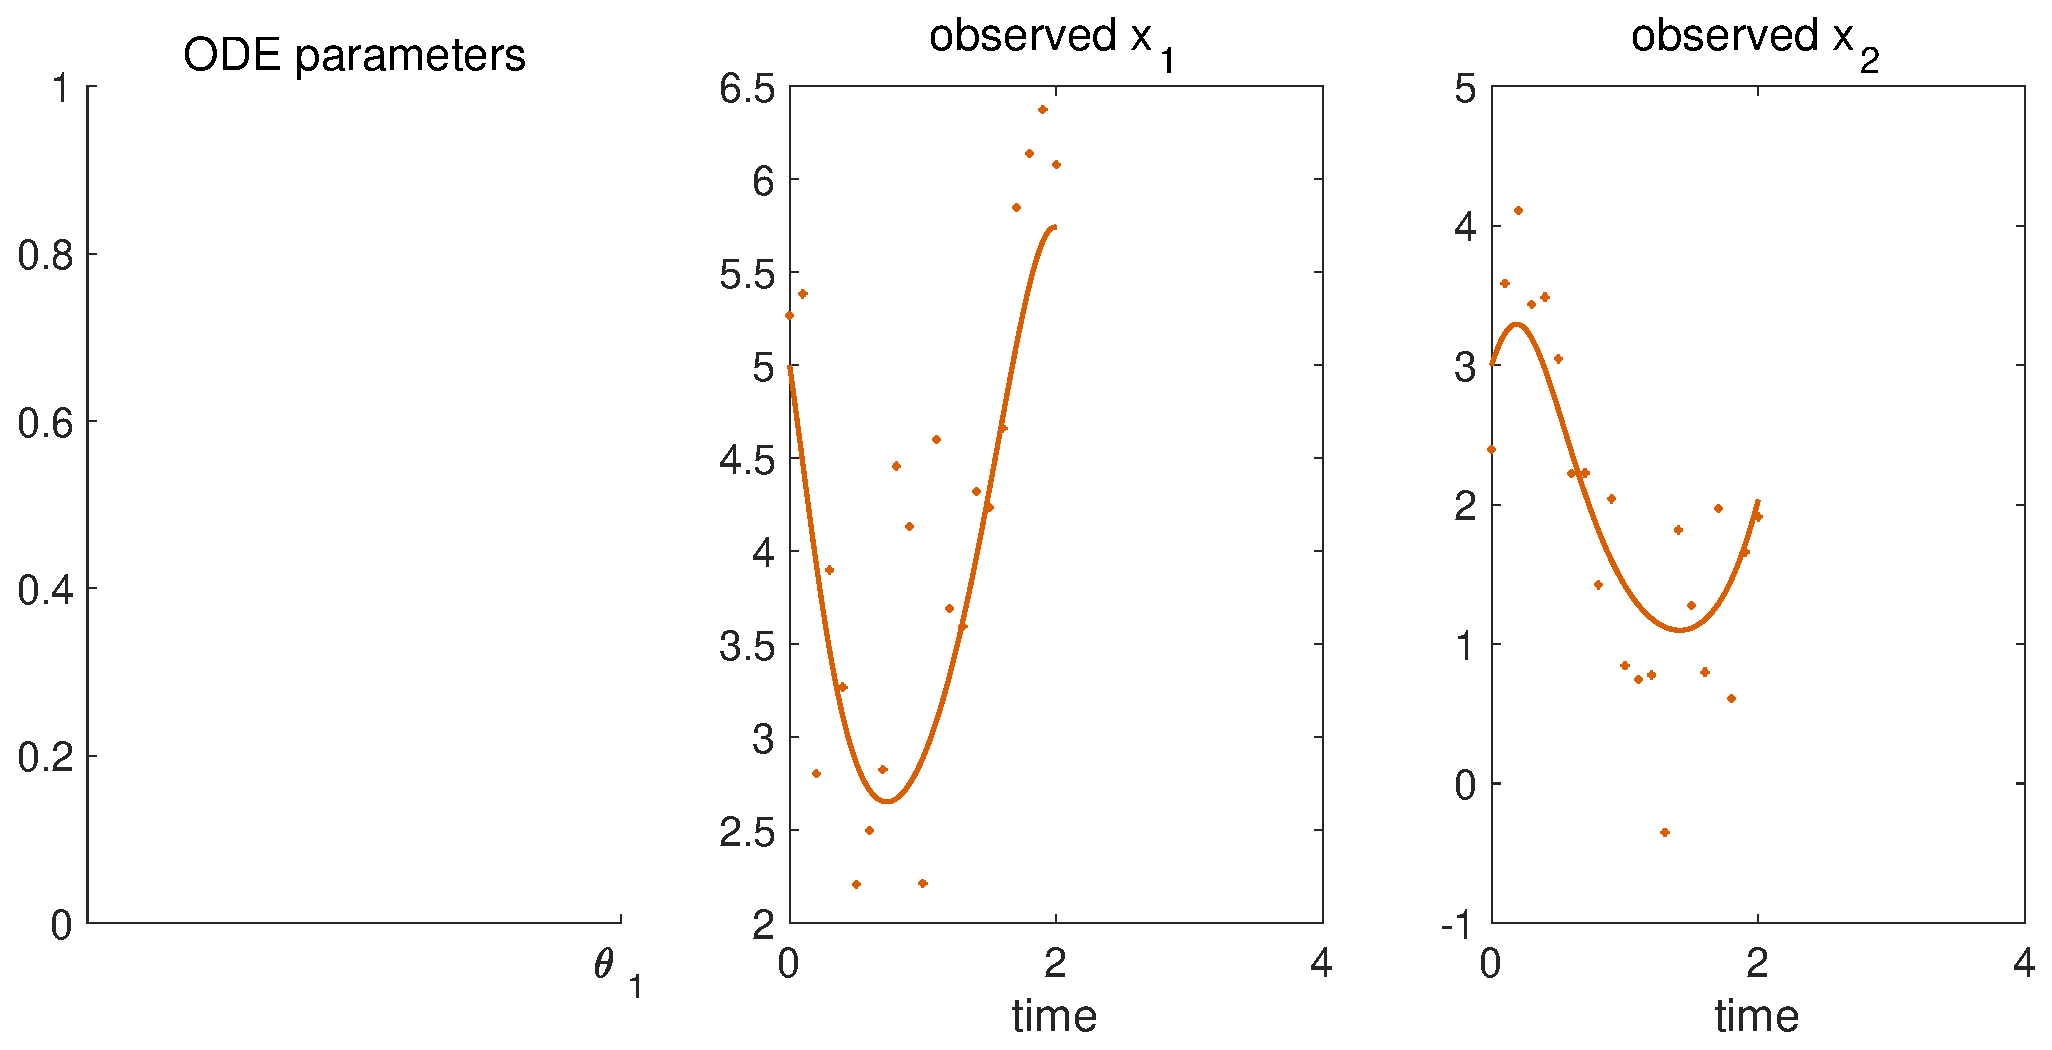
\includegraphics [width=5in]{VGM_for_Lotka_Volterra_01.eps}

}
\begin{par}
start timer
\end{par} \vspace{1em}
\color{RoyalPurple}\begin{verbatim}
tic;
\end{verbatim}
\color{black}


\section{Prior on States and State Derivatives}

\begin{par}
Gradient matching with Gaussian processes assumes a joint Gaussian process prior on states and their derivatives:
\end{par} \vspace{1em}
\begin{par}
$\left(\begin{array}{c} \mathbf{X} \\ \dot{\mathbf{X}} \end{array}\right) \sim \mathcal{N} \left(\begin{array}{c} \mathbf{X} \\ \dot{\mathbf{X}} \end{array}~;~\begin{array}{c} \mathbf{0} \\\mathbf{0} \end{array}~,~\begin{array}{cc} \mathbf{C}_{\boldsymbol\phi} & \mathbf{C}_{\boldsymbol\phi}' \\ '\mathbf{C}_\boldsymbol{\phi} & \mathbf{C}_{\boldsymbol\phi}'' \end{array} \right) \qquad (3)$,
\end{par} \vspace{1em}
\begin{par}
with
\end{par} \vspace{1em}
\begin{par}
$\mathrm{cov}(x_k(t), x_k(t)) = C_{\boldsymbol\phi_k}(t,t')$,
\end{par} \vspace{1em}
\begin{par}
$\mathrm{cov}(\dot{x}_k(t), x_k(t)) = \frac{\partial C_{\boldsymbol{\phi}_k}(t,t')}{\partial t} =: C_{{\boldsymbol\phi}_k}'(t,t')$,
\end{par} \vspace{1em}
\begin{par}
$\mathrm{cov}(x_k(t), \dot{x}_k(t)) = \frac{\partial C_{\boldsymbol\phi_k}(t,t')}{\partial t'} =: {'C_{\boldsymbol\phi_k}(t,t')}$,
\end{par} \vspace{1em}
\begin{par}
$\mathrm{cov}(\dot{x}_k(t), \dot{x}_k(t)) = \frac{\partial C_{\boldsymbol\phi_k}(t,t') }{\partial t \partial t'} =: C_{\boldsymbol\phi_k}''(t,t')$.
\end{par}


\section{Matching Gradients}

\begin{par}
Given the joint distribution over states and their derivatives (3) as well as the ODEs (2), we therefore have two expressions for the state derivatives:
\end{par} \vspace{1em}
\begin{par}
$\dot{\mathbf{X}} = \mathbf{F} + \boldsymbol\epsilon_1, \boldsymbol\epsilon_1 \sim\mathcal{N}\left(\boldsymbol\epsilon_1;\mathbf{0}, \mathbf{I}\gamma \right)$,
\end{par} \vspace{1em}
\begin{par}
$\dot{\mathbf{X}} = {'\mathbf{C}_{\boldsymbol\phi}} \mathbf{C}_{\boldsymbol\phi}^{-1}~\mathbf{X} + \boldsymbol\epsilon_2, \boldsymbol\epsilon_2 \sim\mathcal{N}\left(\boldsymbol\epsilon_2;\mathbf{0}, \mathbf{A} \right)$,
\end{par} \vspace{1em}
\begin{par}
where $\mathbf{F} := \mathbf{f}(\mathbf{X},\boldsymbol\theta)$ and $\mathbf{A} :=\mathbf{C}_{\boldsymbol\phi}'' -  {'\mathbf{C}_{\boldsymbol\phi}} \mathbf{C}_{\boldsymbol\phi}^{-1}\mathbf{C}_{\boldsymbol\phi}'$ and $\gamma$ is the error variance in the ODEs. Note that, in a deterministic system, the output of the ODEs $\mathbf{F}$ should equal the state derivatives $\dot{\mathbf{X}}$. However, in the first equation above we relax this constraint by adding stochasticity to the state derivatives $\dot{\mathbf{X}}$ in order to compensate for a potential model mismatch. The second equation above is obtained by deriving the conditional distribution for $\dot{\mathbf{X}}$ from the joint distribution in equation (3). Equating the two expressions in the equations above we can eliminate the unknown state derivatives $\dot{\mathbf{X}$:
\end{par} \vspace{1em}
\begin{par}
$\mathbf{F} = {'\mathbf{C}_{\boldsymbol\phi}} \mathbf{C}_{\boldsymbol\phi}^{-1} ~\mathbf{X} +\boldsymbol\epsilon_0 \qquad (4)$,
\end{par} \vspace{1em}
\begin{par}
with $\boldsymbol{\epsilon}_0 := \boldsymbol{\epsilon}_2 - \boldsymbol{\epsilon}_1$.
\end{par} \vspace{1em}
\color{RoyalPurple}\begin{verbatim}
[dC_times_invC,inv_C,A_plus_gamma_inv] = kernel_function(kernel,state,time.est);
\end{verbatim}
\color{black}


\section{Rewrite ODEs as Linear Combination in Parameters}

\begin{par}
Since, according to the mass action dynamics (equation 2), the ODEs are \textit{linear in the parameters} $\boldsymbol\theta$ we can rewrite the ODEs in equation (2) as a linear combination in the parameters:
\end{par} \vspace{1em}
\begin{par}
$\mathbf{B}_{\boldsymbol{\theta} k} \boldsymbol{\theta} + \mathbf{b}_{\boldsymbol{\theta} k} \stackrel{!}{=}\mathbf{f}_k(\mathbf{X},\boldsymbol{\theta}) \qquad (5)$,
\end{par} \vspace{1em}
\begin{par}
where matrices $\mathbf{B}_{\boldsymbol{\theta} k}$ and $\mathbf{b}_{\boldsymbol{\theta} k}$ are defined such that the ODEs $\mathbf{f}_k(\mathbf{X},\boldsymbol{\theta})$ are expressed as a linear combination in $\boldsymbol{\theta}$.
\end{par} 
\color{RoyalPurple}\begin{verbatim}
[ode_param.lin_comb.B,ode_param.lin_comb.b] = ...
rewrite_odes_as_linear_combination_in_parameters(ode,symbols);
\end{verbatim}
\color{black}


\section{Posterior over ODE Parameters}

\begin{par}
Inserting (5) into (4) and solving for $\boldsymbol{\theta}$ yields:
\end{par} \vspace{1em}
\begin{par}
$\boldsymbol{\theta} = \mathbf{B}_{\boldsymbol{\theta}}^+ \left( {'\mathbf{C}_{\boldsymbol{\phi}}}\mathbf{C}_{\boldsymbol{\phi}}^{-1} \mathbf{X} - \mathbf{b}_{\boldsymbol{\theta}} + \boldsymbol{\epsilon}_0\right)$,
\end{par} \vspace{1em}
\begin{par}
where $\mathbf{B}_{\boldsymbol{\theta}}^+$ denotes the pseudo-inverse of $\mathbf{B}_{\boldsymbol{\theta}}$. Since $\mathbf{C}_{\boldsymbol{\phi}}$ is block diagonal we can rewrite the expression above as:
\end{par} \vspace{1em}
\begin{par}
$\boldsymbol{\theta} = \left( \mathbf{B}_{\boldsymbol{\theta}}^T \mathbf{B}_{\boldsymbol{\theta}} \right)^{-1} ~\mathbf{B}_{\boldsymbol{\theta}}^T  \left( \sum_k {'\mathbf{C}_{\boldsymbol{\phi}_k}}\mathbf{C}_{\boldsymbol{\phi}_k}^{-1} \mathbf{X}_k - \mathbf{b}_{\boldsymbol{\theta} k} + \boldsymbol{\epsilon}_0^{(k)} \right)\\ ~= \left( \mathbf{B}_{\boldsymbol{\theta}}^T \mathbf{B}_{\boldsymbol{\theta}} \right)^{-1} \left(\sum_k \mathbf{B}_{\boldsymbol{\theta} k}^T \left( {'\mathbf{C}_{\boldsymbol{\phi}_k}}\mathbf{C}_{\boldsymbol{\phi}_k}^{-1} \mathbf{X}_k - \mathbf{b}_{\boldsymbol{\theta} k} +\boldsymbol{\epsilon}_0^{(k)} \right) \right)$,
\end{par} \vspace{1em}
\begin{par}
where we subsitute the Moore-Penrose inverse for the pseudo-inverse (i.e. $\mathbf{B}_{\boldsymbol{\theta}}^+ := \left( \mathbf{B}_{\boldsymbol{\theta}}^T \mathbf{B}_{\boldsymbol{\theta}}\right)^{-1} \mathbf{B}_{\boldsymbol{\theta}}^T$). We can therefore derive the posterior distribution over ODE parameters:
\end{par} \vspace{1em}
\begin{par}
$p(\boldsymbol{\theta} \mid \mathbf{X}, \boldsymbol{\phi}, \gamma) = \mathcal{N}\left(\boldsymbol{\theta} ; \left( \mathbf{B}_{\boldsymbol{\theta}}^T\mathbf{B}_{\boldsymbol{\theta}} \right)^{-1} \left( \sum_k \mathbf{B}_{\boldsymbol{\theta} k}^T ~\left( {'\mathbf{C}_{\boldsymbol{\phi} k}} \mathbf{C}_{\boldsymbol{\phi} k}^{-1} \mathbf{X}_k -\mathbf{b}_{\boldsymbol{\theta} k} \right) \right), ~ \mathbf{B}_{\boldsymbol{\theta}}^+ ~(\mathbf{A} + \mathbf{I}\gamma) ~ \mathbf{B}_{\boldsymbol{\theta}}^{+T}\right) \qquad (6)$.
\end{par} \vspace{1em}


\section{Rewrite ODEs as Linear Combination in Individual States}

\begin{par}
Since, according to the mass action dynamics (equation 2), the ODEs are \textit{linear in the individual state} $\mathbf{x}_u$ we can rewrite the ODE $\mathbf{f}_k(\mathbf{X},\boldsymbol\theta)$ as a linear combination in the individual state $\mathbf{x}_u$:
\end{par} \vspace{1em}
\begin{par}
$\mathbf{R}_{uk} \mathbf{x}_u + \mathbf{r}_{uk} \stackrel{!}{=}\mathbf{f}_k(\mathbf{X},\boldsymbol{\theta})$,
\end{par} \vspace{1em}
\begin{par}
where matrices  $\mathbf{R}_{uk}$ and  $\mathbf{r}_{uk}$ are defined such that the ODE $\mathbf{f}_k(\mathbf{X},\boldsymbol{\theta})$ is expressed as a linear combination in the individual state $\mathbf{x}_u$.
\end{par} \vspace{1em}
\color{RoyalPurple}\begin{verbatim}
[state.lin_comb.R,state.lin_comb.r] = ...
rewrite_odes_as_linear_combination_in_ind_states(ode,symbols,coupling_idx.states);
\end{verbatim}
\color{black}


\section{Posterior over Individual States}

\begin{par}
Given the linear combination of the ODEs w.r.t. an individual state, we define the matrices $\mathbf{B}_u$ and $\mathbf{b}_u$ such that the expression $\mathbf{f}(\mathbf{X},\boldsymbol{\theta}) - {'\mathbf{C}}_{\boldsymbol{\phi}}\mathbf{C}_{\boldsymbol{\phi}}^{-1} \mathbf{X}$ is rewritten as a linear combination in an individual state $\mathbf{x}_u$:
\end{par} \vspace{1em}
\begin{par}
$\mathbf{B}_{u} \mathbf{x}_u + \mathbf{b}_{u} \stackrel{!}{=}\mathbf{f}(\mathbf{X},\boldsymbol{\theta}) - {'\mathbf{C}}_{\boldsymbol{\phi}}\mathbf{C}_{\boldsymbol{\phi}}^{-1} \mathbf{X} \qquad (7)$.
\end{par} \vspace{1em}
\begin{par}
Inserting (7) into (4) and solving for $\mathbf{x}_u$ yields:
\end{par} \vspace{1em}
\begin{par}
$\mathbf{x}_u = \mathbf{B}_{u}^+ \left( \boldsymbol{\epsilon}_0 -\mathbf{b}_{u}\right)$,
\end{par} \vspace{1em}
\begin{par}
where $\mathbf{B}_{u}^+$ denotes the pseudo-inverse of $\mathbf{B}_{u}$. Since $\mathbf{C}_{\boldsymbol{\phi}}$ is block diagonal we can rewrite the expression above as:
\end{par} \vspace{1em}
\begin{par}
$\mathbf{x}_u = \left( \mathbf{B}_{u} \mathbf{B}_{u}^T \right)^{-1}\mathbf{B}_{u}^T \sum_k \left(\boldsymbol{\epsilon}_0^{(k)} -\mathbf{b}_{uk} \right)\\ \quad= \left( \mathbf{B}_{u} \mathbf{B}_{u}^T \right)^{-1} \sum_k\mathbf{B}_{uk}^T \left(\boldsymbol{\epsilon}_0^{(k)} -\mathbf{b}_{uk} \right)$,
\end{par} \vspace{1em}
\begin{par}
where we substitute the Moore-Penrose inverse for the pseudo-inverse (i.e. $\mathbf{B}_{\boldsymbol{\theta}}^+ := \left( \mathbf{B}_{\boldsymbol{\theta}}^T \mathbf{B}_{\boldsymbol{\theta}}\right)^{-1} \mathbf{B}_{\boldsymbol{\theta}}^T$).  We can therefore derive the posterior distribution over an individual state $\mathbf{x}_{u}$:
\end{par} \vspace{1em}
\begin{par}
$p(\mathbf{x}_u \mid \mathbf{X}_{-u}, \boldsymbol{\phi}, \gamma)= \mathcal{N}\left(\mathbf{x}_u ; \left( \mathbf{B}_{u} \mathbf{B}_{u}^T\right)^{-1} \left( - \sum_k \mathbf{B}_{uk}^T \mathbf{b}_{uk} \right),~\mathbf{B}_{u}^{+} ~ (\mathbf{A} + \mathbf{I}\gamma) ~ \mathbf{B}_u^{+T}\right) \qquad (8)$,
\end{par} \vspace{1em}
\begin{par}
with $\mathbf{X}_{-u}$ denoting the set of all states except state $\mathbf{x}_u$.
\end{par} \vspace{1em}


\section{Mean-field Variational Inference}

\begin{par}
To infer the parameters $\boldsymbol{\theta}$, we want to find the maximum a posteriori estimate (MAP):
\end{par} \vspace{1em}
\begin{par}
$\boldsymbol{\theta}^* := \mathrm{arg} \max_{\boldsymbol{\theta}} ~ \ln p(\boldsymbol{\theta} \mid\mathbf{Y},\boldsymbol{\phi},\gamma,\mathbf \sigma)\\ \quad= \mathrm{arg}\max_{\boldsymbol{\theta}} ~ \ln \int  p(\boldsymbol{\theta},\mathbf{X} \mid\mathbf{Y},\boldsymbol{\phi},\gamma,\boldsymbol\sigma) d\mathbf{X}\\ \quad= \mathrm{arg}\max_{\boldsymbol{\theta}} ~ \ln \int p(\boldsymbol{\theta} \mid \mathbf{X},\boldsymbol{\phi},\gamma)p(\mathbf{X} \mid \mathbf{Y}, \boldsymbol{\phi},\boldsymbol\sigma) d\mathbf{X} \qquad(9)$.
\end{par} \vspace{1em}
\begin{par}
However, the integral above is intractable due to the strong couplings induced by the nonlinear ODEs $\mathbf{f}$ which appear in the term $p(\boldsymbol{\theta} \mid \mathbf{X},\boldsymbol{\phi},\gamma)$.
\end{par} \vspace{1em}
\begin{par}
We use mean-field variational inference to establish variational lower bounds that are analytically tractable by decoupling state variables from the ODE parameters as well as decoupling the state variables from each other. Note that, since the ODEs described by equation (2) are \textit{locally linear}, both conditional distributions $p(\boldsymbol{\theta} \mid\mathbf{X},\mathbf{Y},\boldsymbol{\phi},\gamma,\boldsymbol\sigma)$ (equation (6)) and $p(\mathbf{x}_u \mid \boldsymbol{\theta},\mathbf{X}_{-u},\mathbf{Y},\boldsymbol{\phi},\gamma,\boldsymbol\sigma)$ (equation (8)) are analytically tractable and Gaussian distributed as mentioned previously. The decoupling is induced by designing a variational distribution $Q(\boldsymbol{\theta},\mathbf{X})$ which is restricted to the family of factorial distributions:
\end{par} \vspace{1em}
\begin{par}
$\mathcal{Q} := \bigg{\{} Q : Q(\boldsymbol{\theta},\mathbf{X}) = q(\boldsymbol{\theta}) \prod_uq(\mathbf{x}_u) \bigg{\}}$.
\end{par} \vspace{1em}
\begin{par}
The particular form of $q(\boldsymbol{\theta})$ and $q(\mathbf{x}_u)$ are designed to be Gaussian distributed which places them in the same family as the true full conditional distributions. To find the optimal factorial distribution we minimize the Kullback-Leibler divergence between the variational and the true posterior distribution:
\end{par} \vspace{1em}
\begin{par}
$\hat{Q} := \mathrm{arg} \min_{Q(\boldsymbol{\theta},\mathbf{X}) \in \mathcal{Q}} \mathrm{KL}\left[ Q(\boldsymbol{\theta},\mathbf{X}) \mid \mid p(\boldsymbol{\theta},\mathbf{X} \mid\mathbf{Y},\boldsymbol{\phi}, \gamma,\mathbf\boldsymbol{\sigma}) \right] \qquad (10)$,
\end{par} \vspace{1em}
\begin{par}
where $\hat{Q}$ is the proxy distribution. The proxy distribution that minimizes the KL-divergence (10) depends on the true full conditionals and is given by:
\end{par} \vspace{1em}
\begin{par}
$\hat{q}({\boldsymbol{\theta}}) \propto \exp \left(~ E_{Q_{-\boldsymbol{\theta}}} \ln p(\boldsymbol{\theta} \mid\mathbf{X},\mathbf{Y},\boldsymbol{\phi},\gamma,\mathbf\boldsymbol{\sigma}) ~\right) \qquad (11)\\\hat{q}(\mathbf{x}_u) \propto \exp\left( ~ E_{Q_{-u}} \ln p(\mathbf{x}_u\mid \boldsymbol{\theta}, \mathbf{X}_{-u},\mathbf{Y},\boldsymbol{\phi},\gamma,\boldsymbol{\sigma}) ~ \right)\qquad (12)$.
\end{par} \vspace{1em}


\section{Fitting Observations of State Trajectories}

\begin{par}
We fit the observations of state trajectories by standard GP regression. The data-informed distribution $p(\mathbf{X} \mid \mathbf{Y}, \boldsymbol{\phi},\mathbf\boldsymbol{\sigma})$ in euqation (9) can be determined analytically using Gaussian process regression with the GP prior $p(\mathbf{X} \mid\boldsymbol{\phi}) = \prod_k \mathcal{N}(\mathbf{x}_k ;\mathbf{0},\mathbf{C}_{\boldsymbol{\phi}_k})$:
\end{par} \vspace{1em}
\begin{par}
$p(\mathbf{X} \mid \mathbf{Y}, \boldsymbol{\phi},\gamma) = \prod_k\mathcal{N}(\mathbf{x}_k ;\boldsymbol\mu_k(\mathbf{y}_k),\mathbf\boldsymbol{\sigma}_k)$,
\end{par} \vspace{1em}
\begin{par}
where $\boldsymbol\mu_k(\mathbf{y}_k) := \boldsymbol{\sigma}_k^{-2} \left(\boldsymbol{\sigma}_k^{-2}\mathbf{I} + \mathbf{C}_{\boldsymbol{\phi}_k}^{-1} \right)^{-1} \mathbf{y}_k$ and $\boldsymbol{\sigma}_k ^{-1}:=\boldsymbol{\sigma}_k^{-2} \mathbf{I} +\mathbf{C}_{\mathbf\boldsymbol{\phi}_k}^{-1}$.
\end{par} \vspace{1em}
\color{RoyalPurple}\begin{verbatim}
[mu,inv_sigma] = fitting_state_observations(inv_C,obs_to_state_relation,...
simulation,symbols);
\end{verbatim}
\color{black}


\section{Coordinate Ascent Variational Gradient Matching}

\begin{par}
We minimize the KL-divergence in equation (10) by coordinate descent (where each step is analytically tractable) by iterating between determining the proxy for the distribution over ODE parameters $\hat{q}(\boldsymbol{\theta})$ and the proxies for the distribution over individual states $\hat{q}(\mathbf{x}_u)$.
\end{par}

\vspace{1.5em}
\textbf{Initialize the state estimation by the GP regression posterior}

\color{RoyalPurple}\begin{verbatim}
state.proxy.mean = array2table([time.est',mu],...
'VariableNames',['time',symbols.state_string]);
\end{verbatim}
\color{black}
\begin{par}

\end{par} \vspace{1.5em}

\textbf{Coordinate ascent}

\color{RoyalPurple}\begin{verbatim}
for i = 1:opt_settings.coord_ascent_numb_iter
\end{verbatim}
\color{black}

\subsection{Proxy for ODE parameters}


\begin{par}
Expanding the proxy distribution in equation (11) for $\boldsymbol{\theta}$ yields:
\end{par} \vspace{1em}

\begin{par}
$\hat{q}(\mathbf{\boldsymbol\theta}) \propto \exp
\left( ~E_{Q_{-\boldsymbol\theta}}     \ln p(\boldsymbol\theta \mid \mathbf{X},\mathbf{Y},\boldsymbol\phi,\gamma,\boldsymbol\sigma)
~     \right) \\ \qquad= \exp \left( ~E_{Q_{-\boldsymbol{\theta}}} \ln \mathcal{N}\left(\boldsymbol{\theta}
; \left(    \mathbf{B}_{\boldsymbol{\theta}}^T \mathbf{B}_{\boldsymbol{\theta}} \right)^{-1}
\left( \sum_k    \mathbf{B}_{\boldsymbol{\theta} k}^T ~ \left( {'\mathbf{C}_{\boldsymbol{\phi}
k}}    \mathbf{C}_{\boldsymbol{\phi} k}^{-1} \mathbf{X}_k - \mathbf{b}_{\boldsymbol{\theta}
k} \right)    \right), ~ \mathbf{B}_{\boldsymbol{\theta}}^+ ~ (\mathbf{A} + \mathbf{I}\gamma)
~    \mathbf{B}_{\boldsymbol{\theta}}^{+T} \right) ~\right)$,
\end{par} \vspace{1em}

where we substitute $p(\boldsymbol{\theta} \mid \mathbf{X},\boldsymbol{\phi},\gamma)$ with its density given in equation (6).
    \color{RoyalPurple}\begin{verbatim}
             [param_proxy_mean,param_proxy_inv_cov] = ...
             proxy_for_ode_parameters(state.proxy.mean{:,symbols.state_string},...
                    dC_times_invC,ode_param.lin_comb,symbols,A_plus_gamma_inv,opt_settings);
\end{verbatim}
\color{black}
\begin{par}
Intermediate results
\end{par} \vspace{1em}
\color{RoyalPurple}\begin{verbatim}
            if i==1 || ~mod(i,1)
                plot_results(fig_handle,state.proxy,simulation,param_proxy_mean,...
                plot_handle,symbols,plot_settings,'not_final');
            end
\end{verbatim}
\color{black}

{\centering
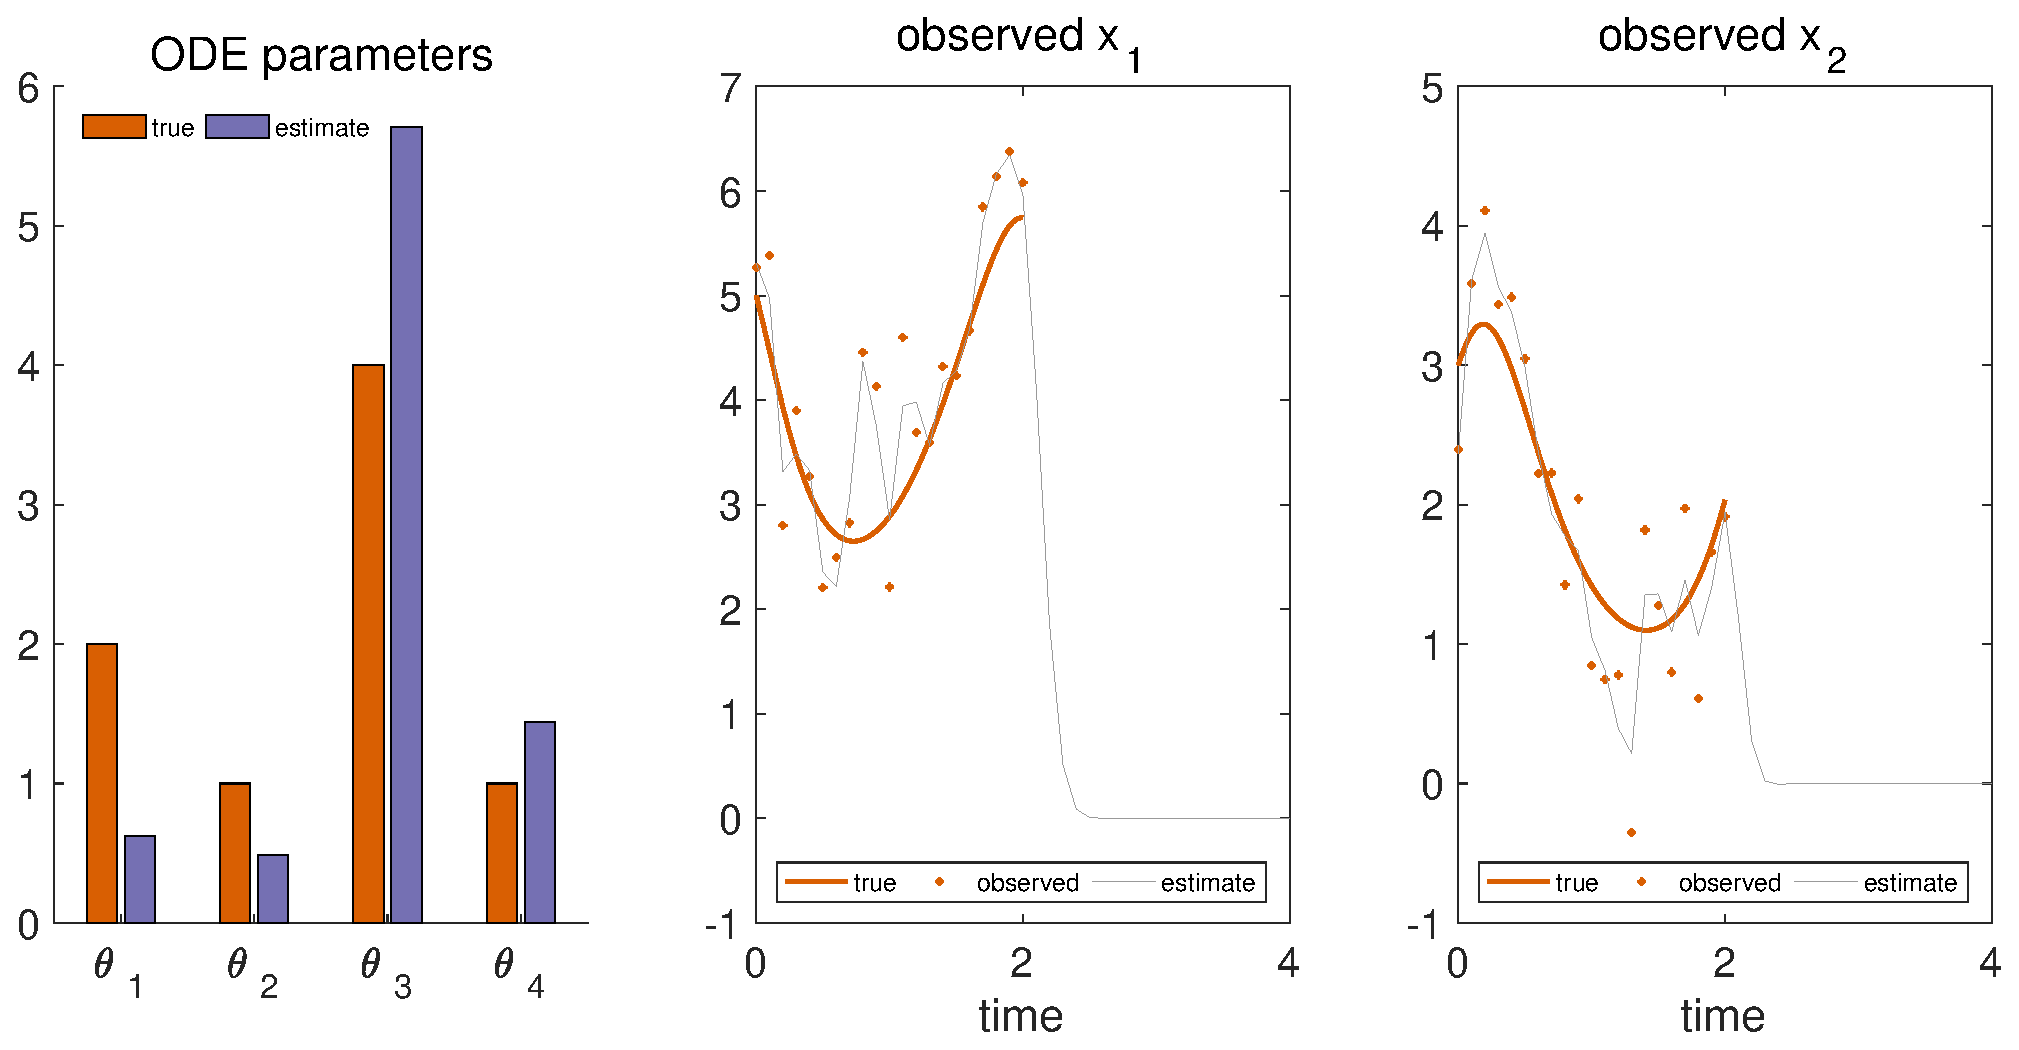
\includegraphics [width=5in]{VGM_for_Lotka_Volterra_02.eps}

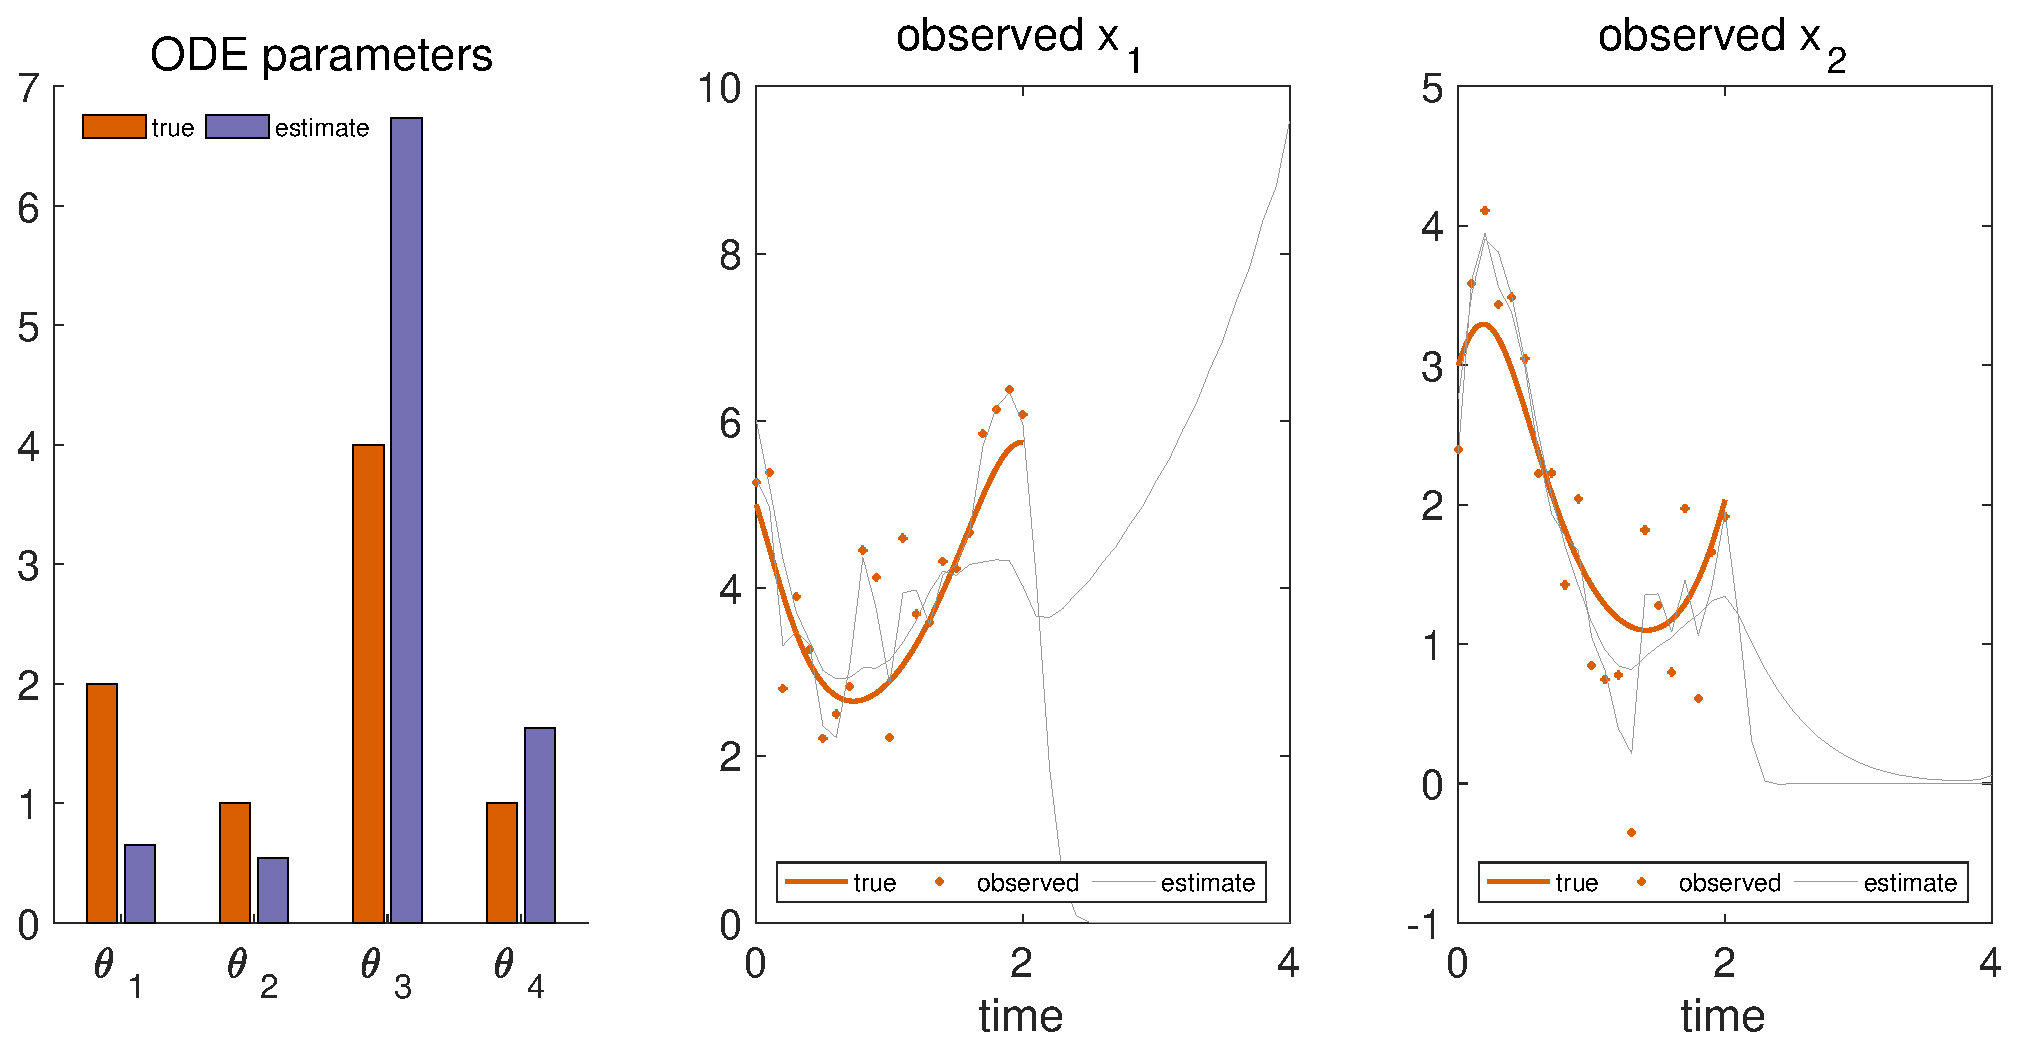
\includegraphics [width=5in]{VGM_for_Lotka_Volterra_03.eps}

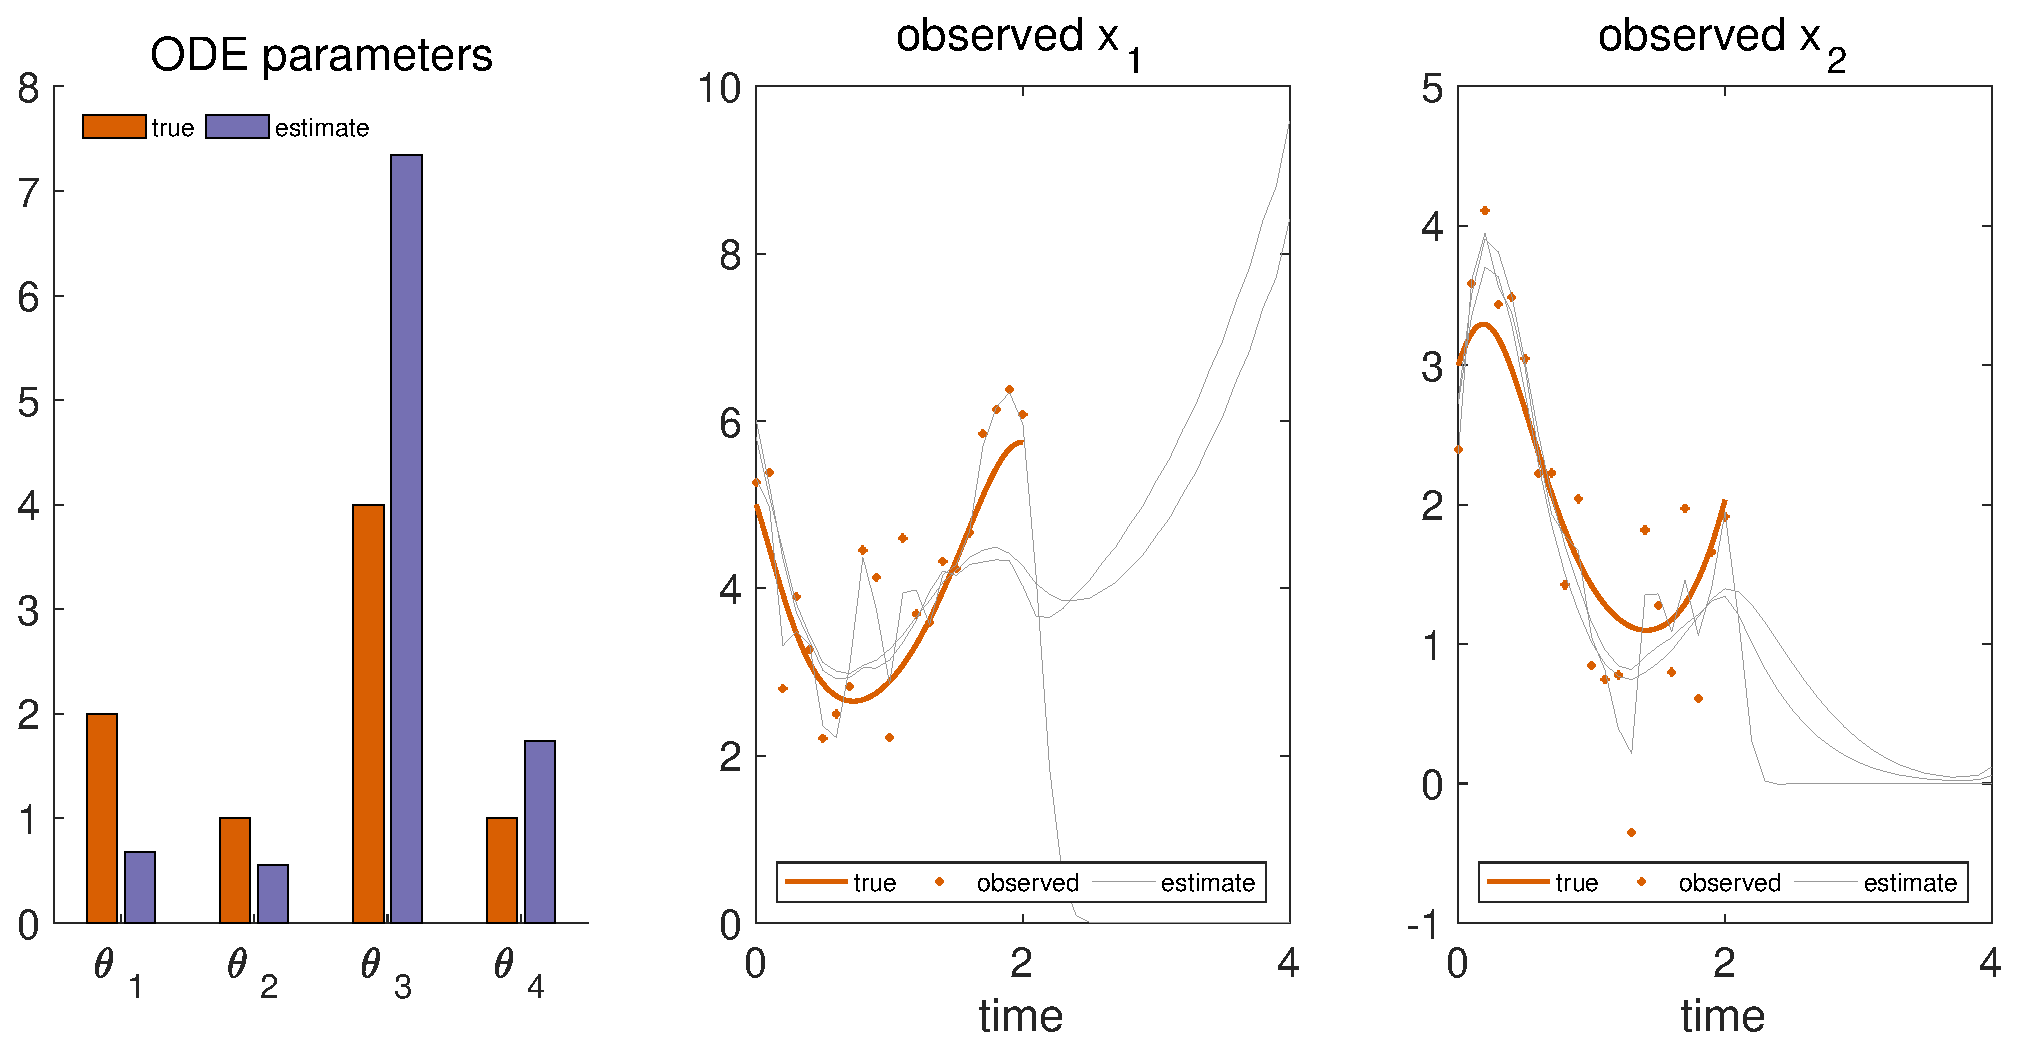
\includegraphics [width=5in]{VGM_for_Lotka_Volterra_04.eps}

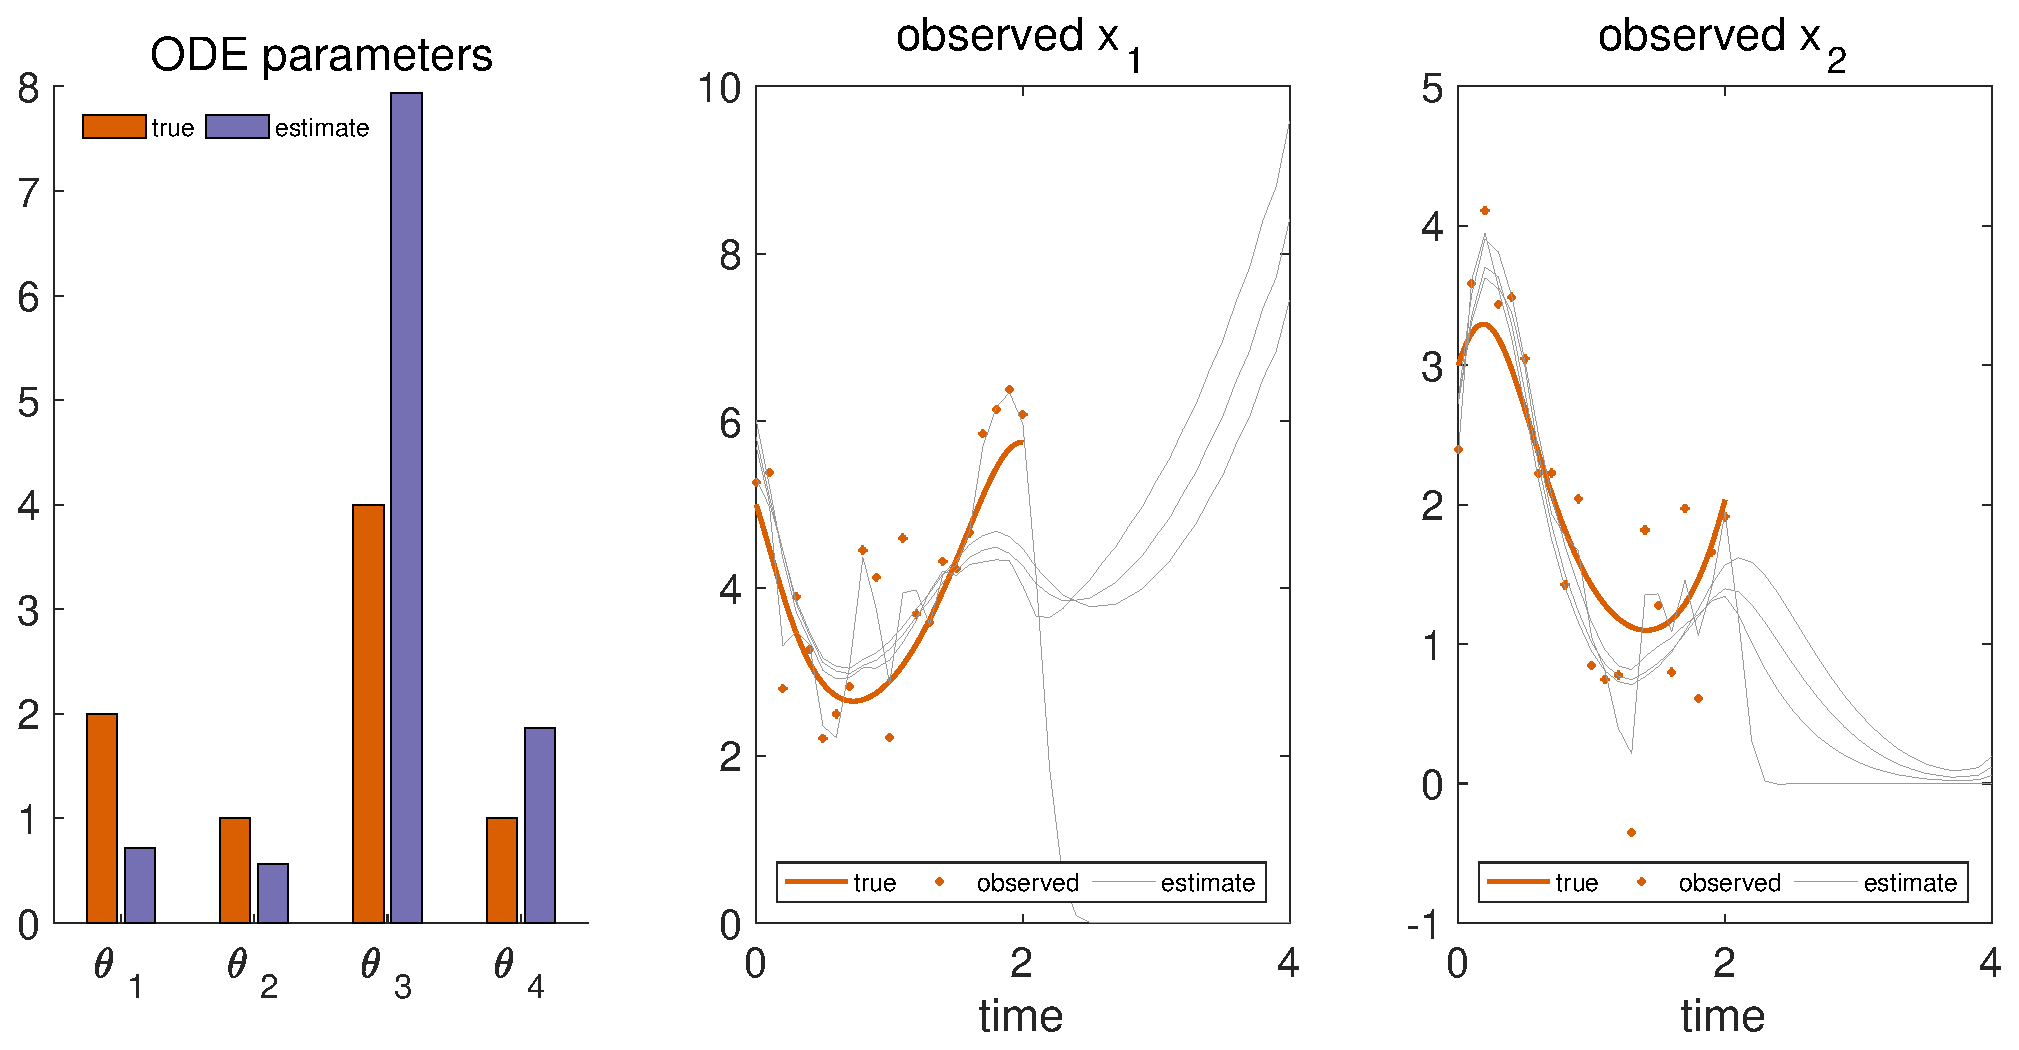
\includegraphics [width=5in]{VGM_for_Lotka_Volterra_05.eps}

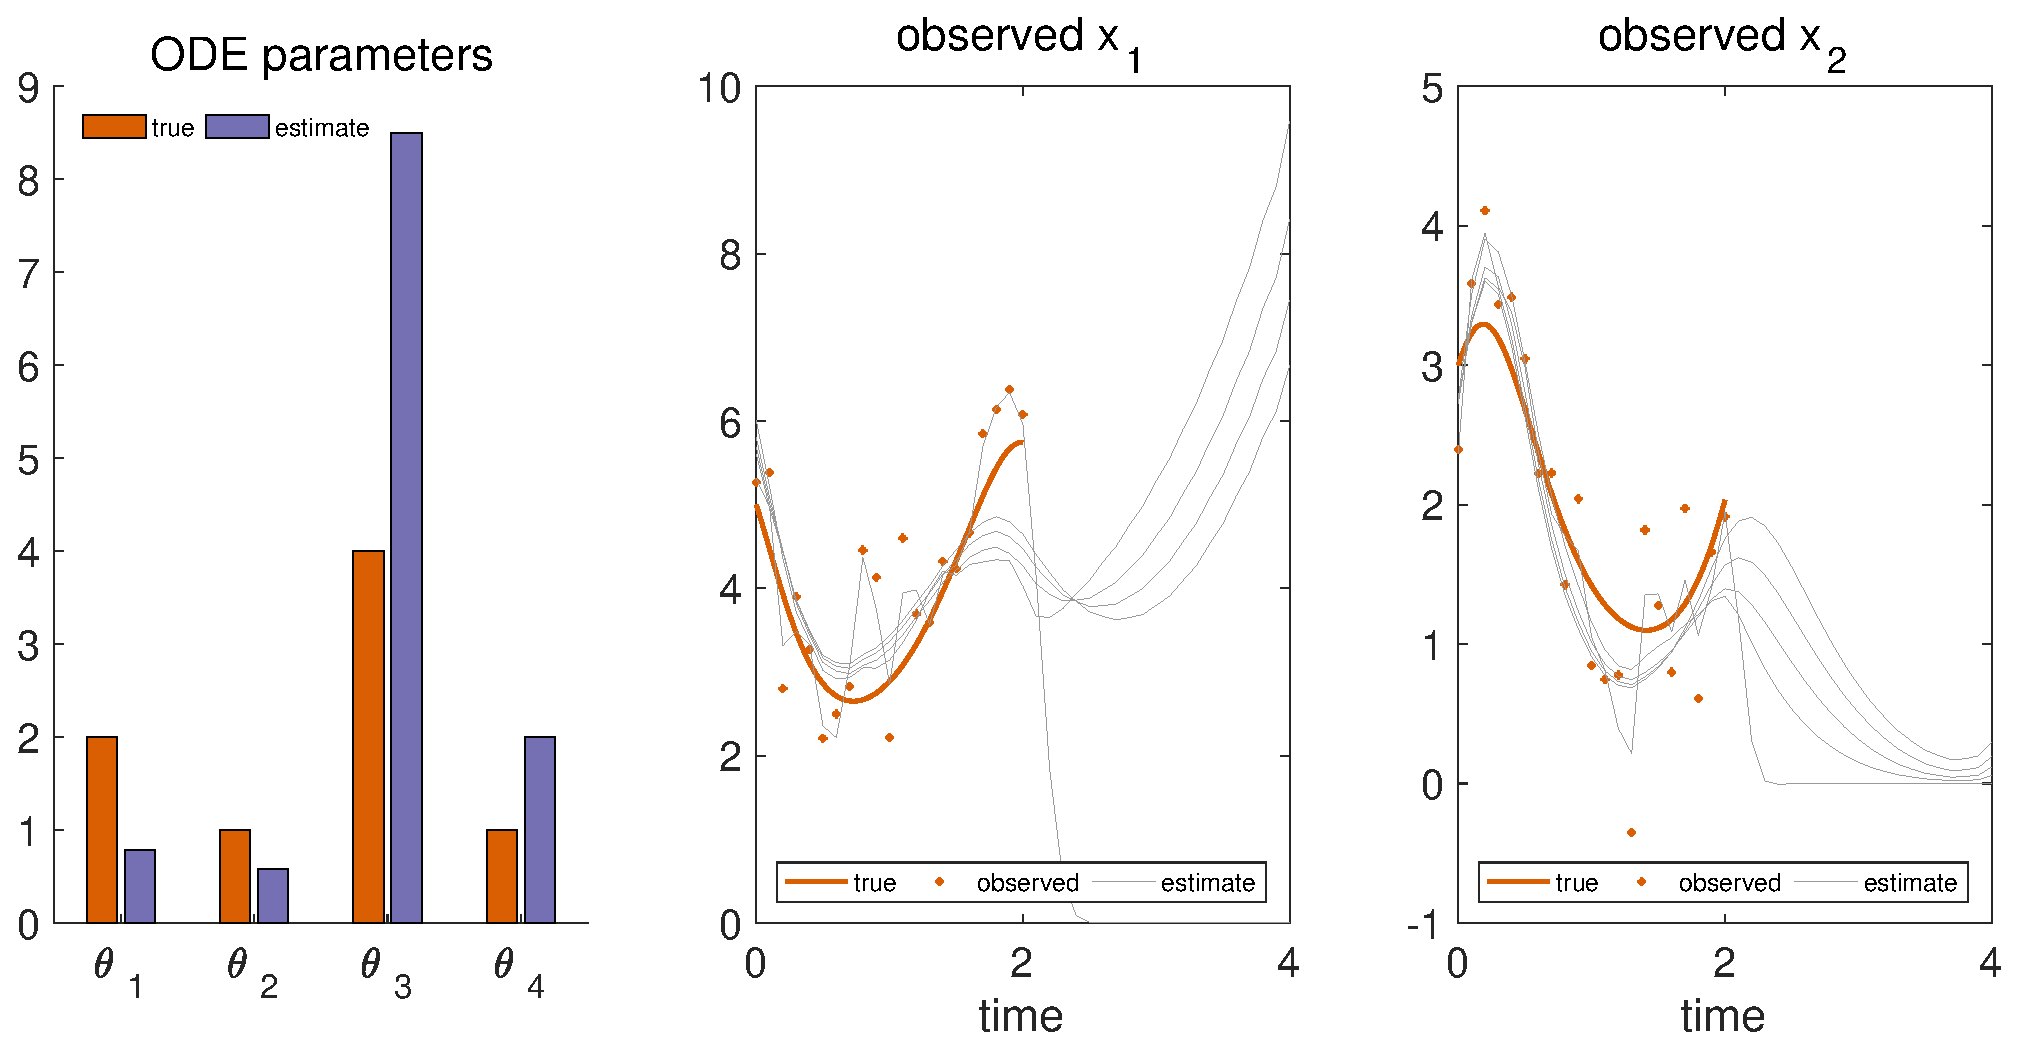
\includegraphics [width=5in]{VGM_for_Lotka_Volterra_06.eps}

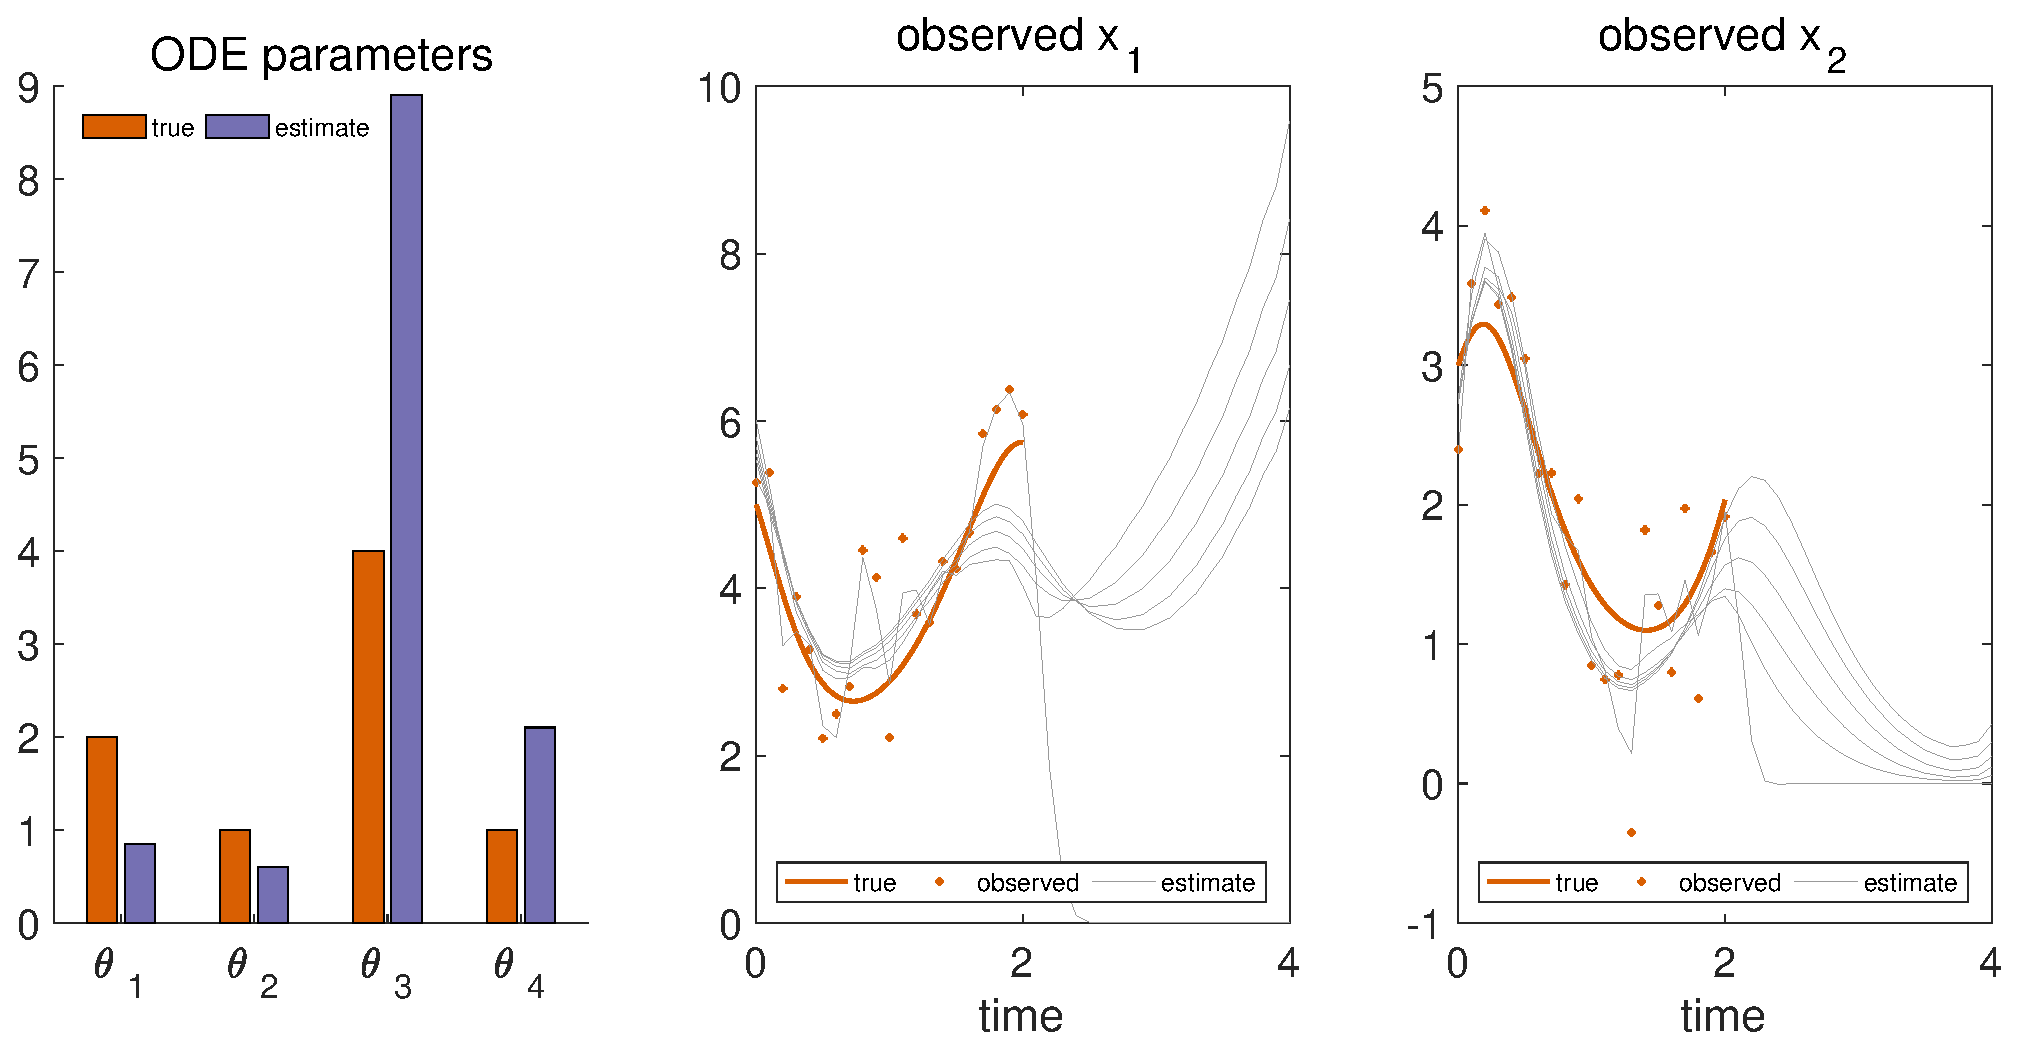
\includegraphics [width=5in]{VGM_for_Lotka_Volterra_07.eps}

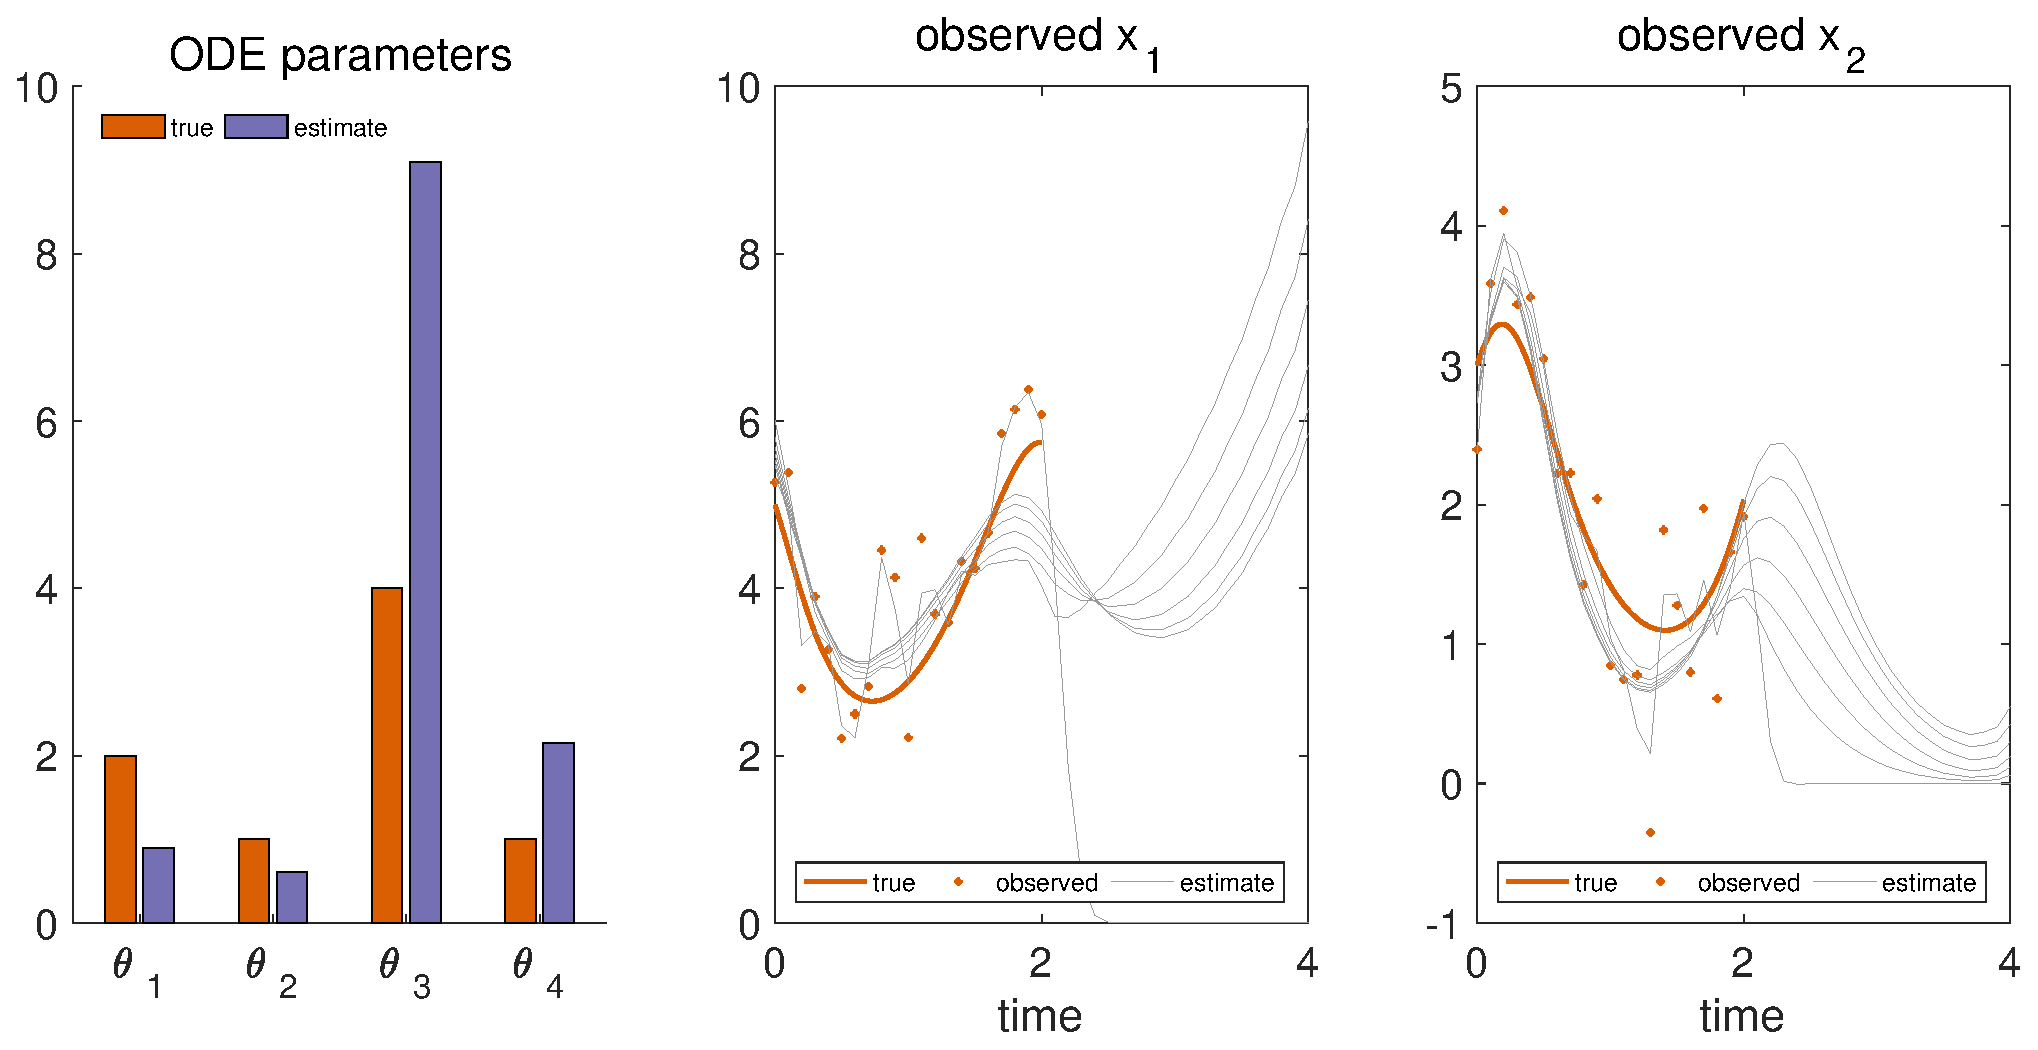
\includegraphics [width=5in]{VGM_for_Lotka_Volterra_08.eps}

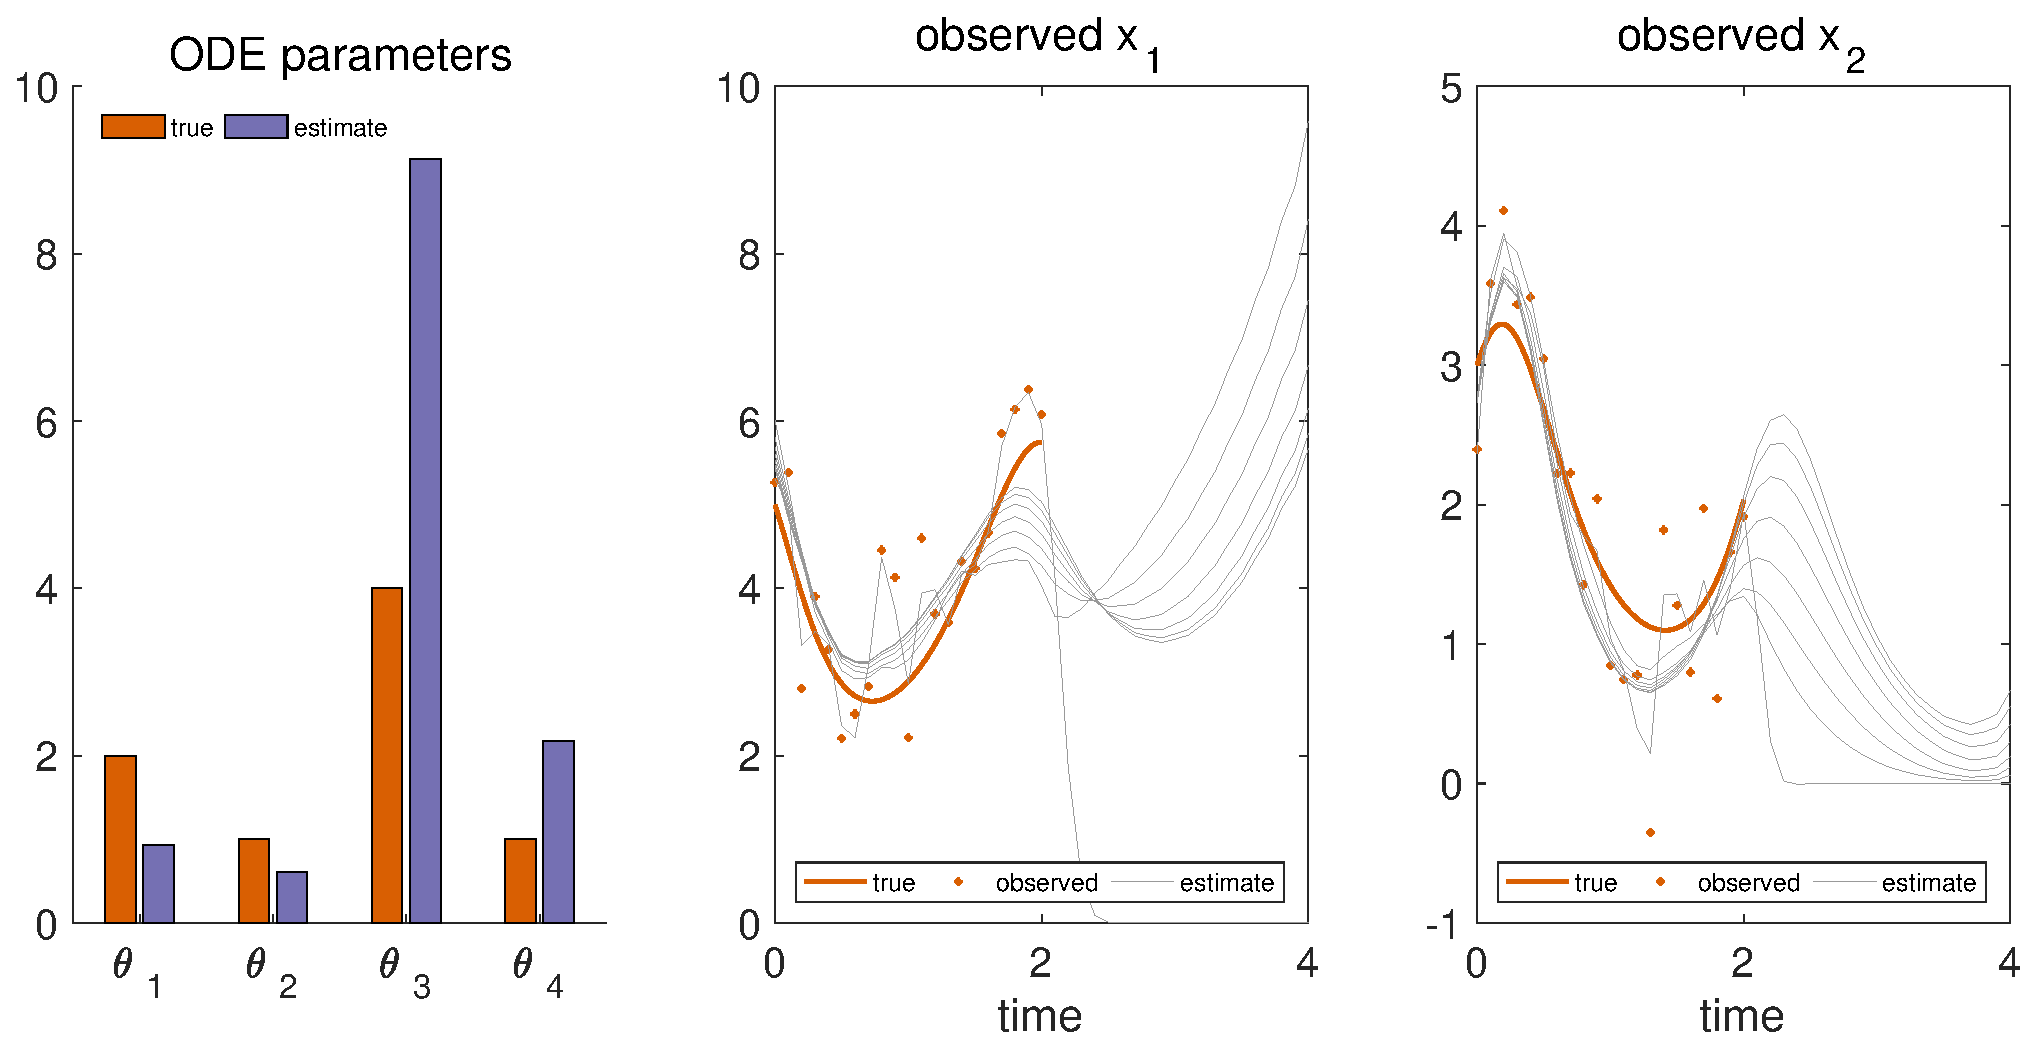
\includegraphics [width=5in]{VGM_for_Lotka_Volterra_09.eps}

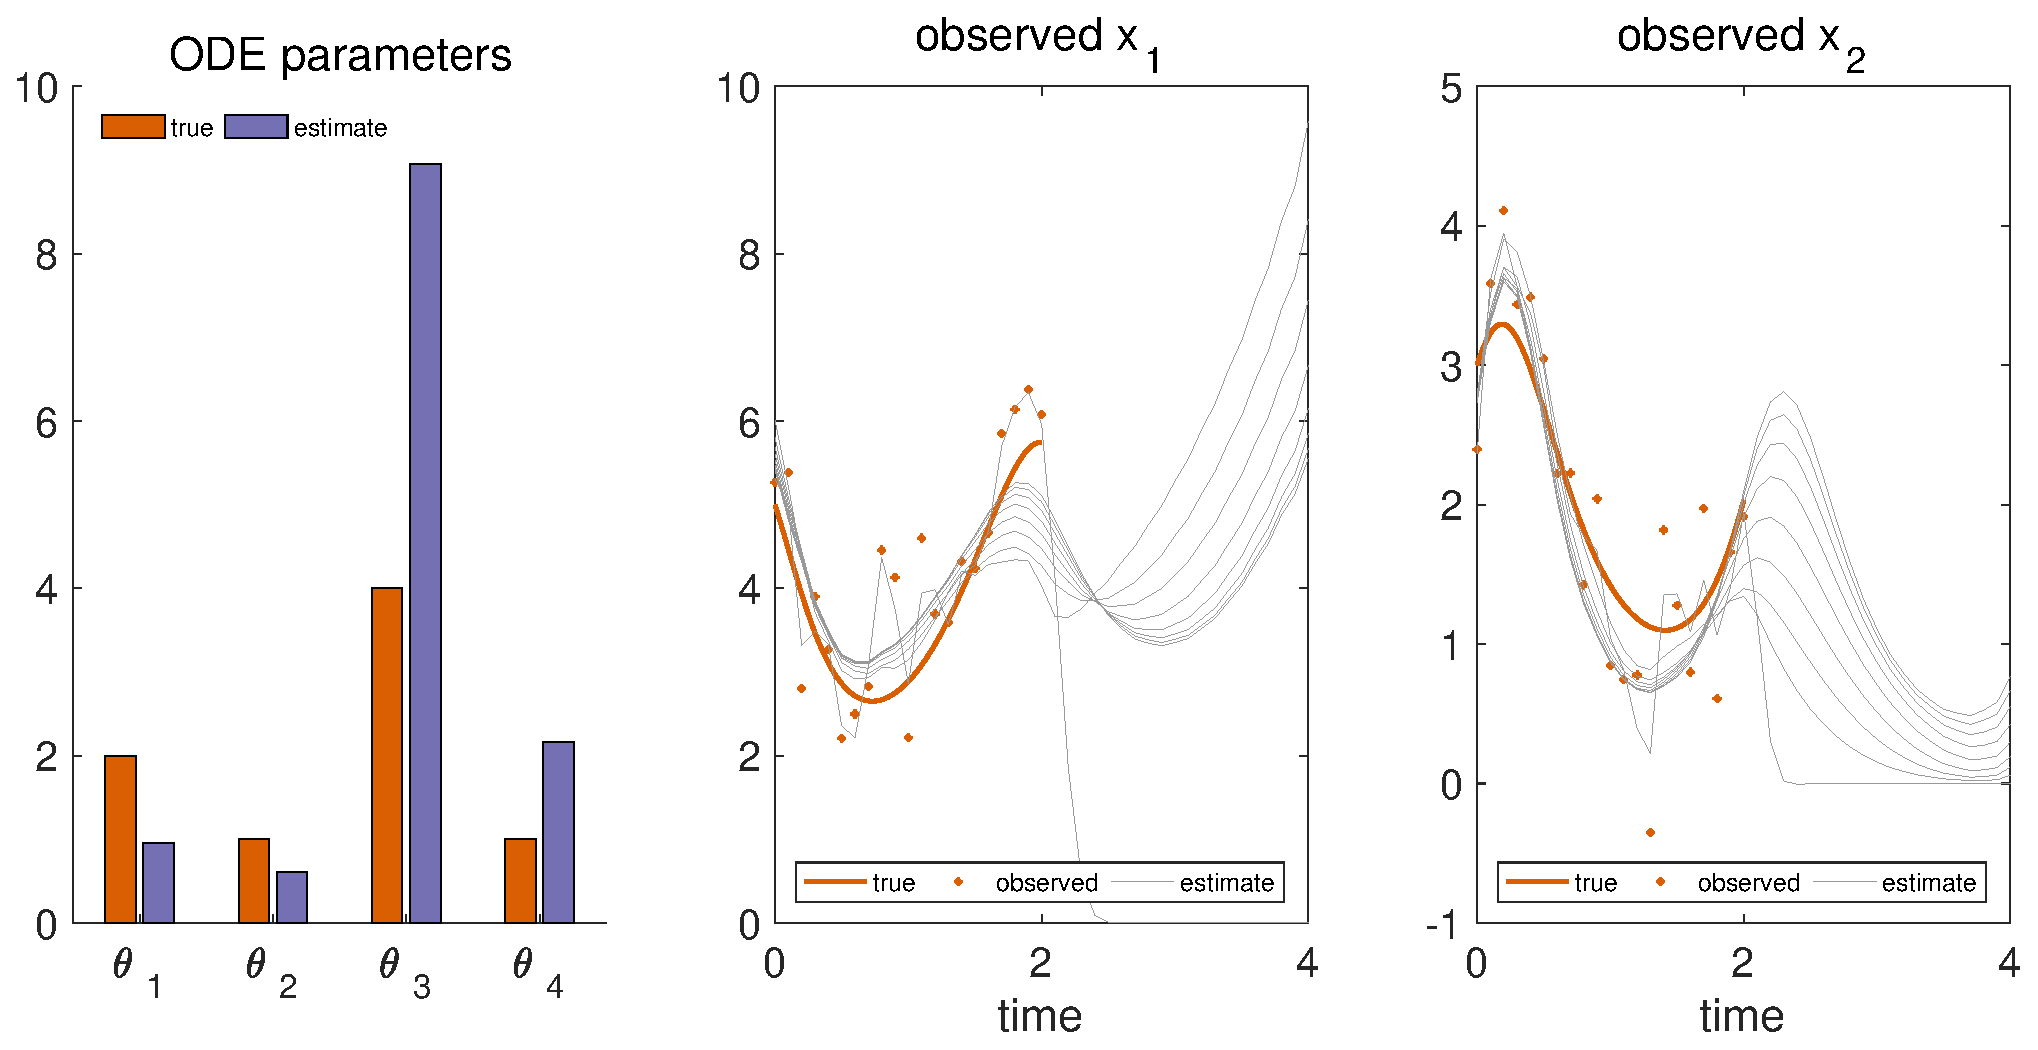
\includegraphics [width=5in]{VGM_for_Lotka_Volterra_10.eps}

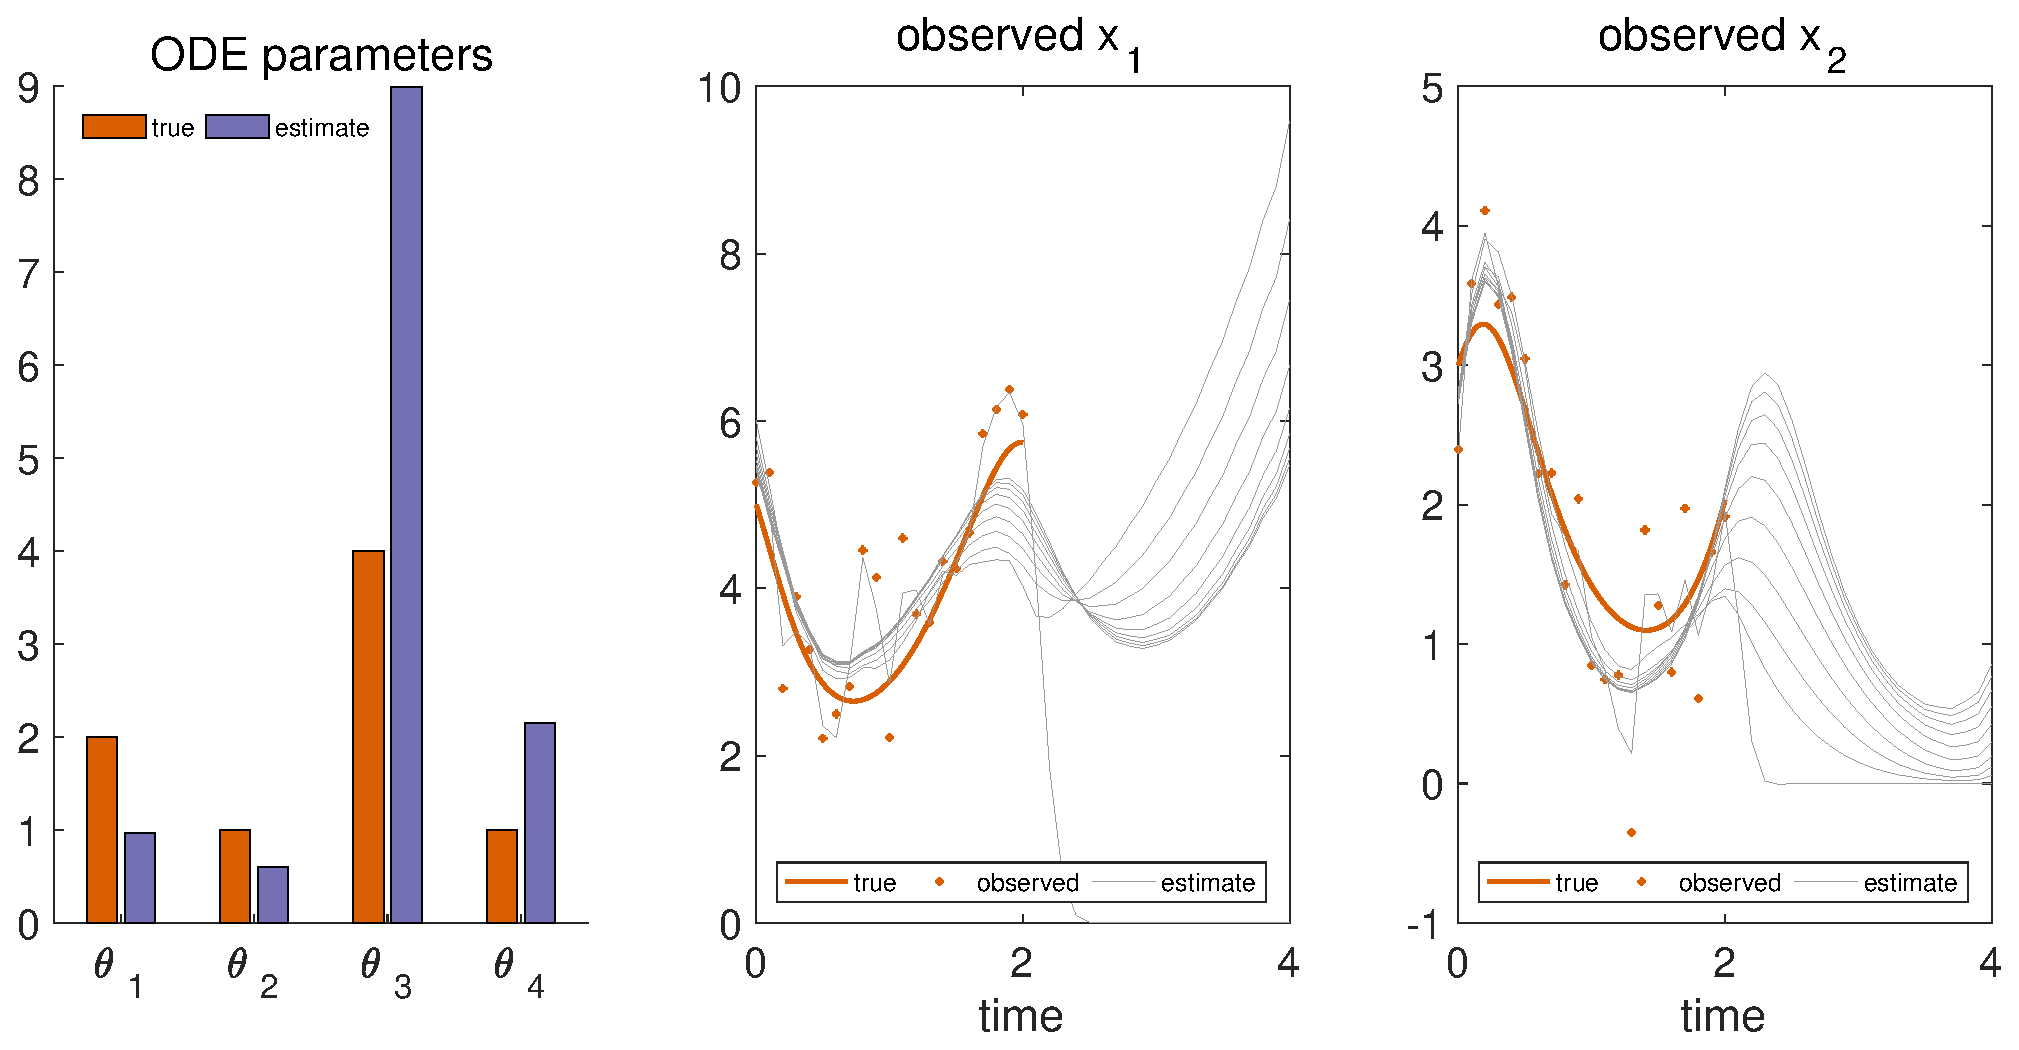
\includegraphics [width=5in]{VGM_for_Lotka_Volterra_11.eps}

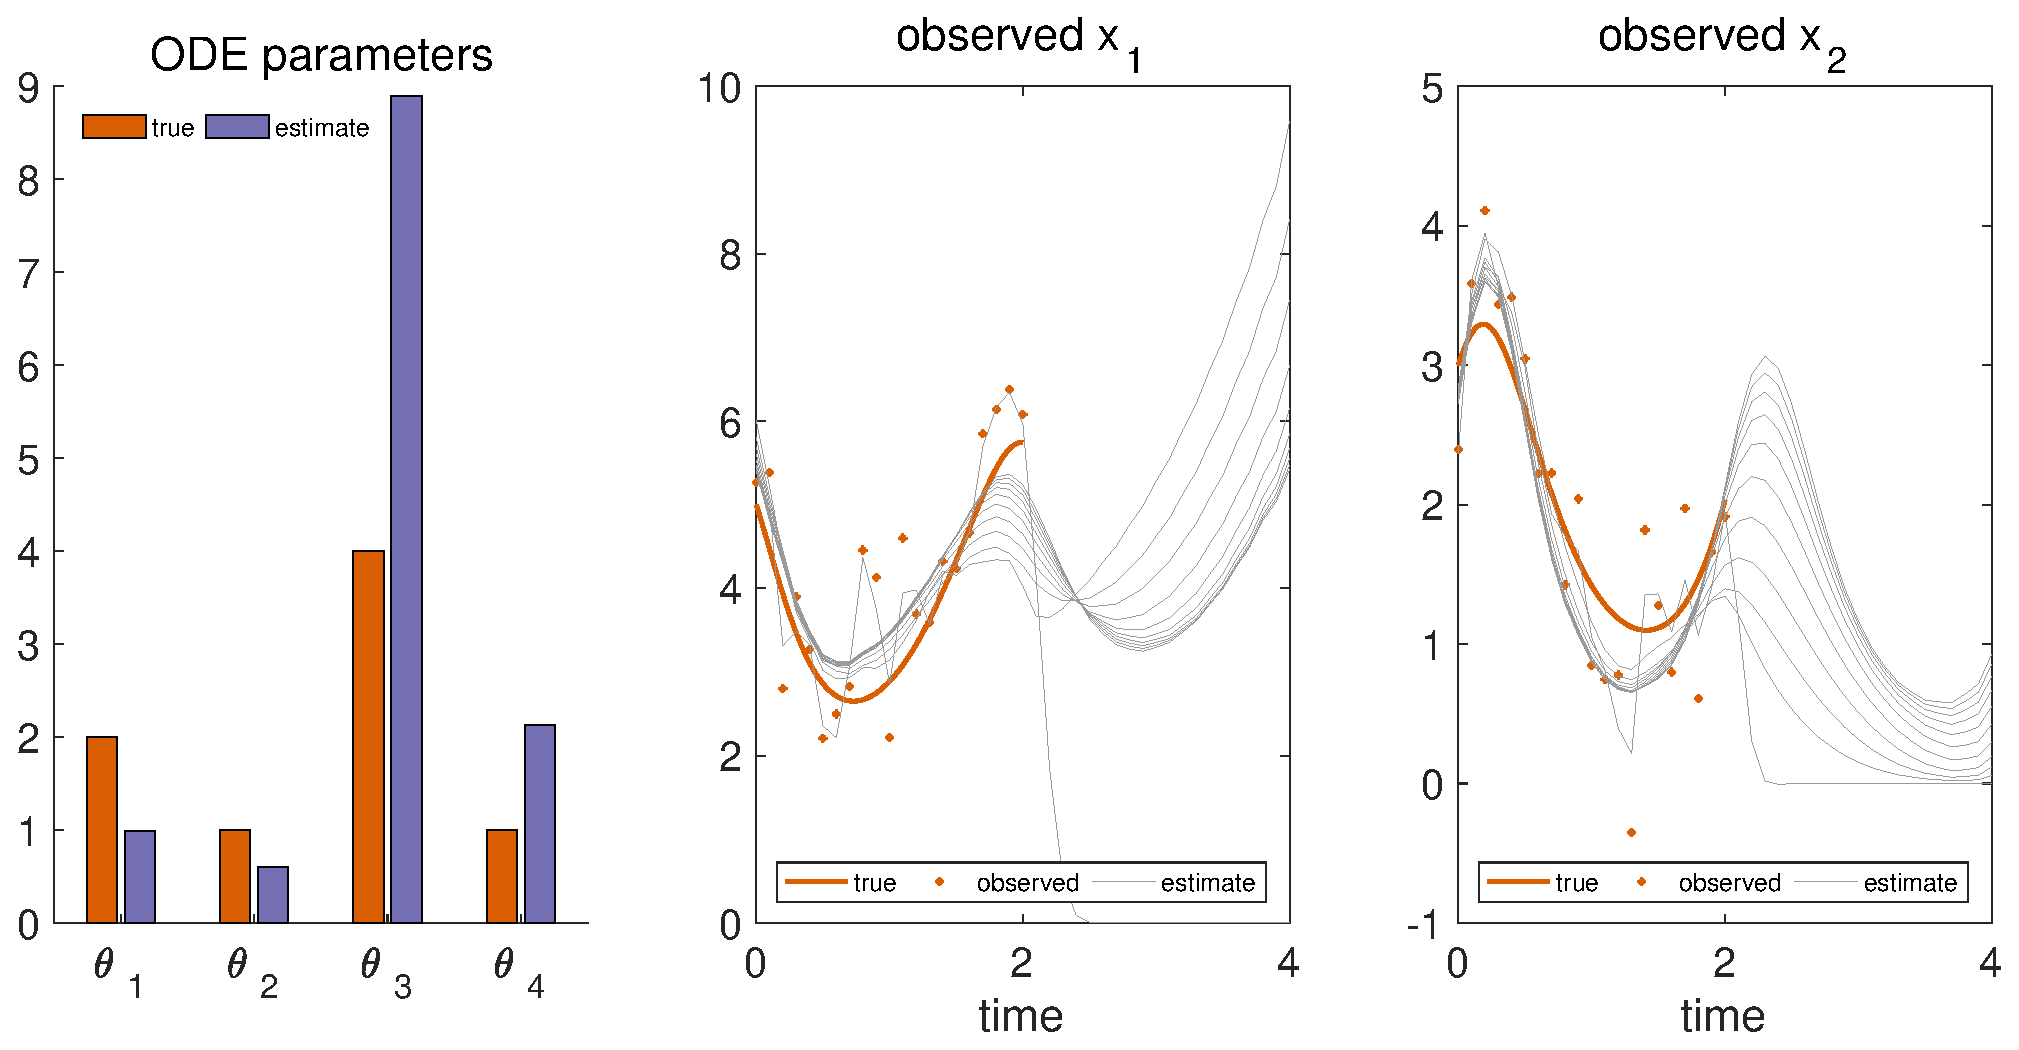
\includegraphics [width=5in]{VGM_for_Lotka_Volterra_12.eps}

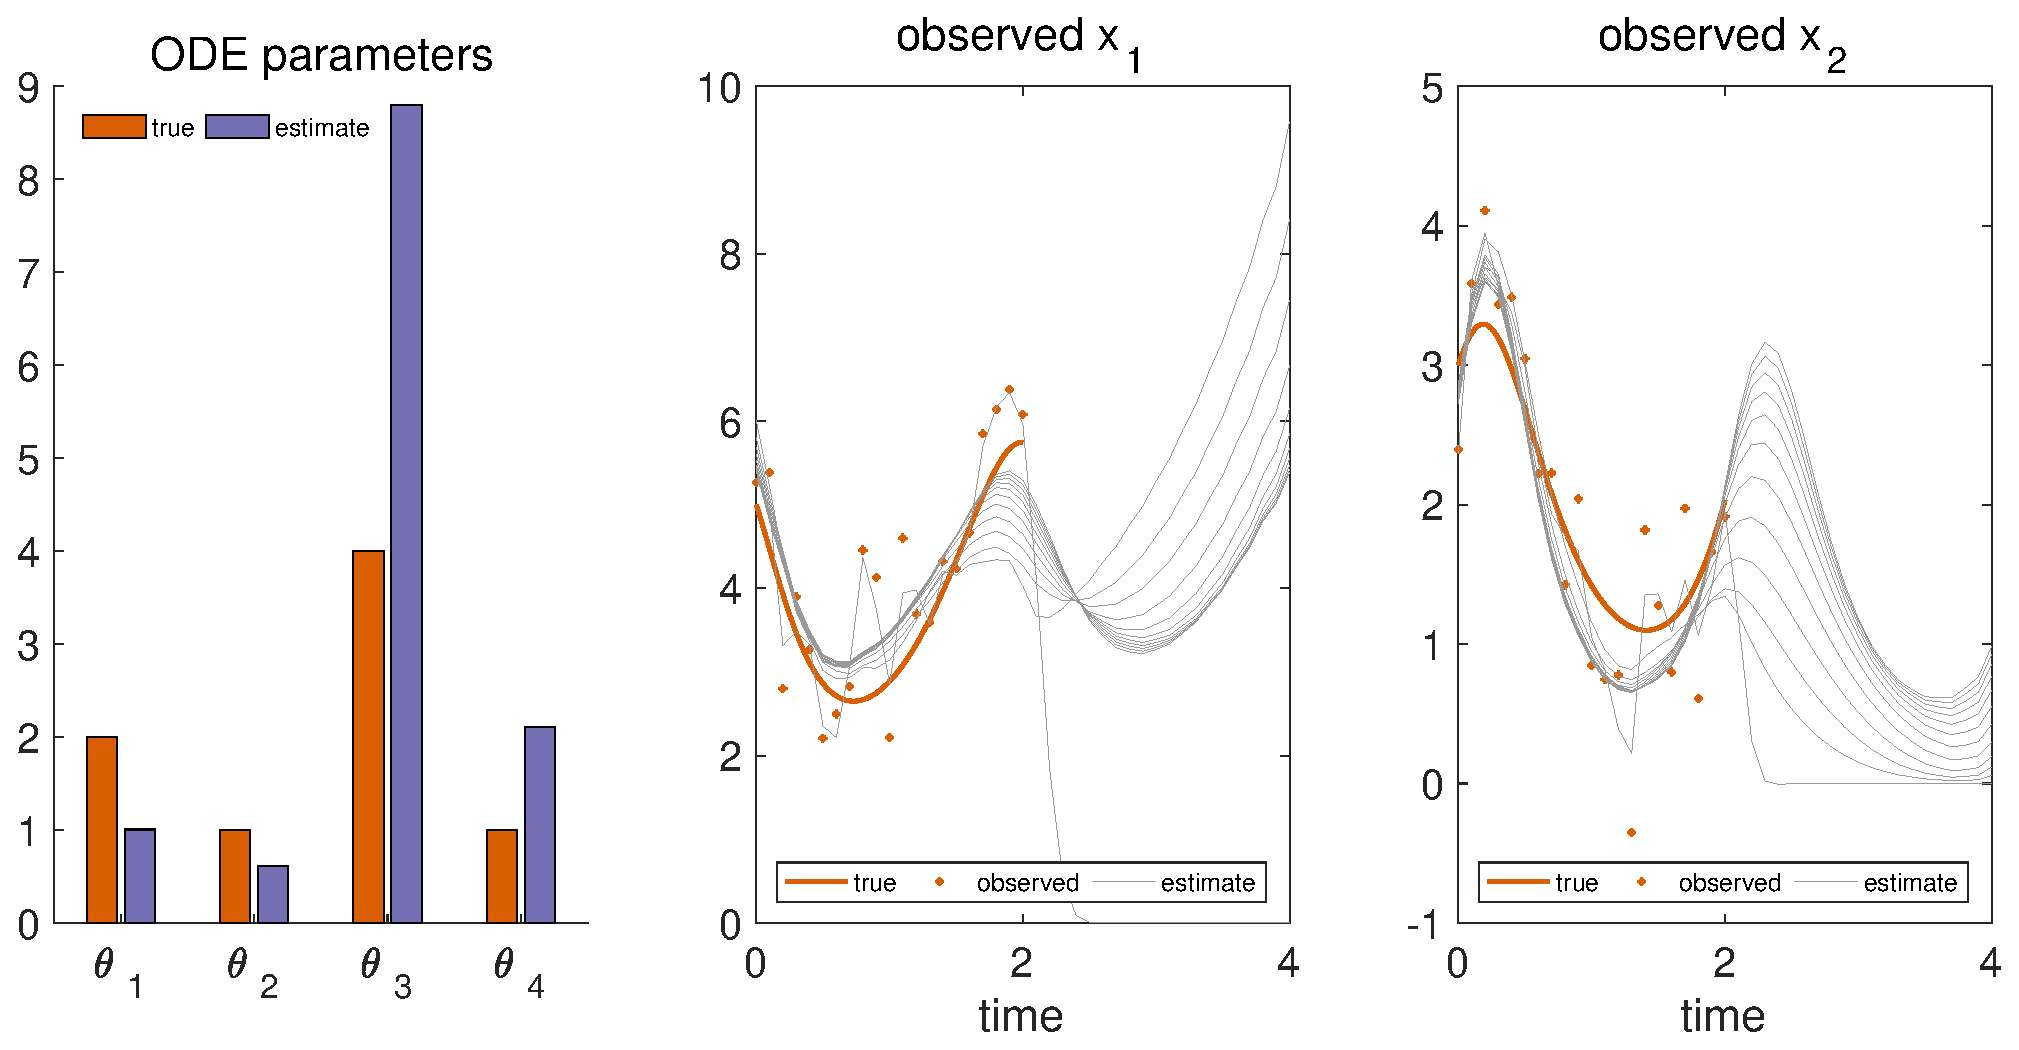
\includegraphics [width=5in]{VGM_for_Lotka_Volterra_13.eps}

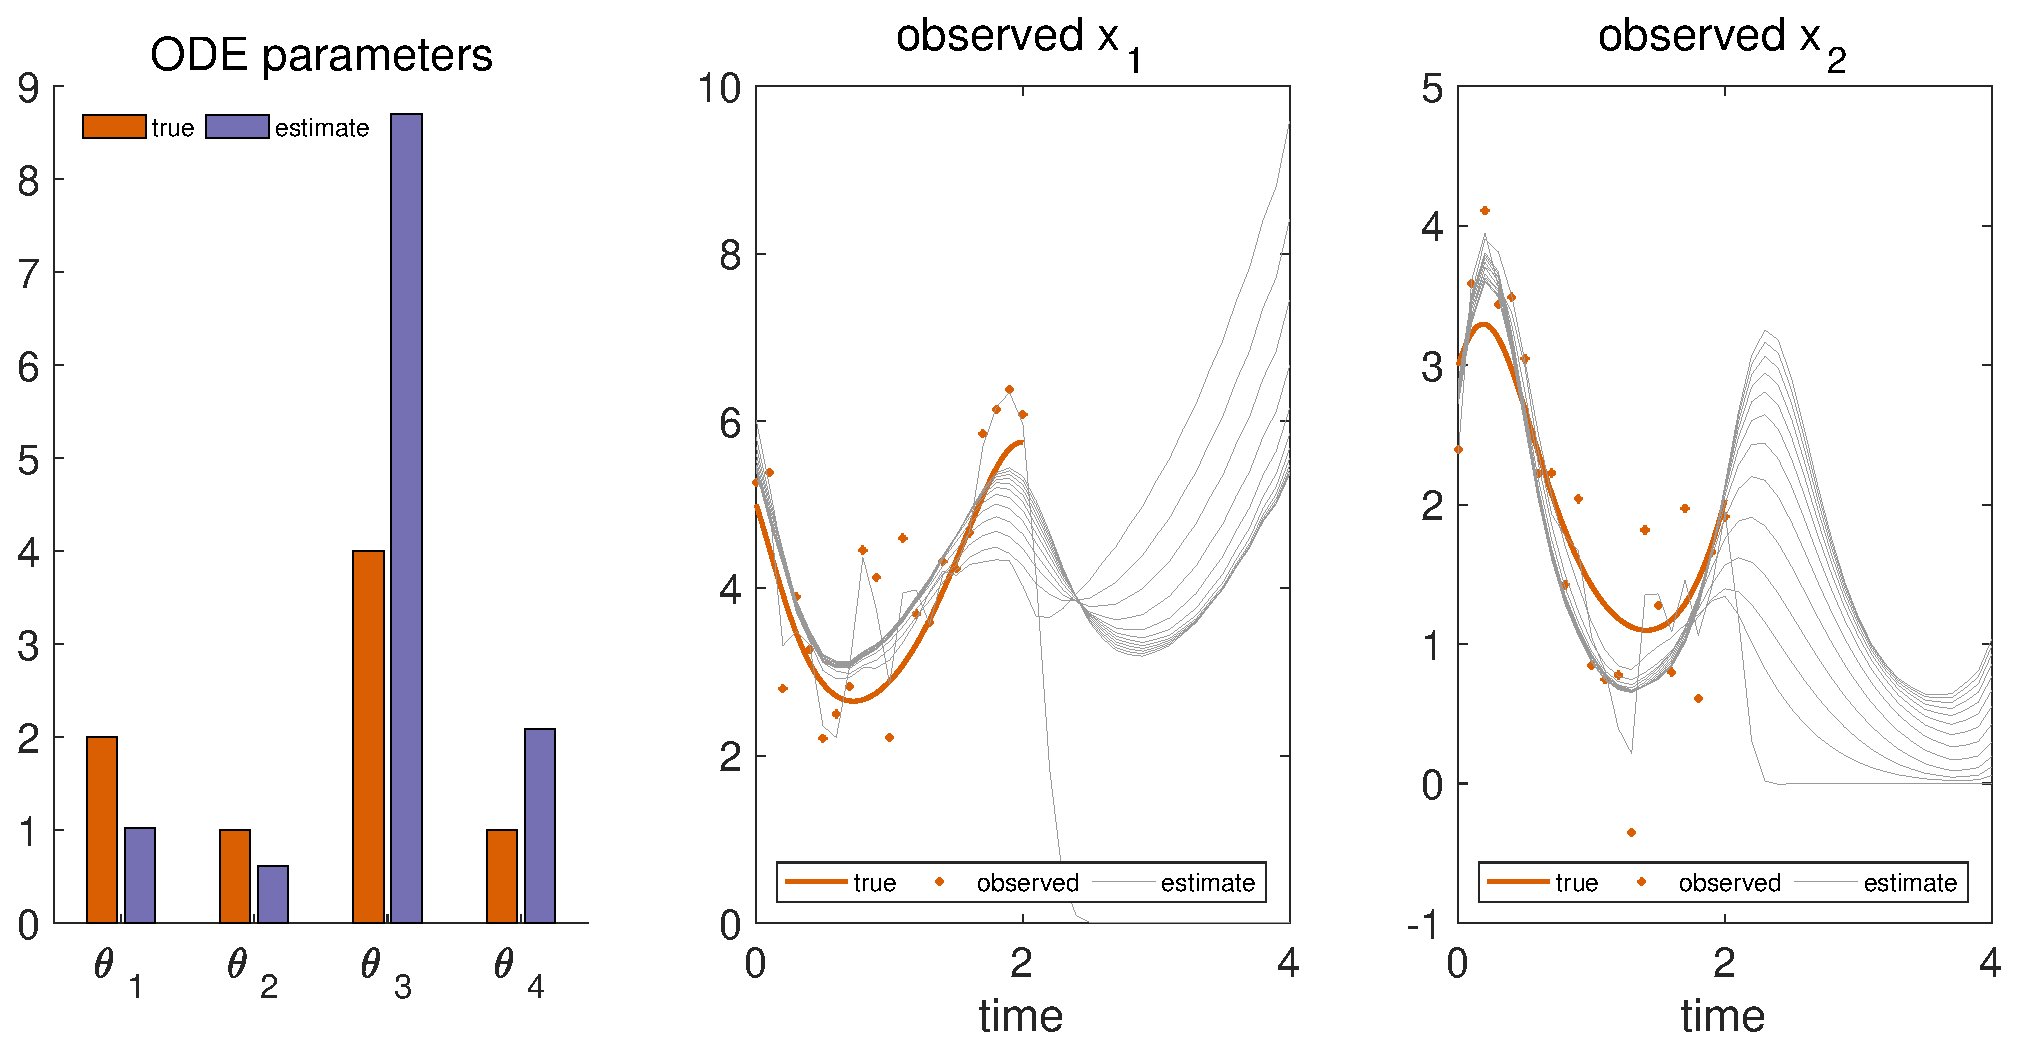
\includegraphics [width=5in]{VGM_for_Lotka_Volterra_14.eps}

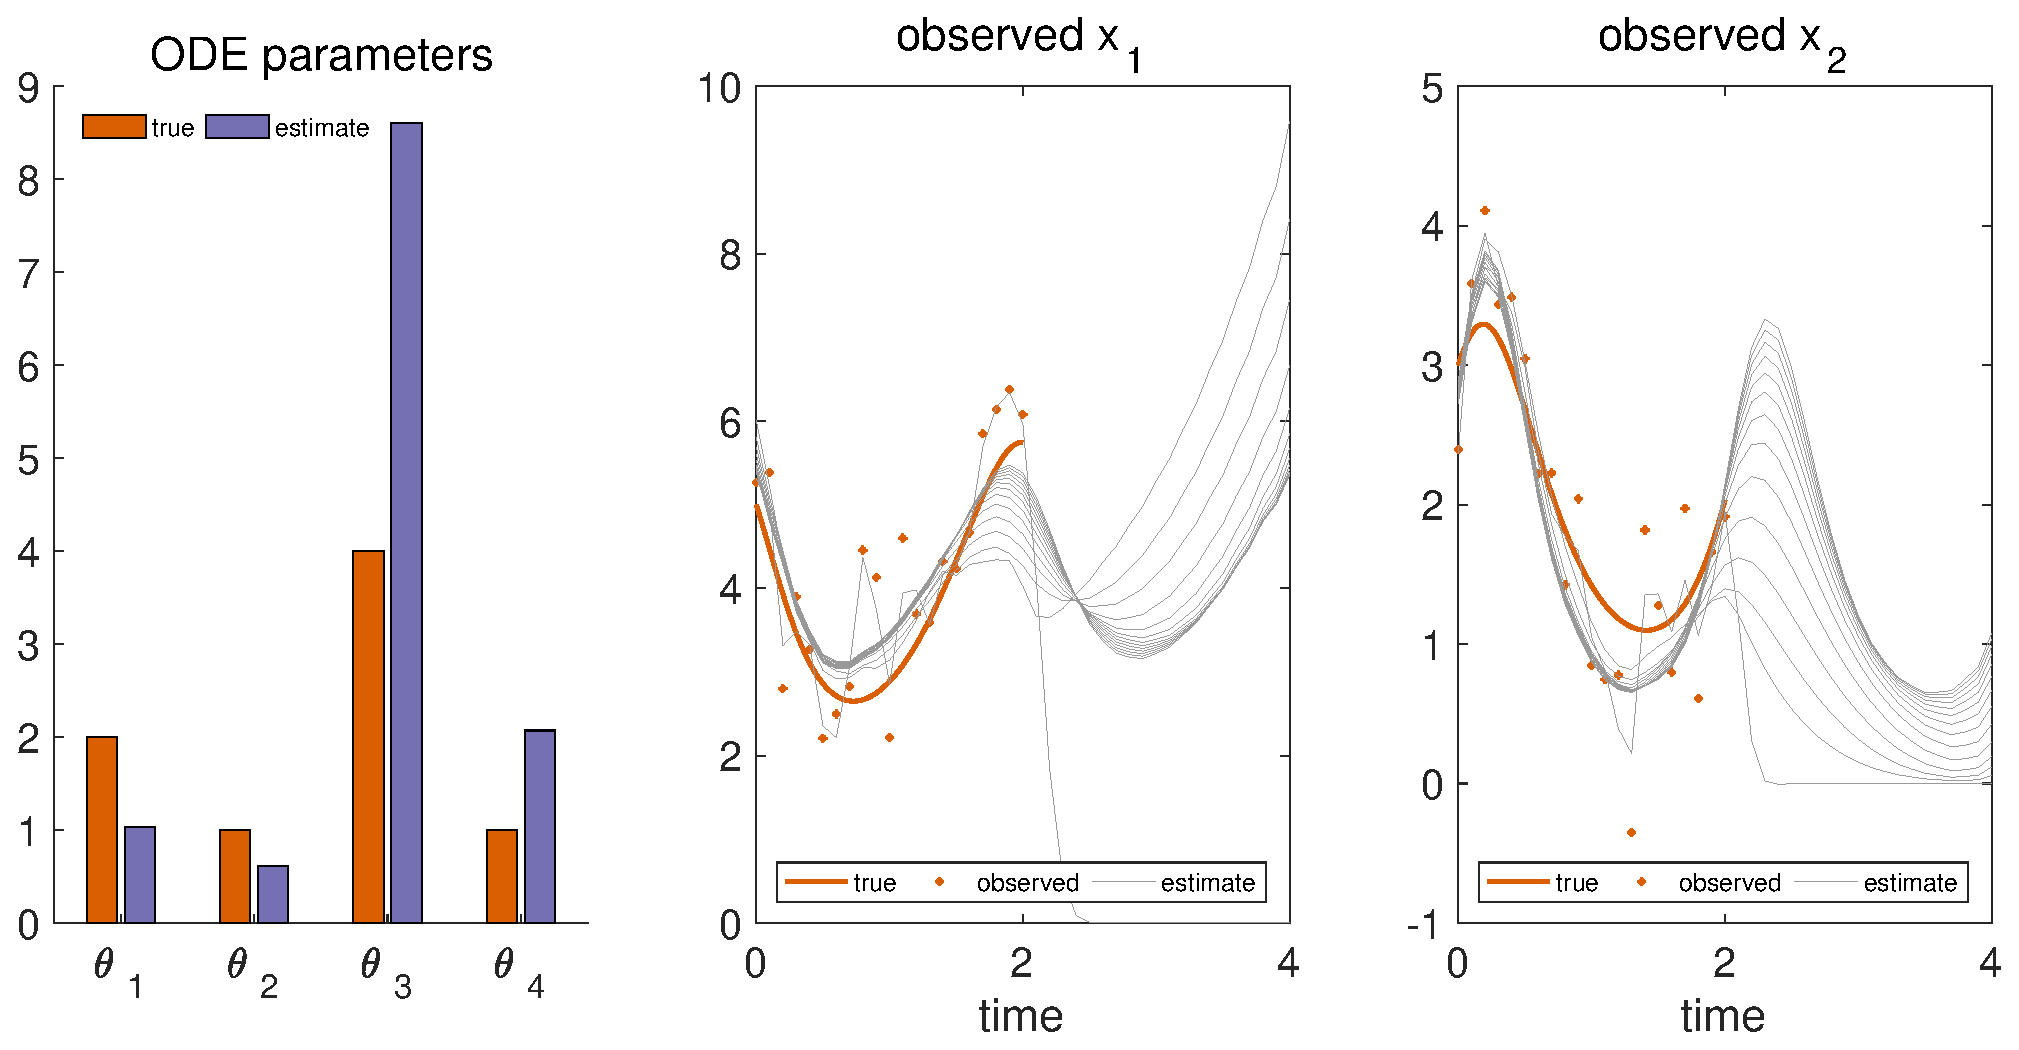
\includegraphics [width=5in]{VGM_for_Lotka_Volterra_15.eps}

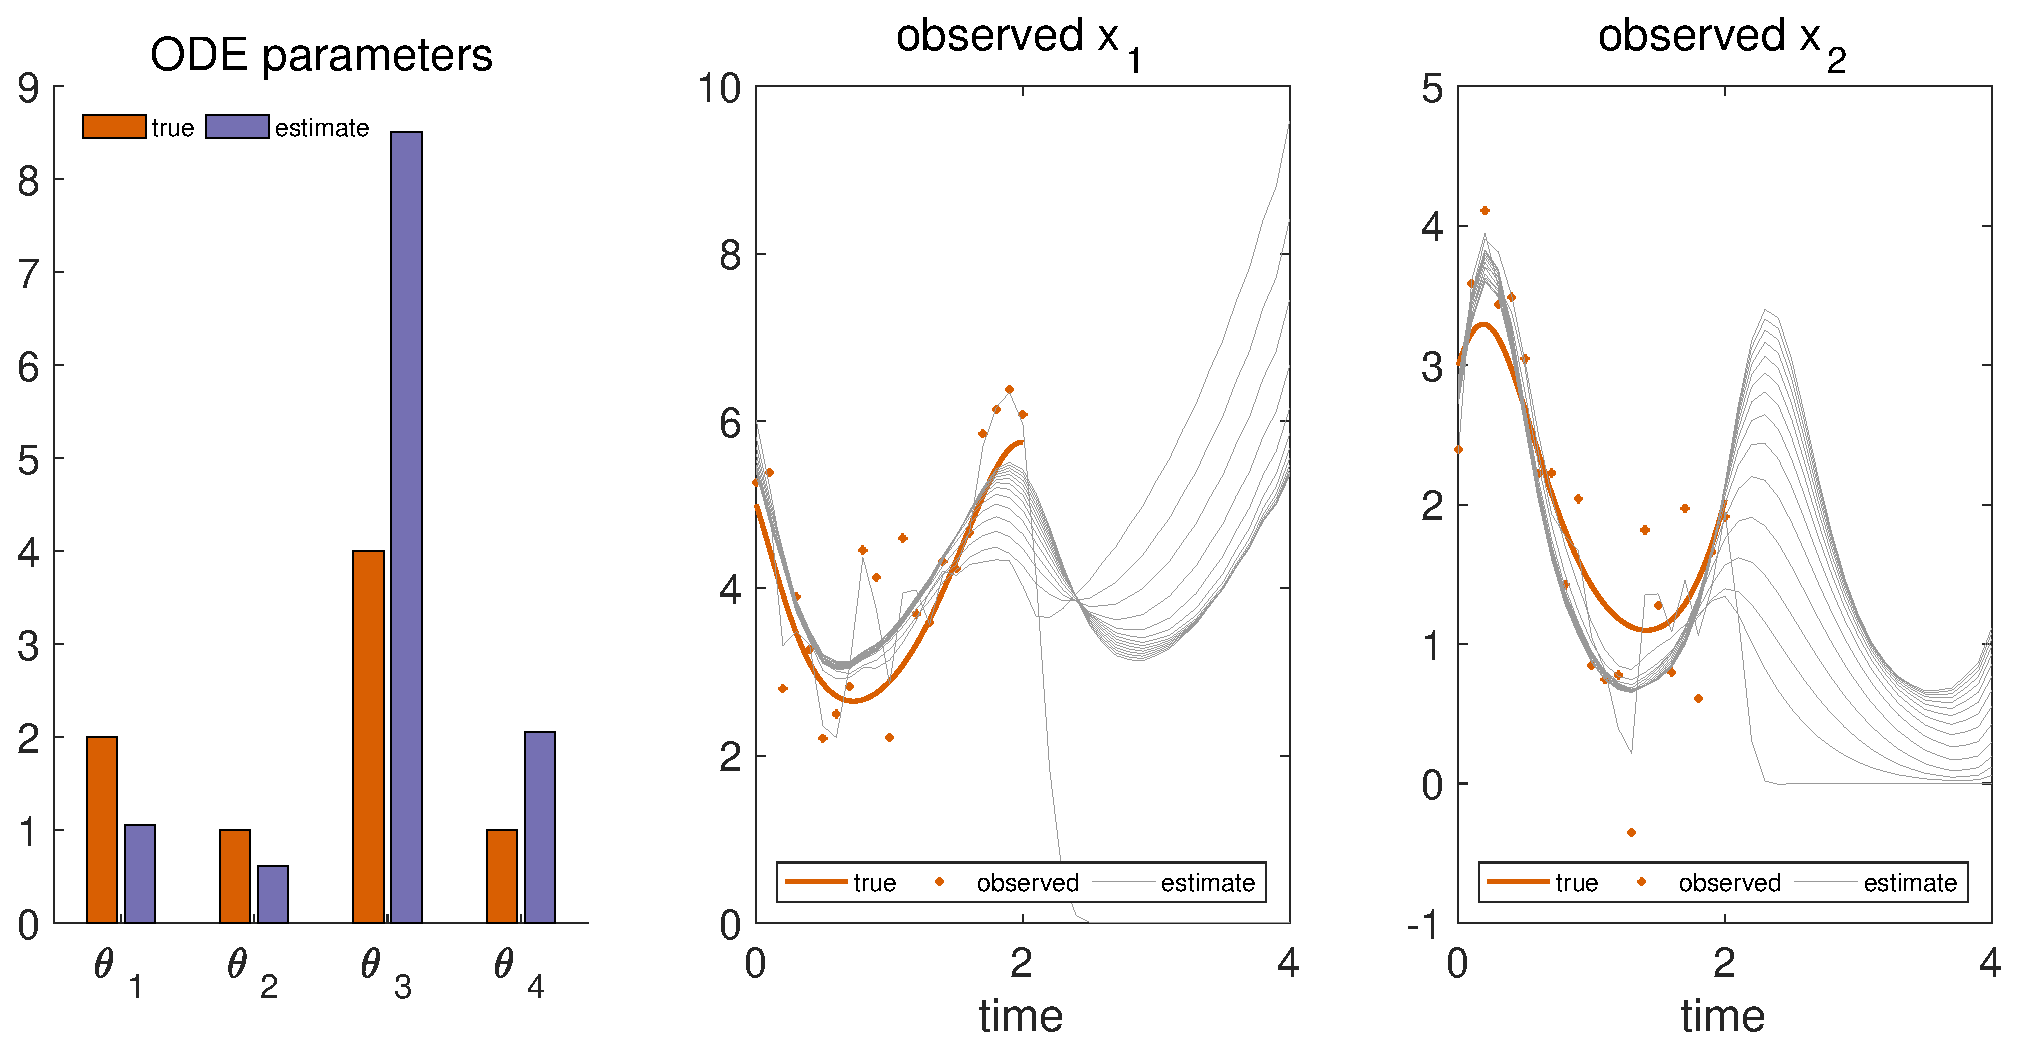
\includegraphics [width=5in]{VGM_for_Lotka_Volterra_16.eps}

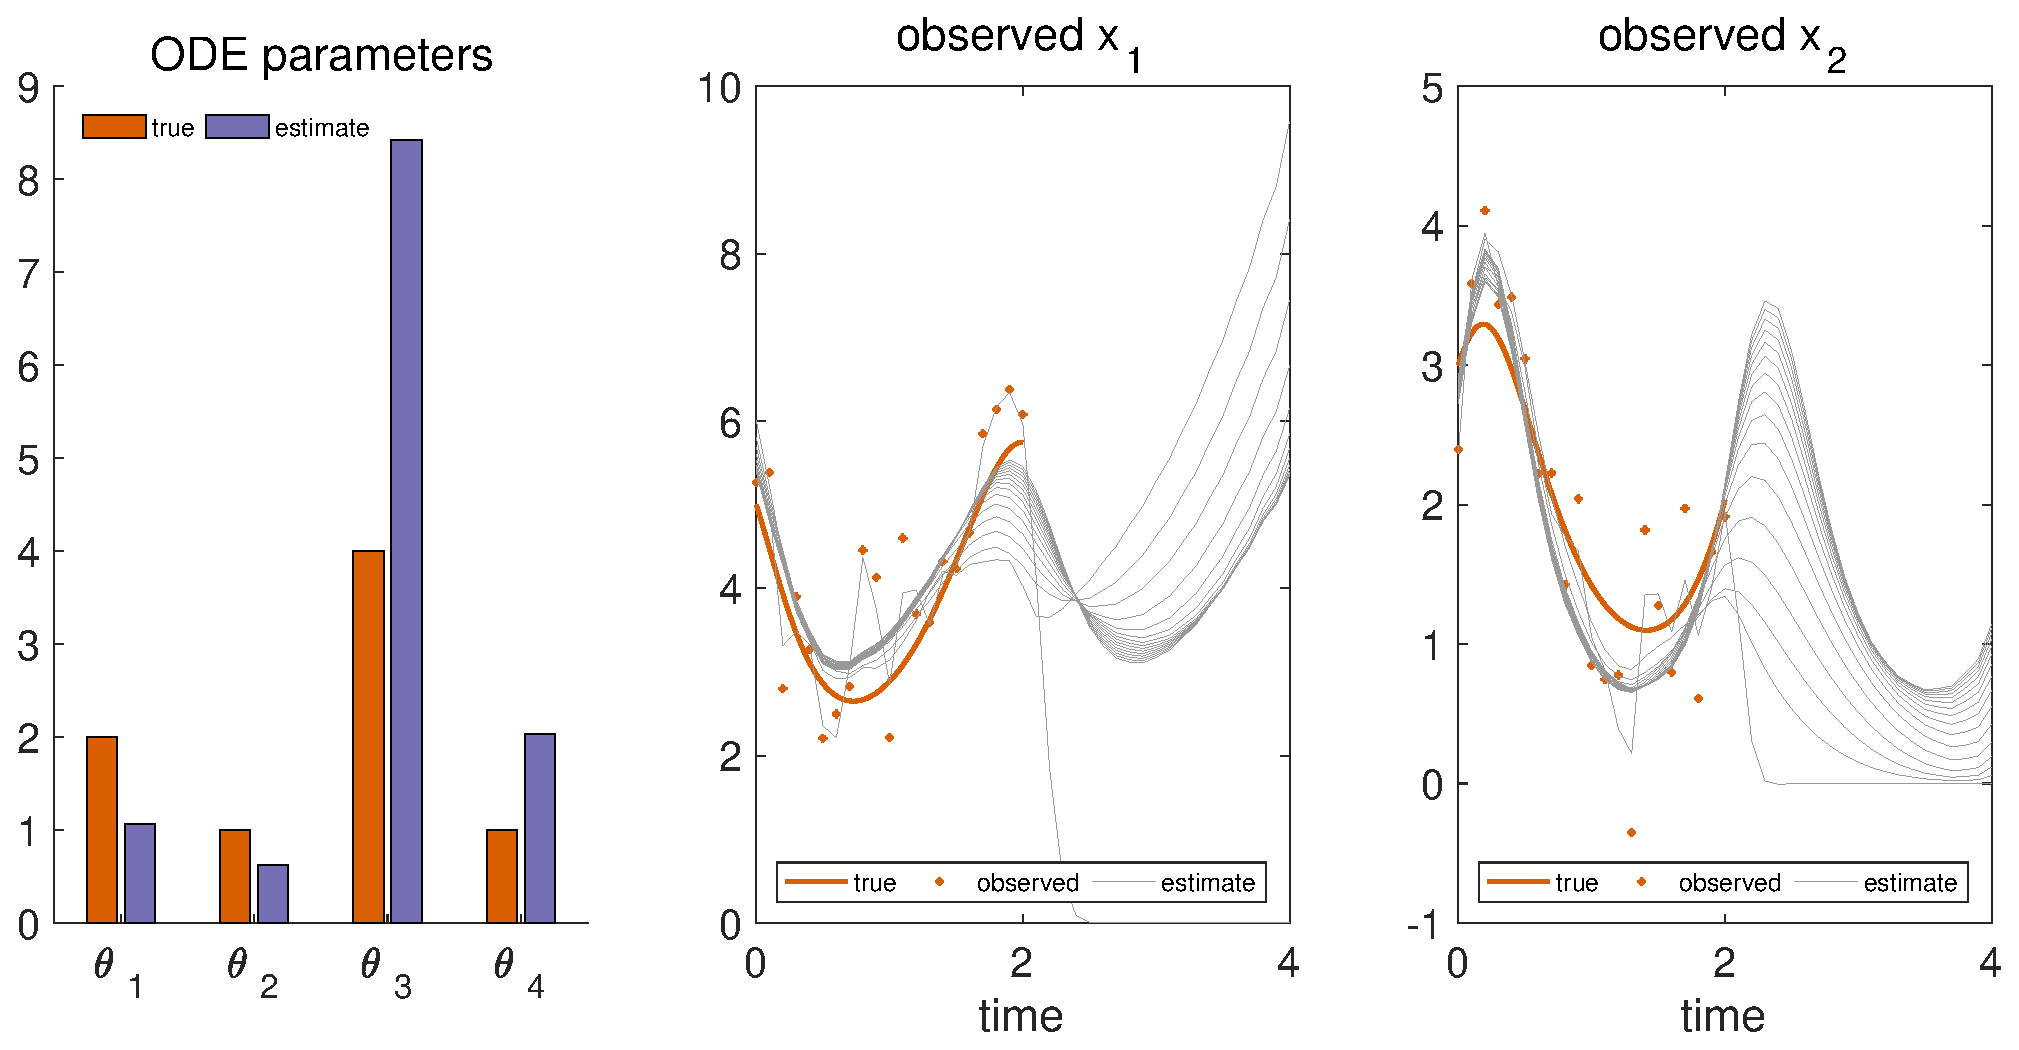
\includegraphics [width=5in]{VGM_for_Lotka_Volterra_17.eps}

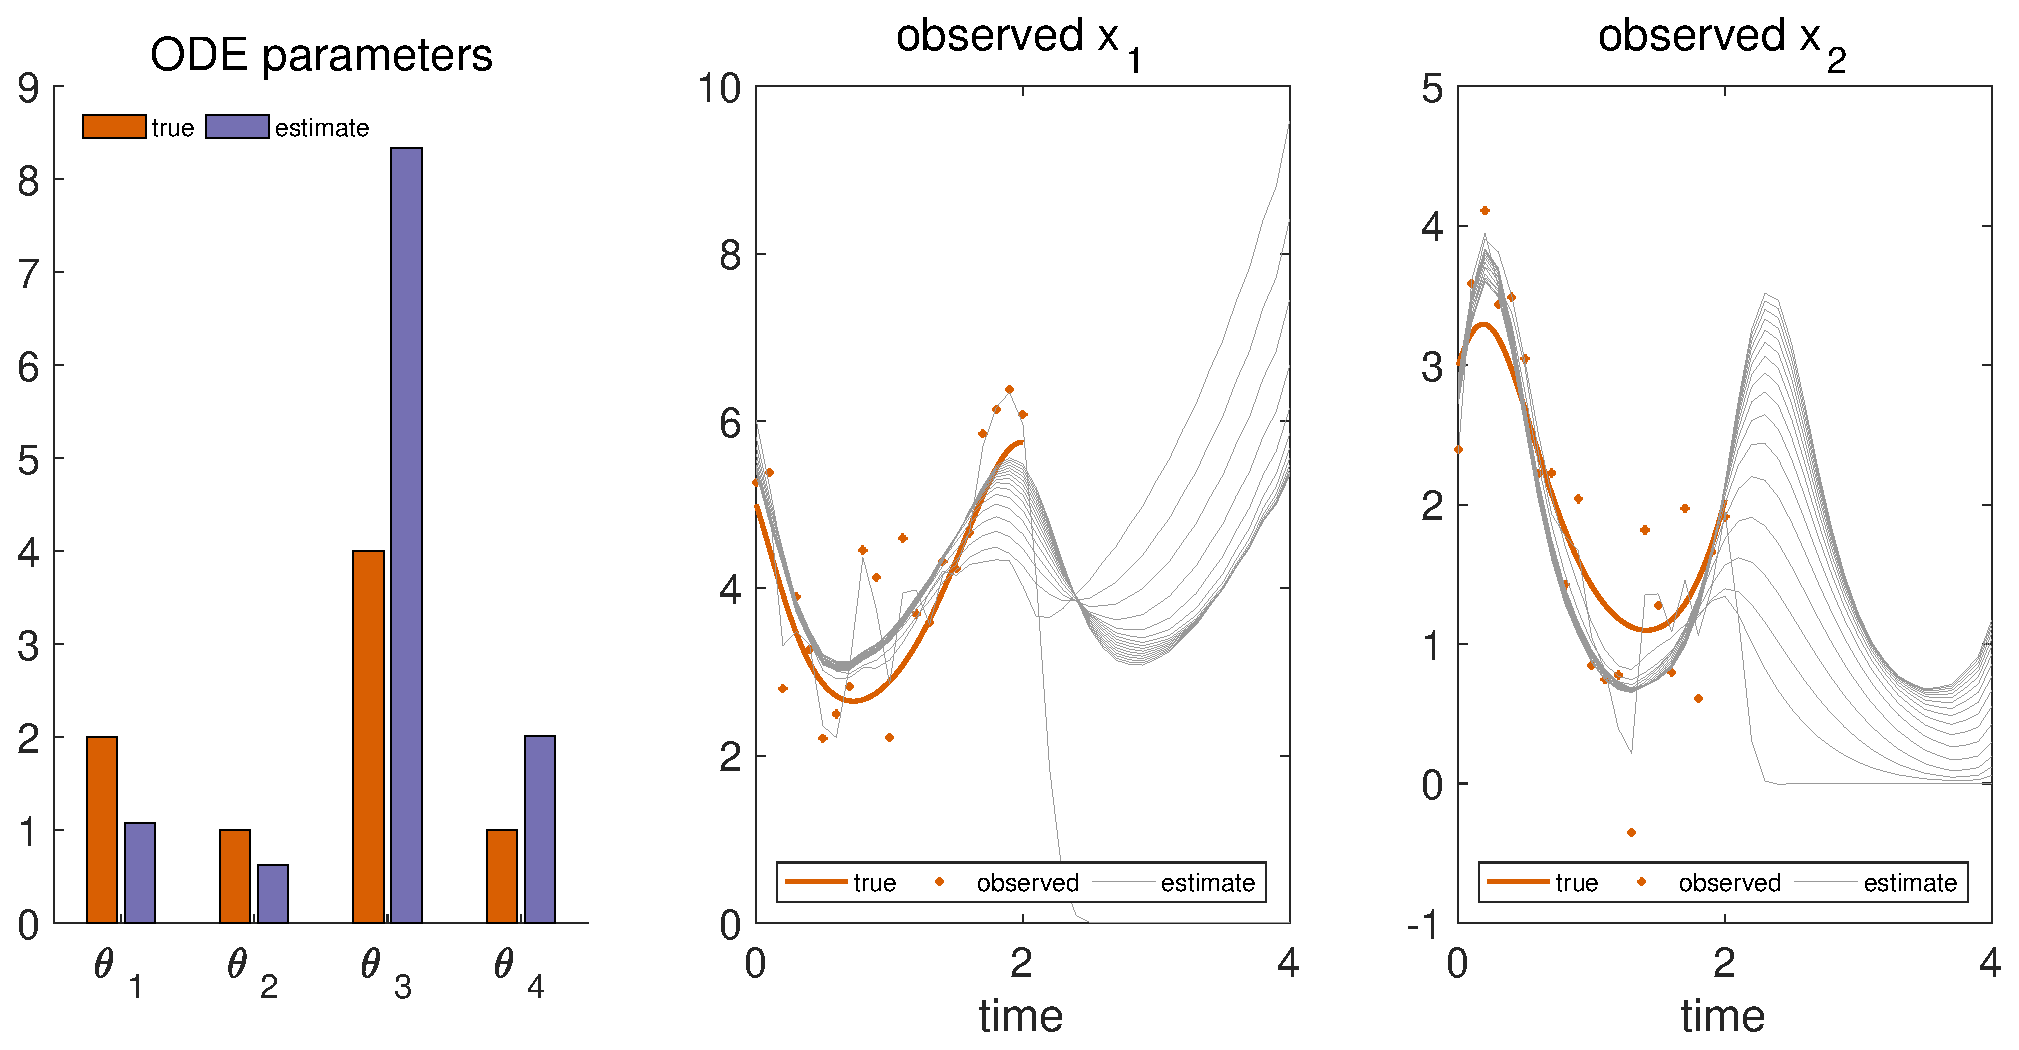
\includegraphics [width=5in]{VGM_for_Lotka_Volterra_18.eps}

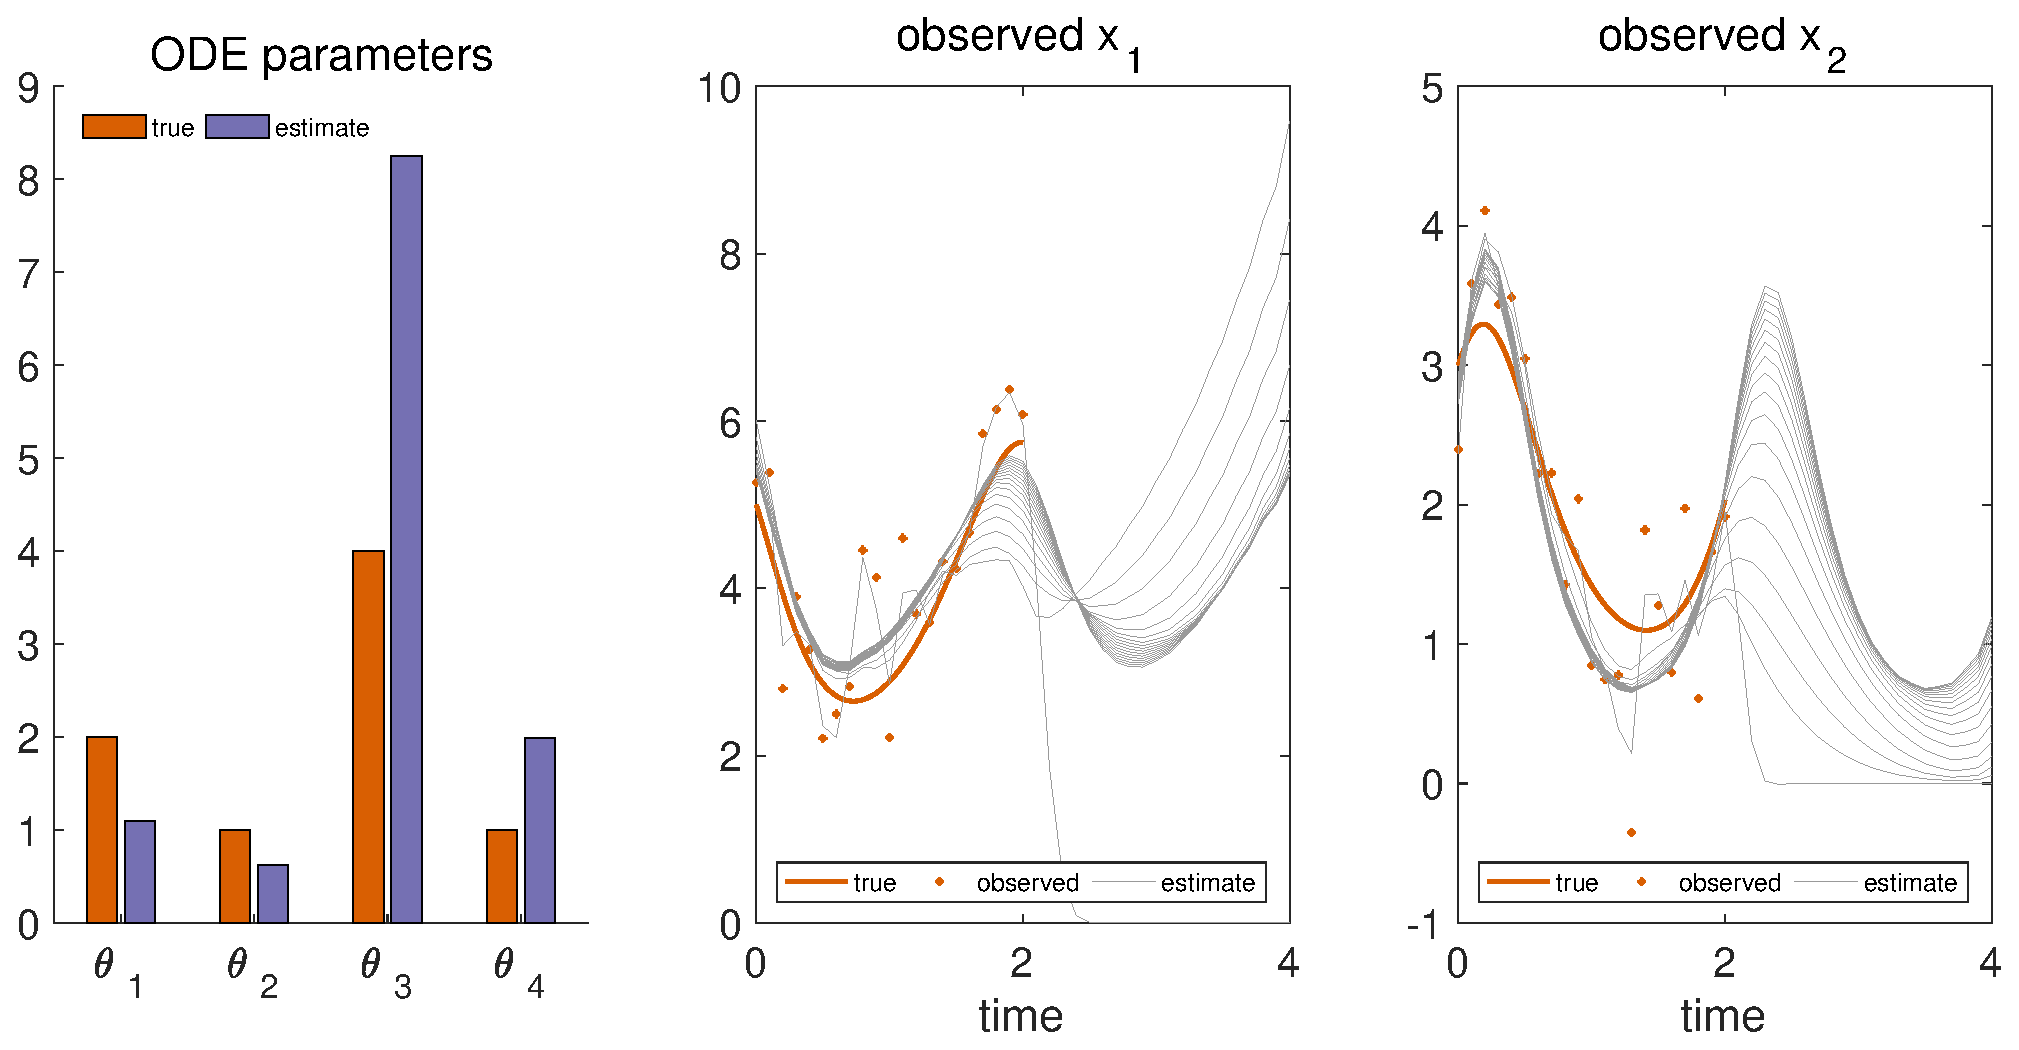
\includegraphics [width=5in]{VGM_for_Lotka_Volterra_19.eps}

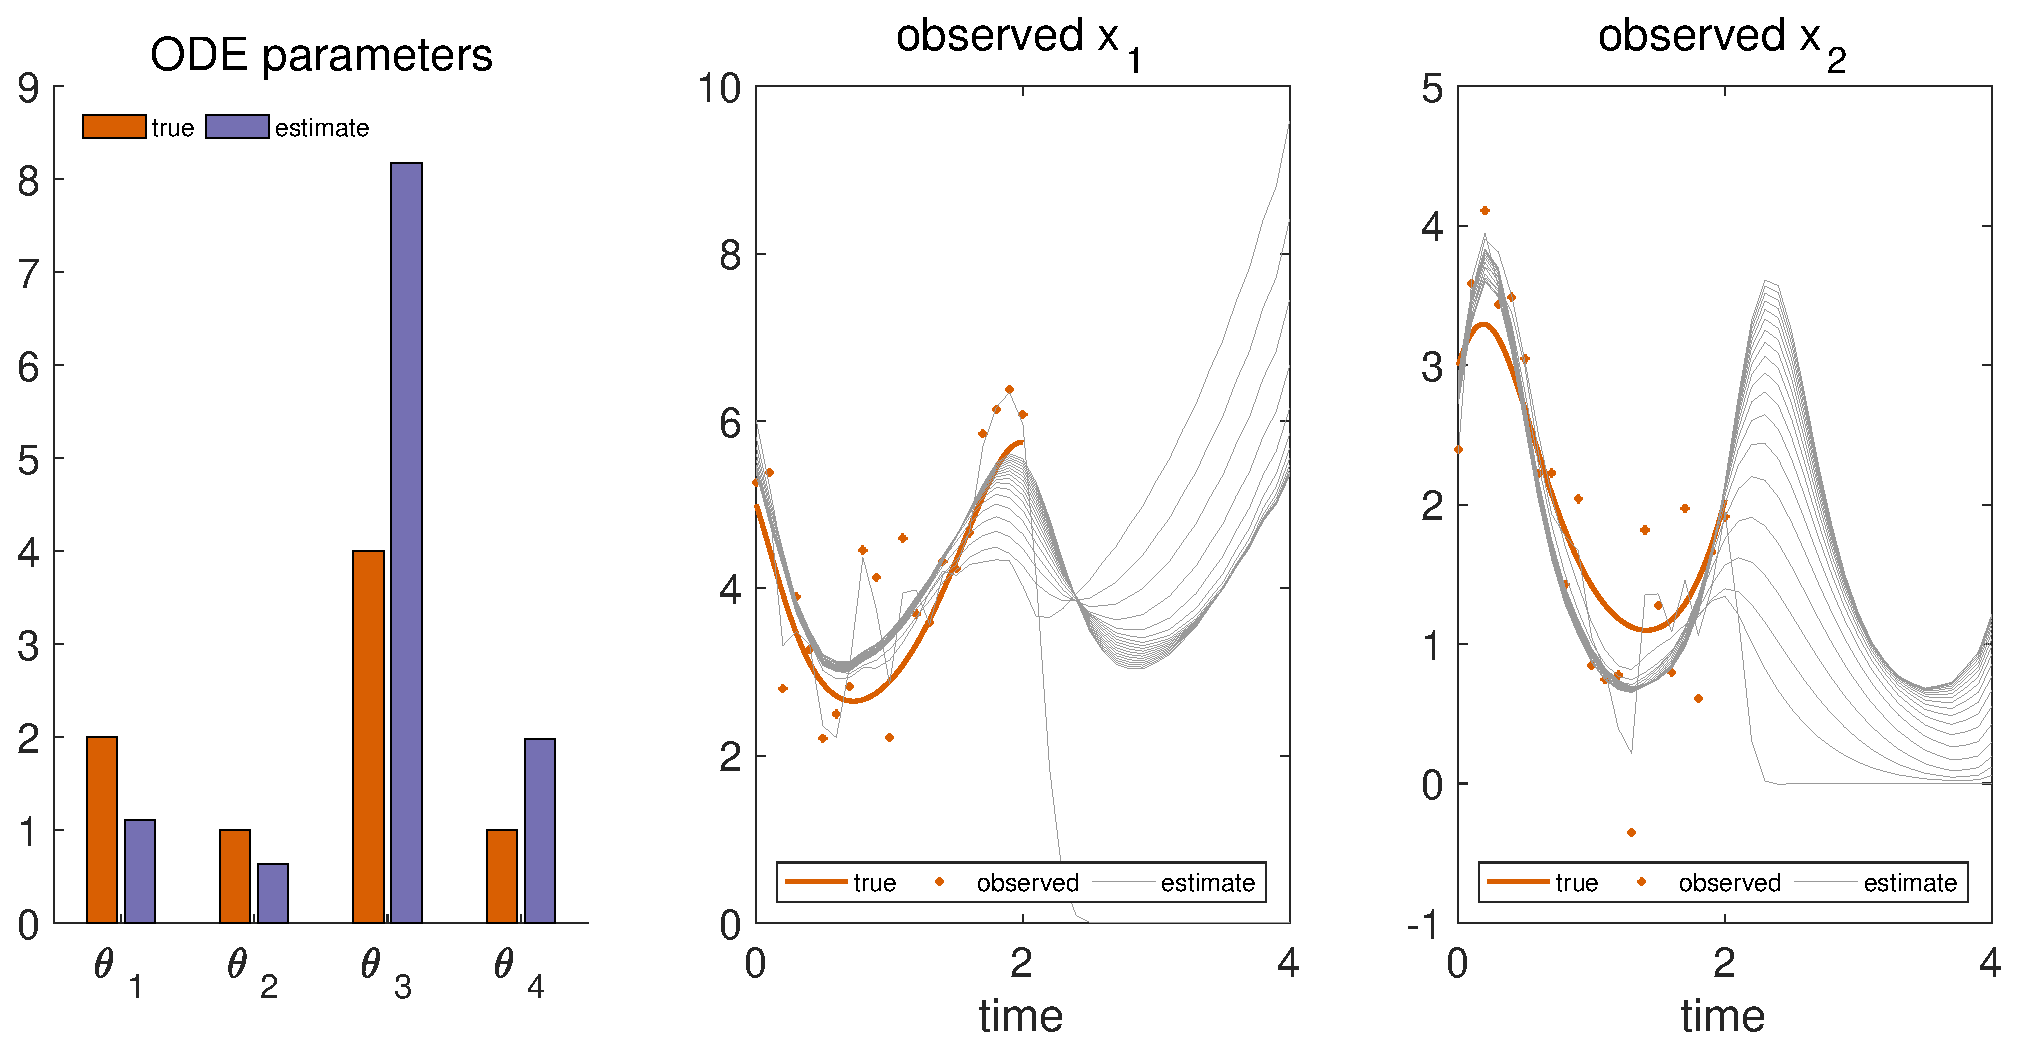
\includegraphics [width=5in]{VGM_for_Lotka_Volterra_20.eps}

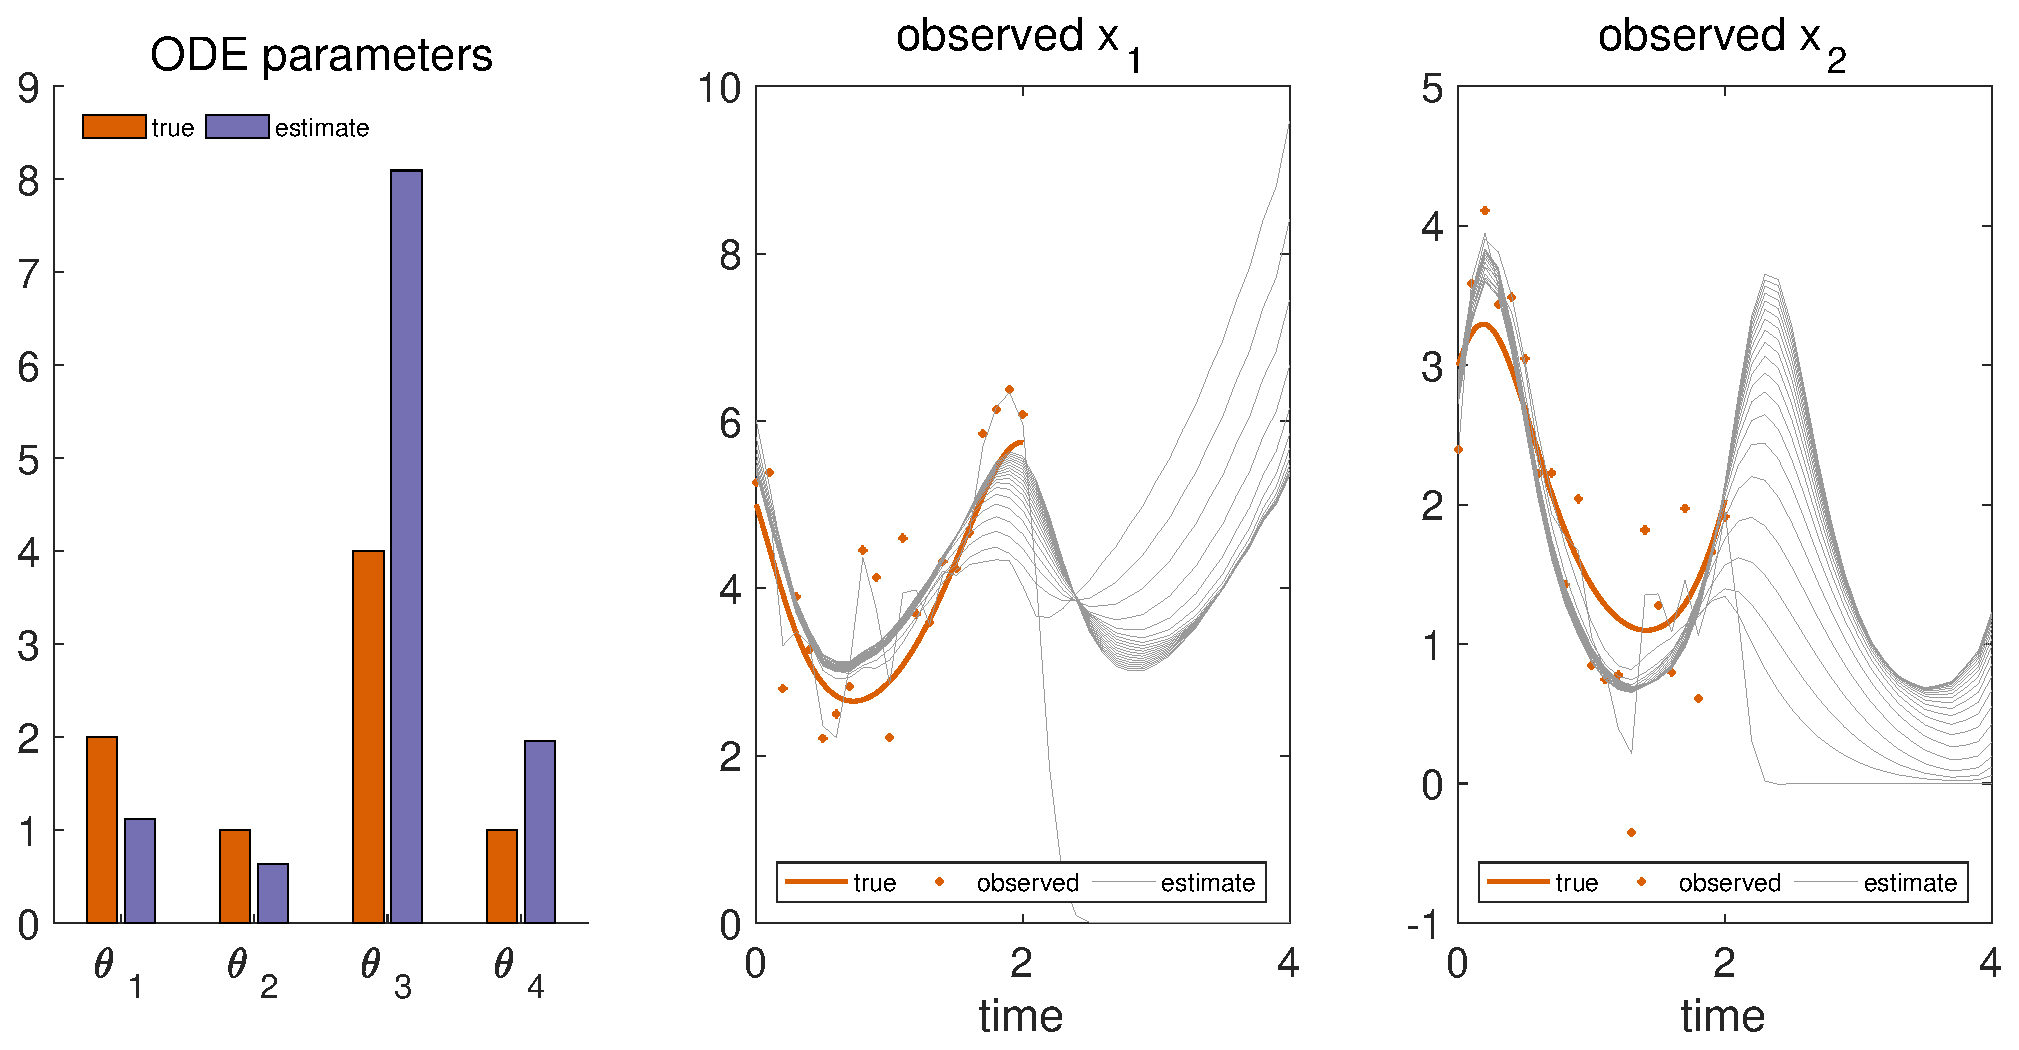
\includegraphics [width=5in]{VGM_for_Lotka_Volterra_21.eps}

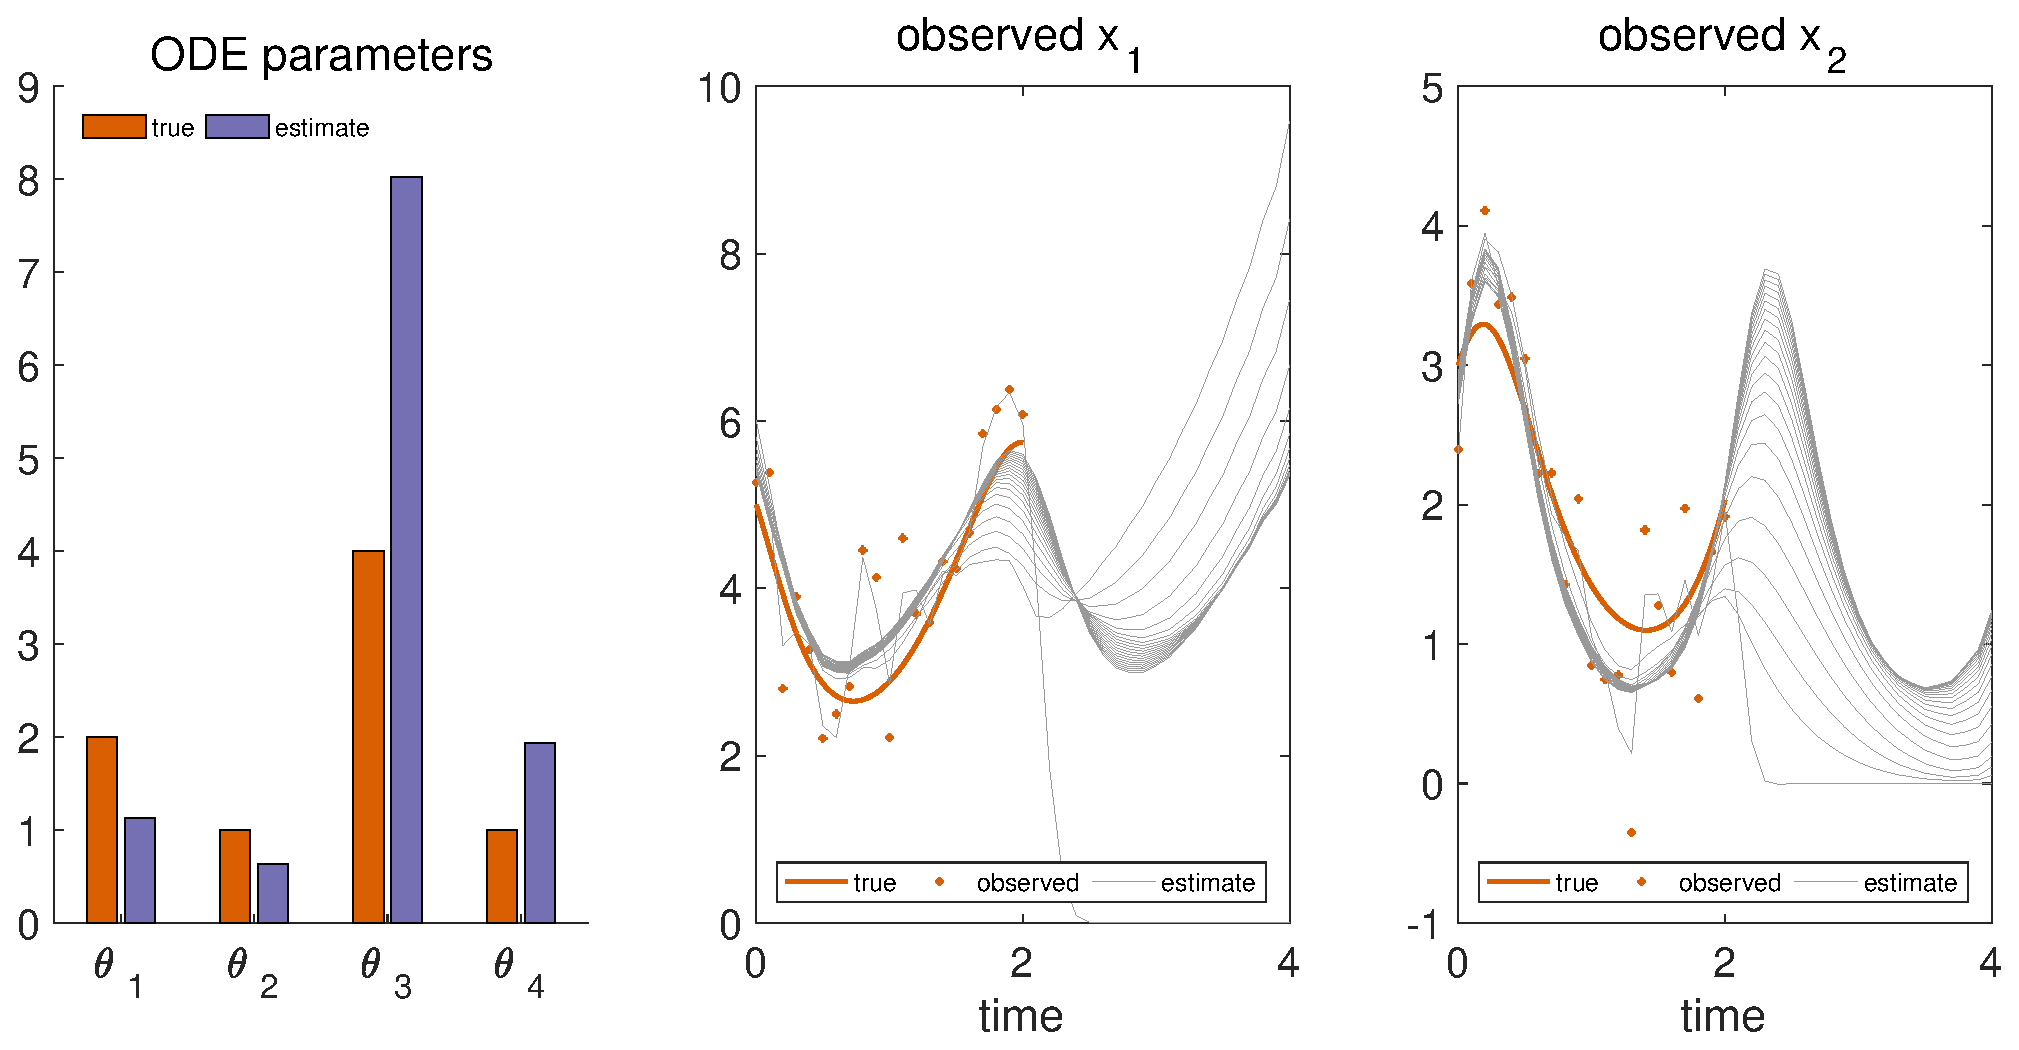
\includegraphics [width=5in]{VGM_for_Lotka_Volterra_22.eps}

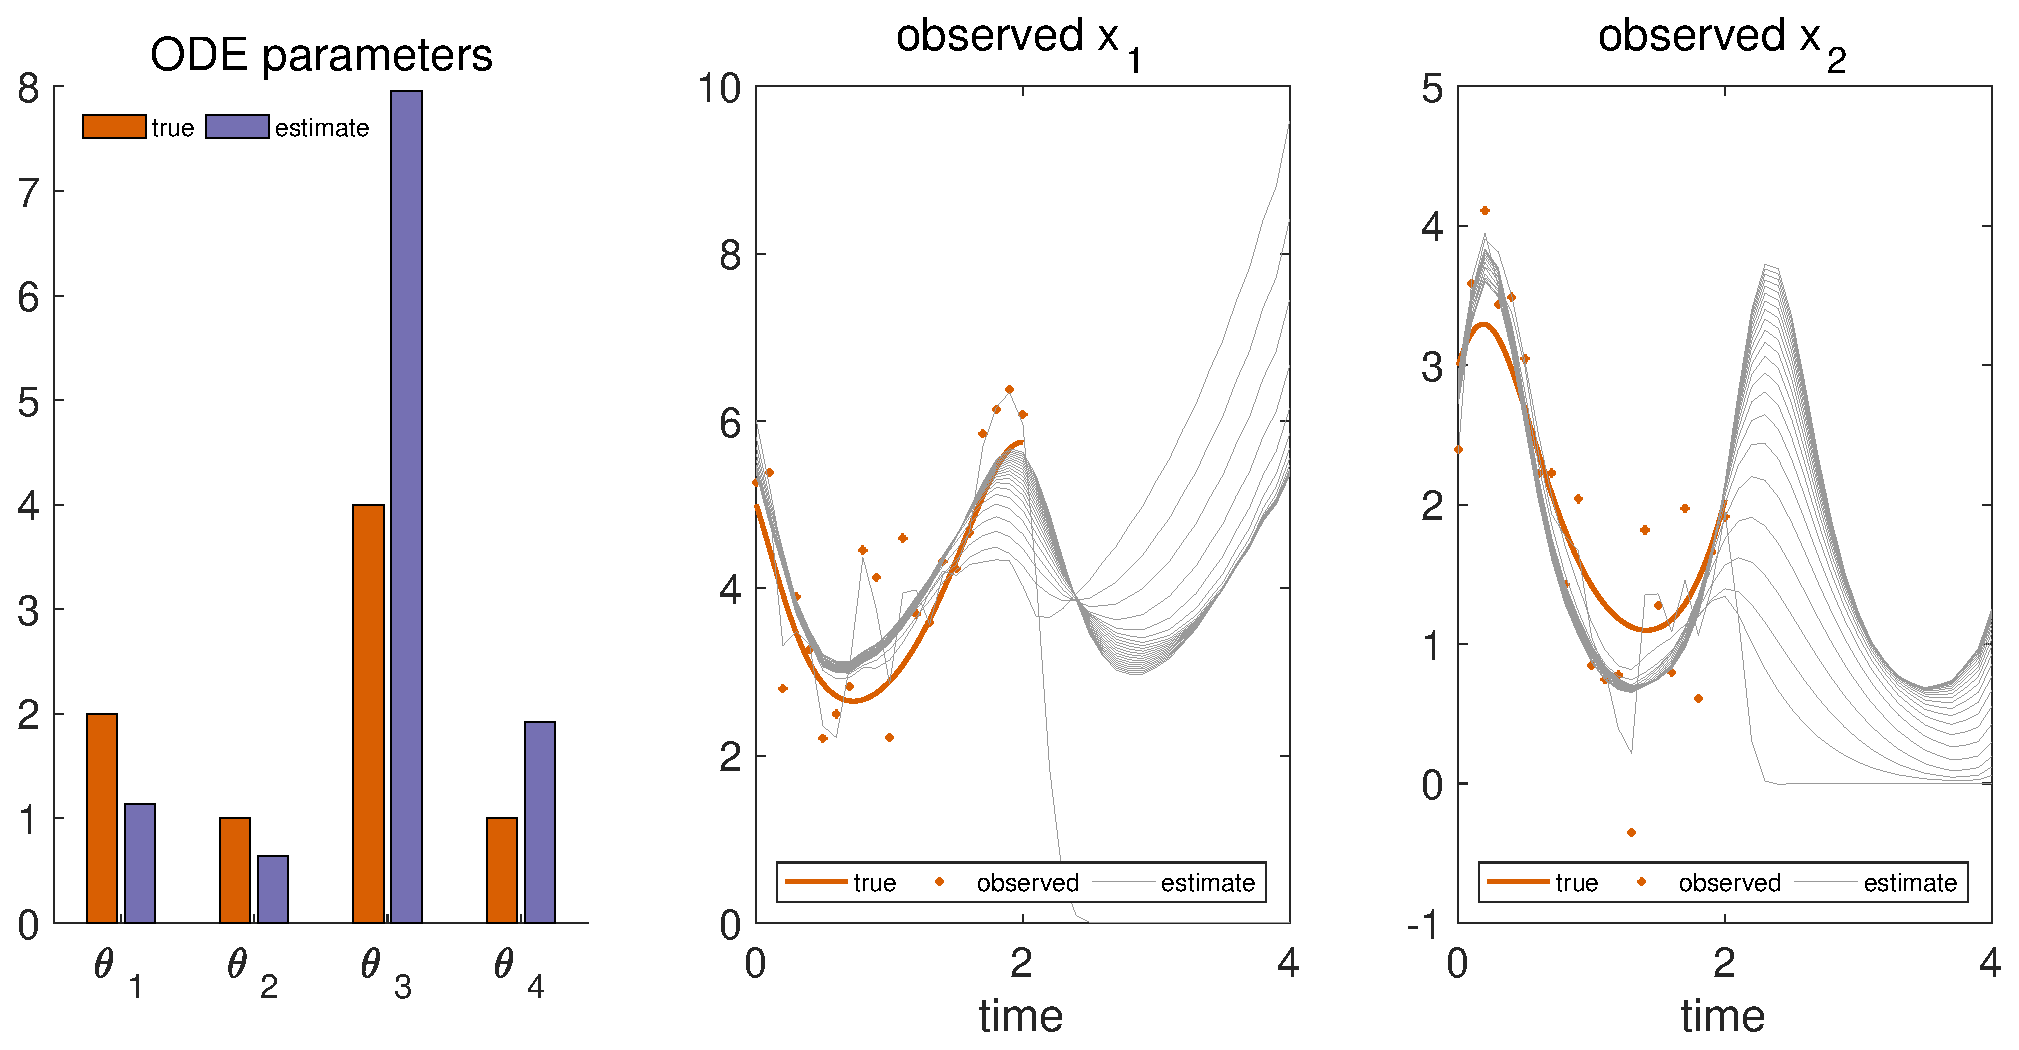
\includegraphics [width=5in]{VGM_for_Lotka_Volterra_23.eps}

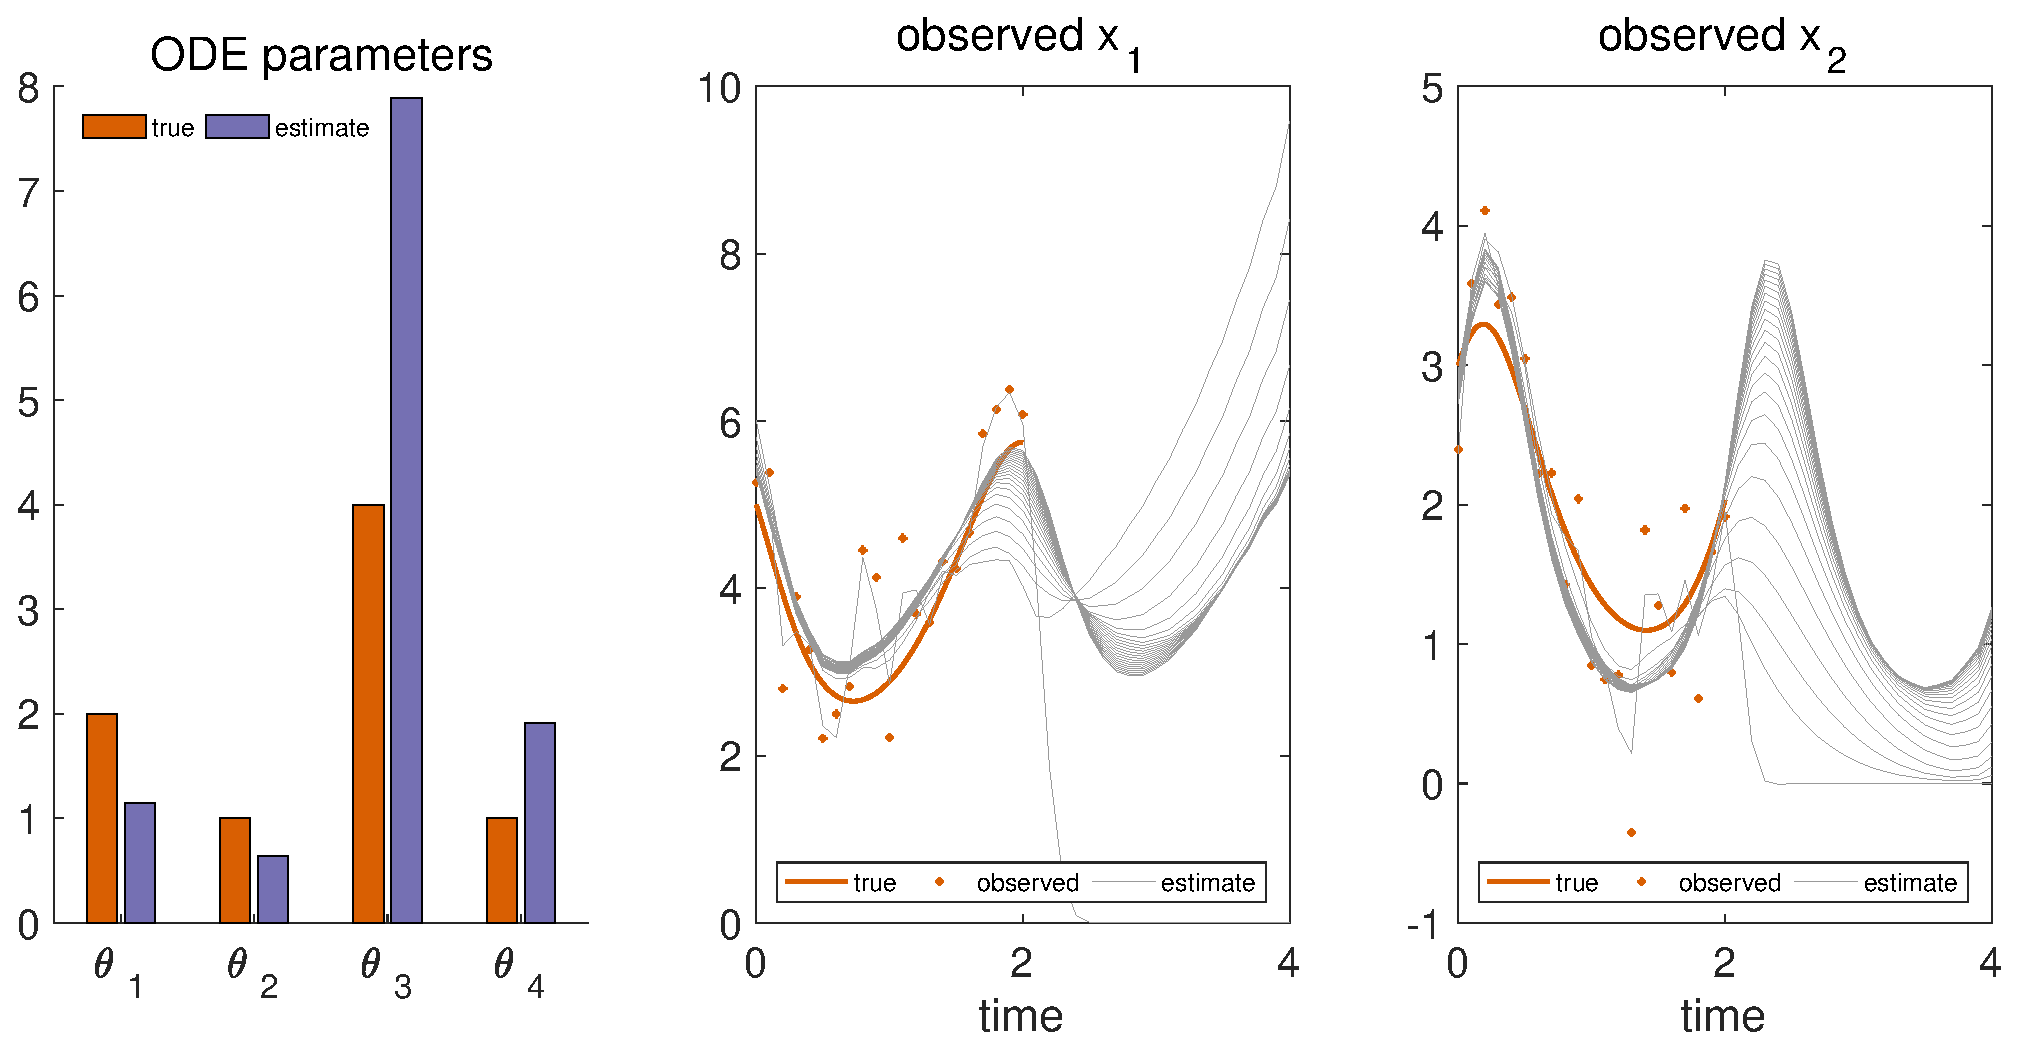
\includegraphics [width=5in]{VGM_for_Lotka_Volterra_24.eps}

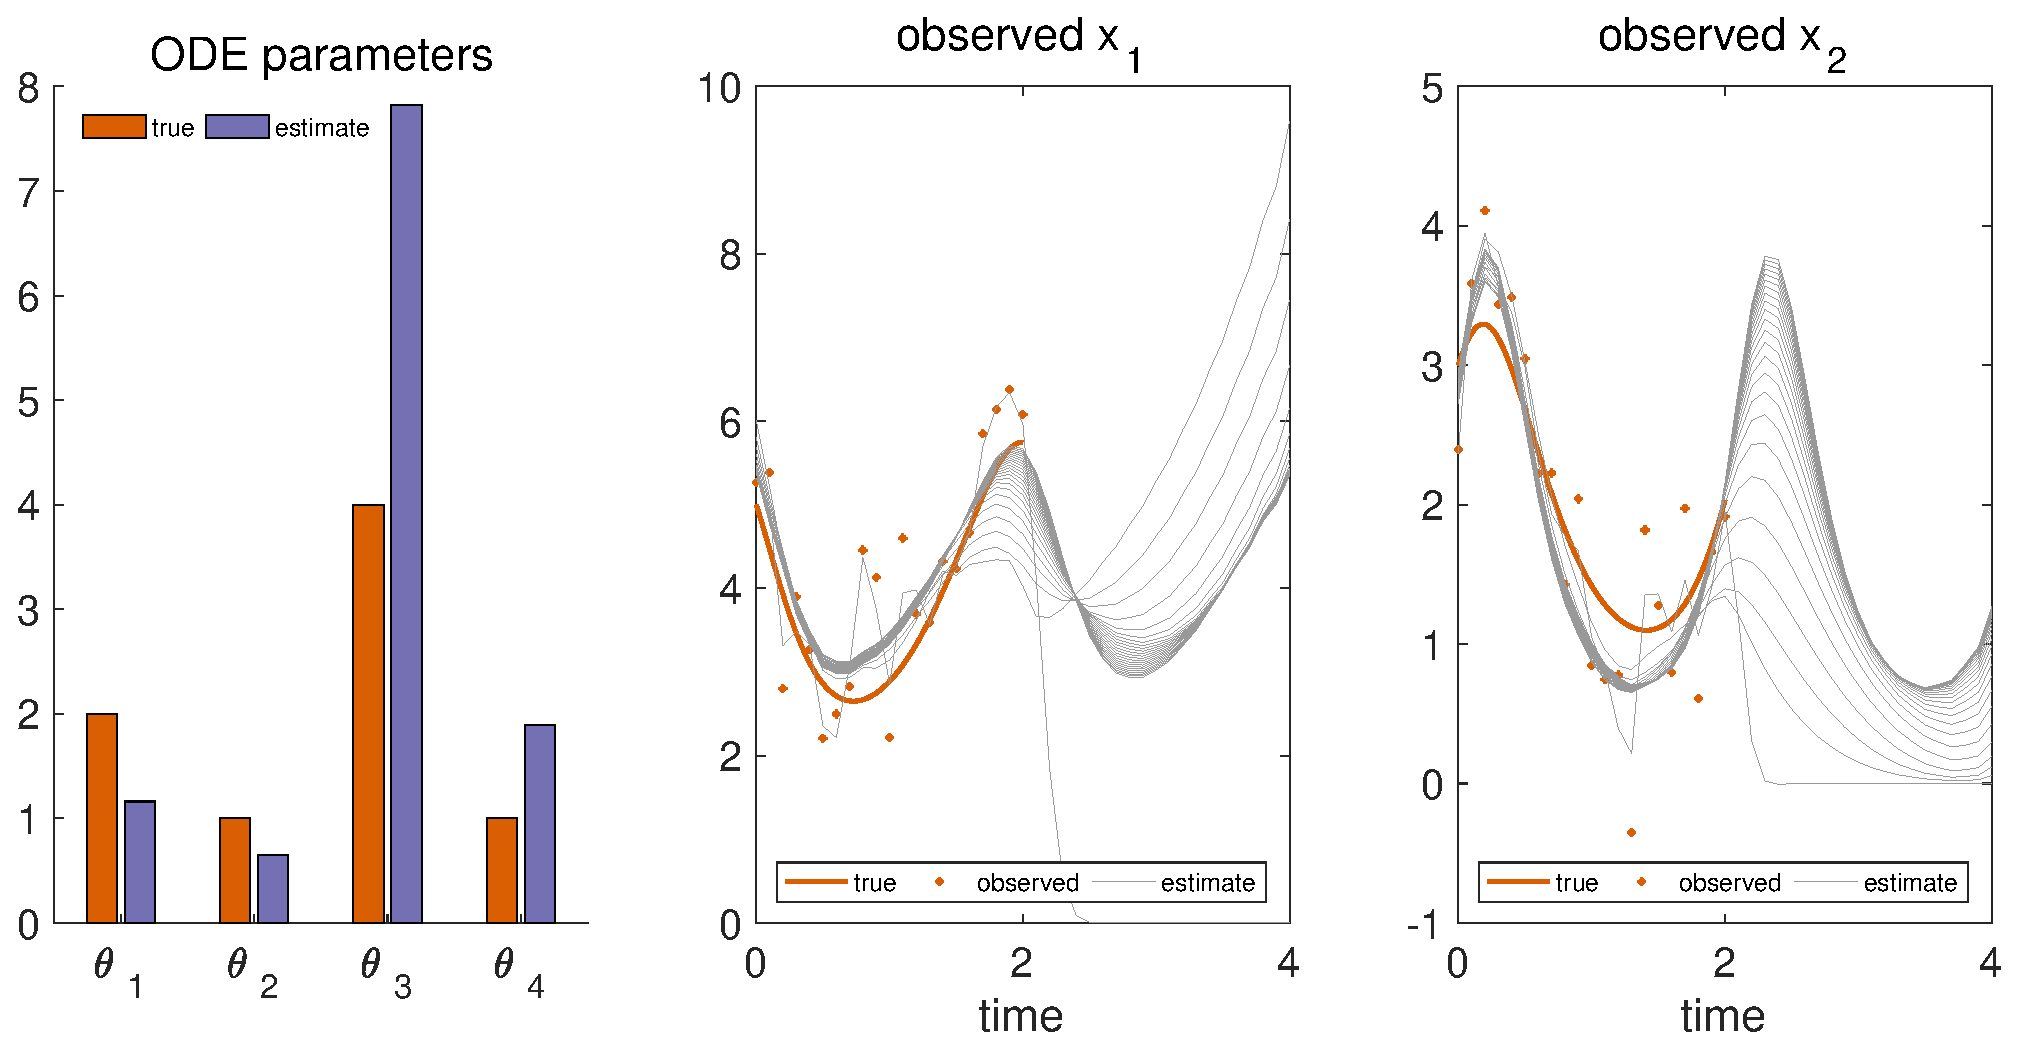
\includegraphics [width=5in]{VGM_for_Lotka_Volterra_25.eps}

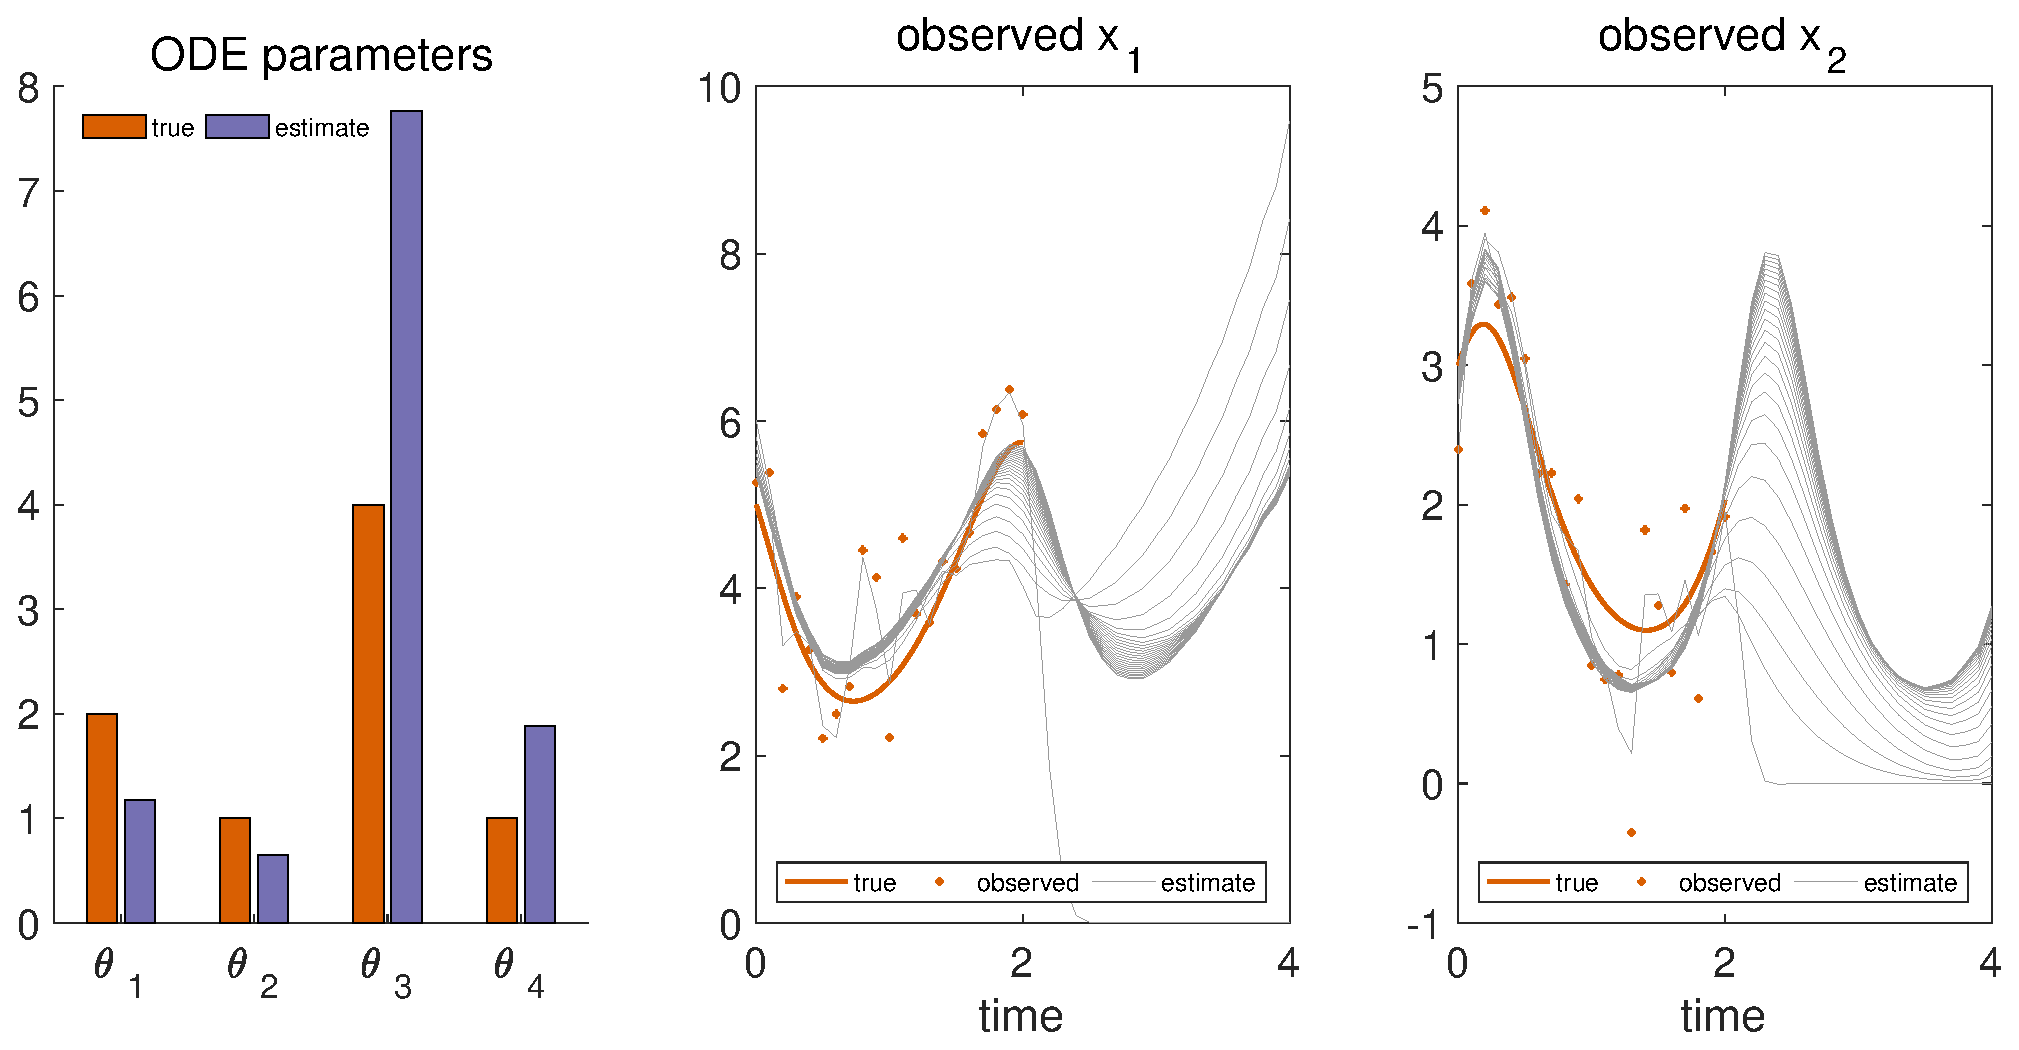
\includegraphics [width=5in]{VGM_for_Lotka_Volterra_26.eps}

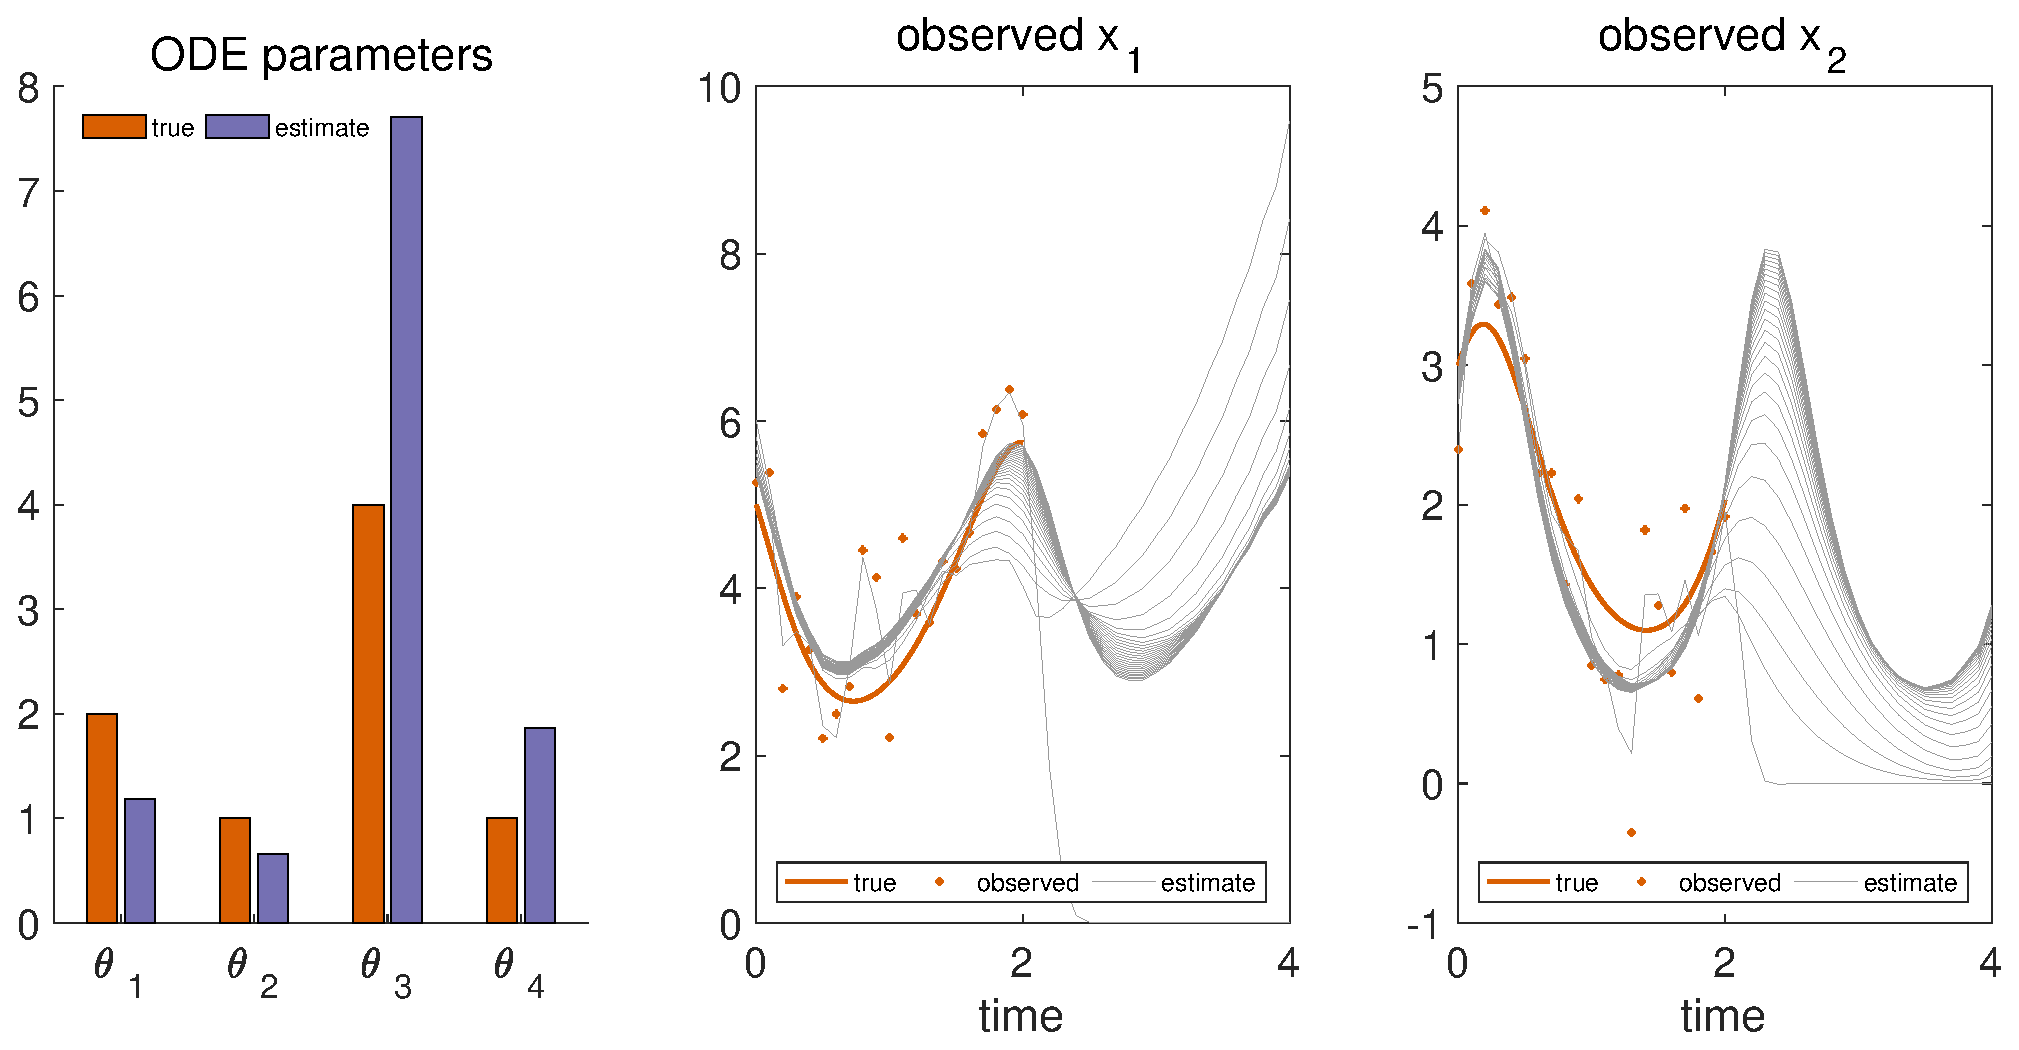
\includegraphics [width=5in]{VGM_for_Lotka_Volterra_27.eps}

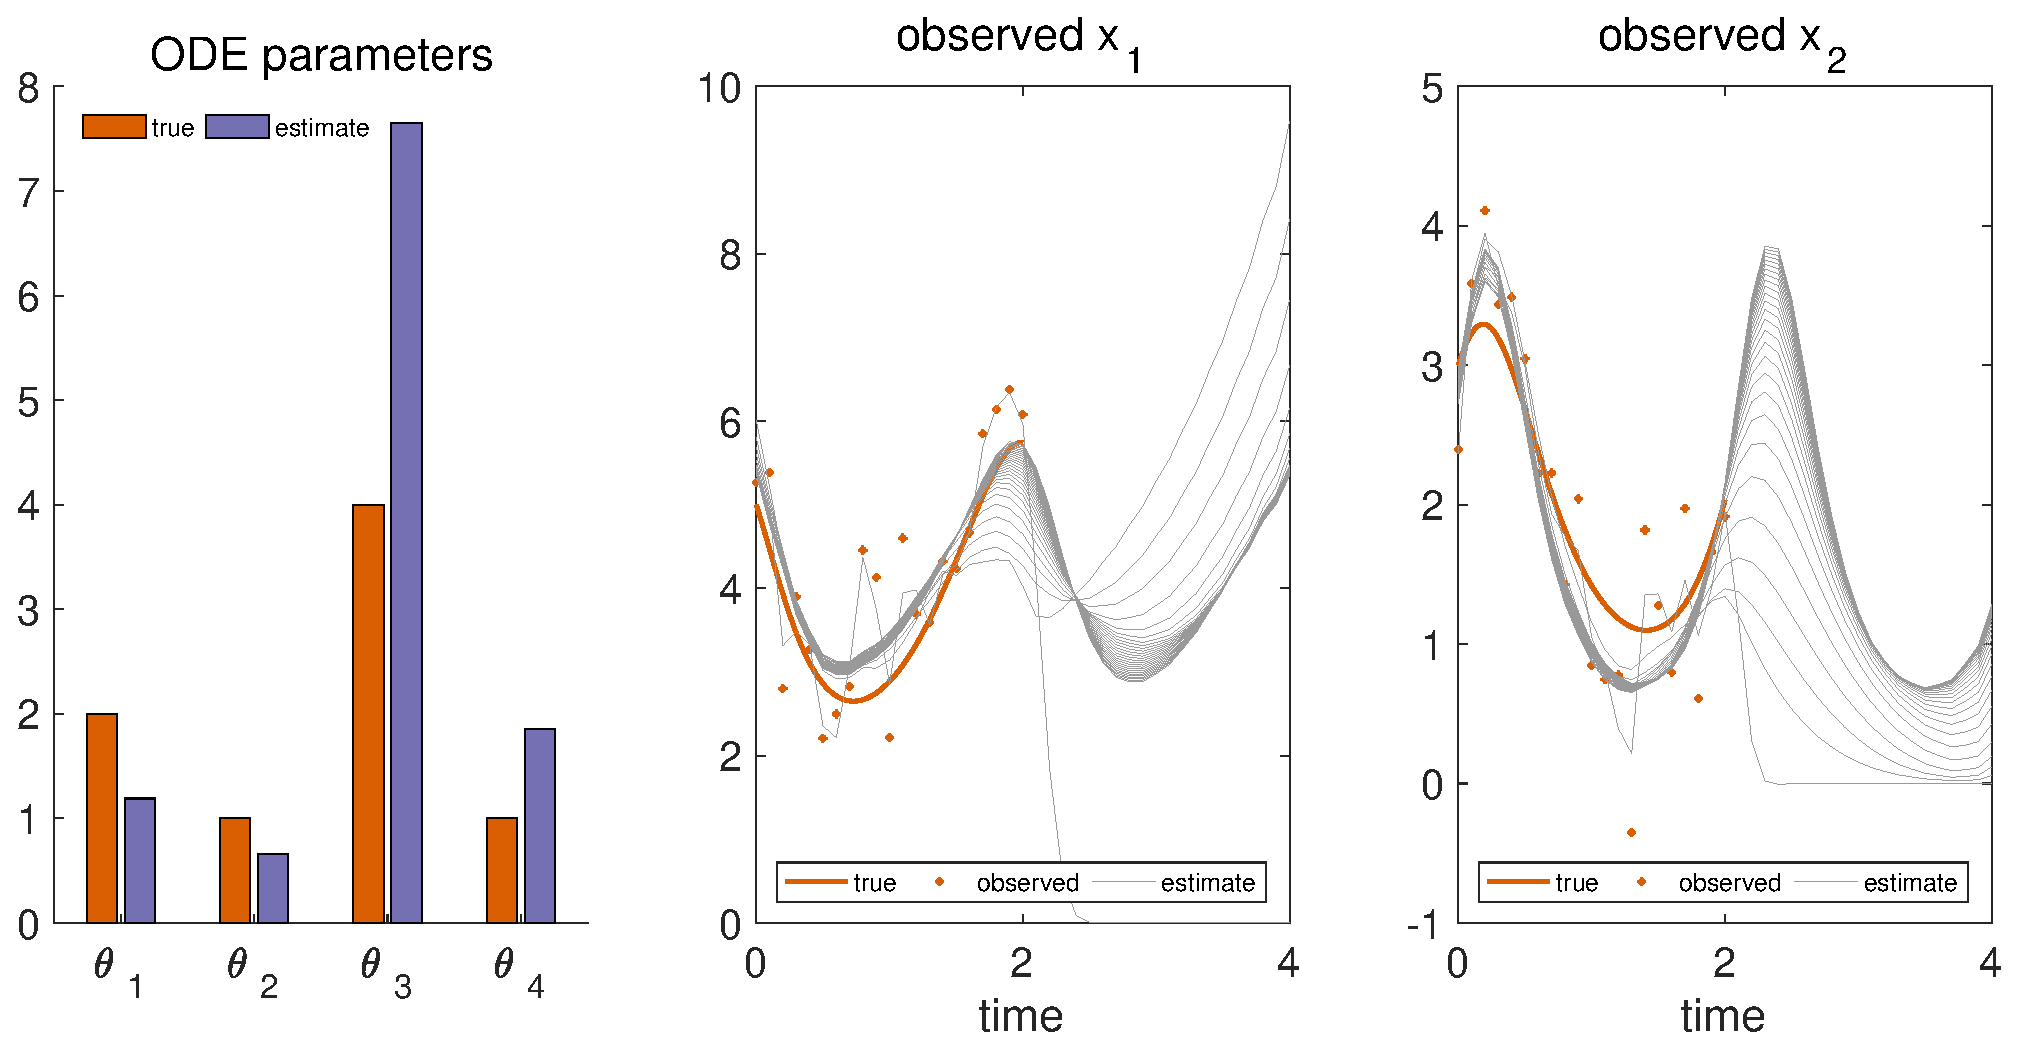
\includegraphics [width=5in]{VGM_for_Lotka_Volterra_28.eps}

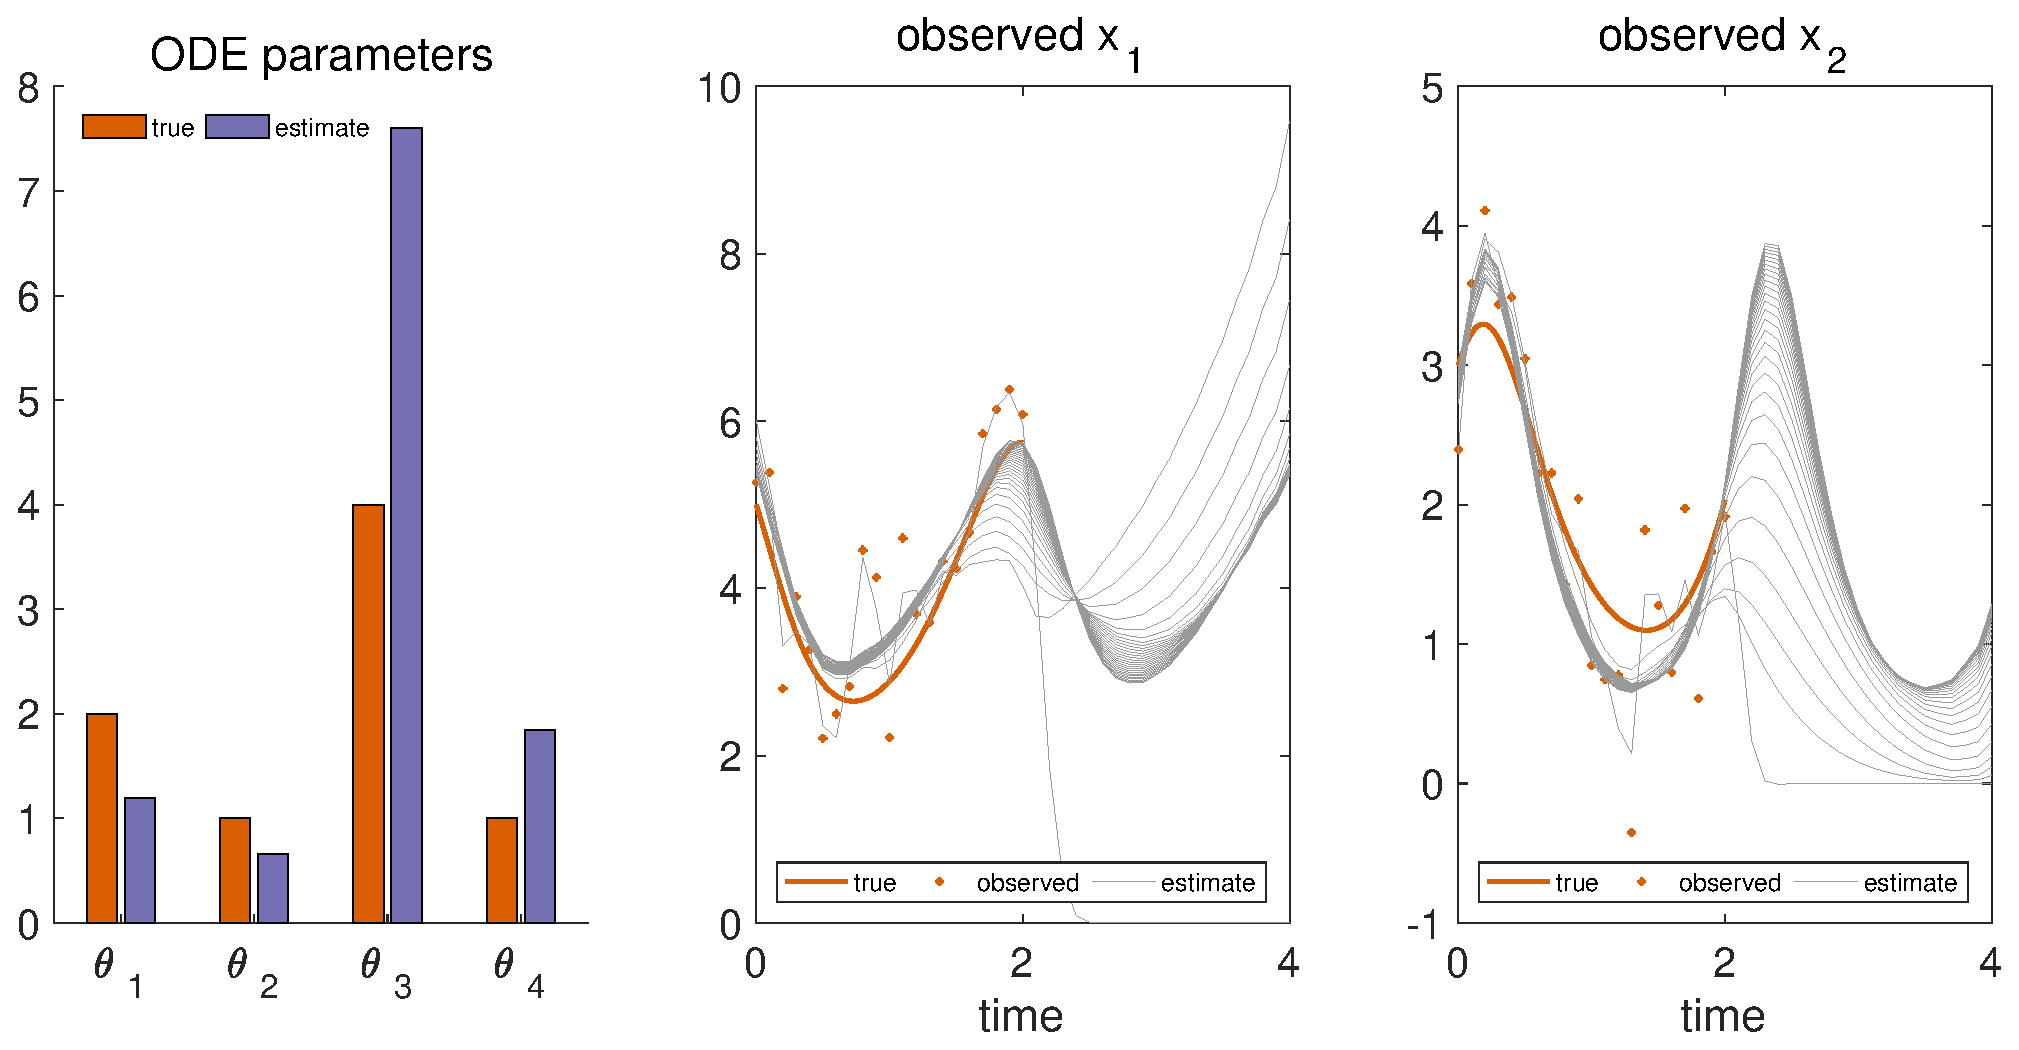
\includegraphics [width=5in]{VGM_for_Lotka_Volterra_29.eps}

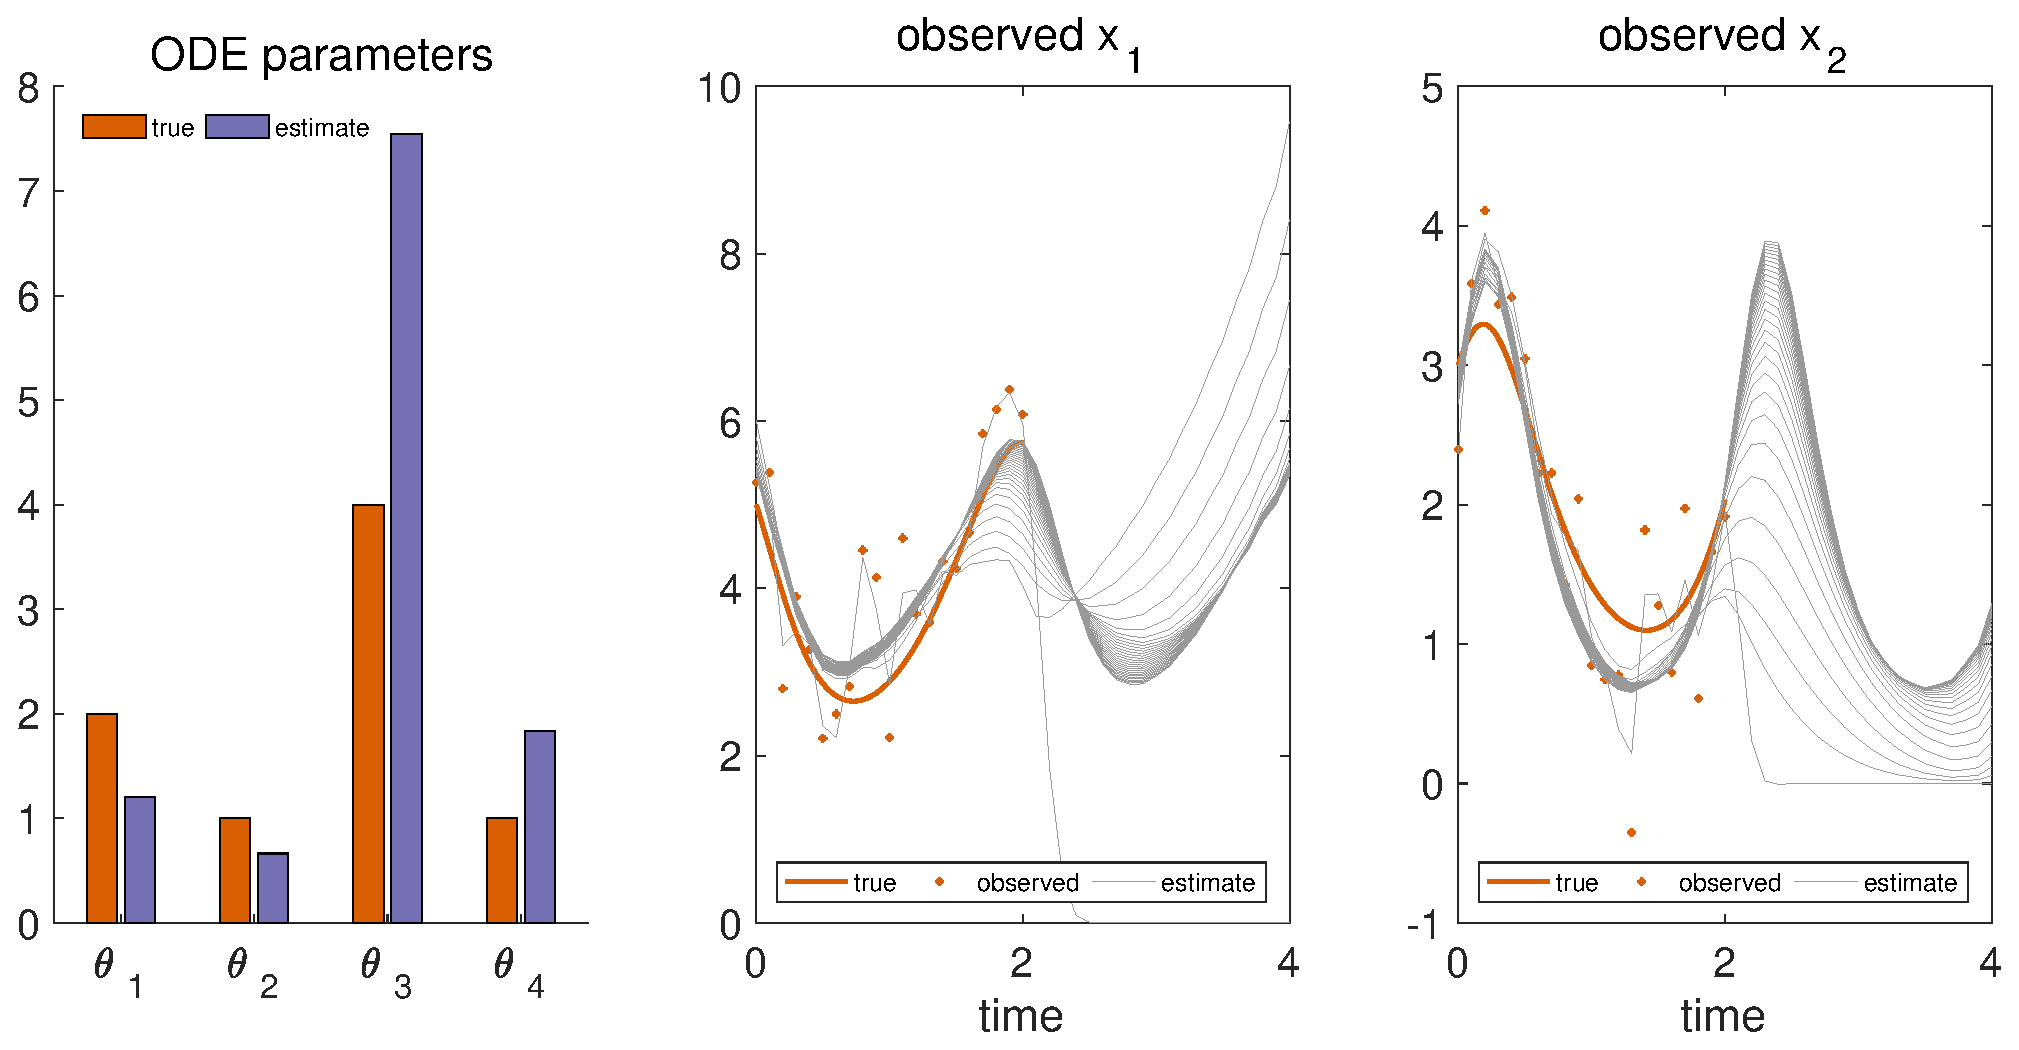
\includegraphics [width=5in]{VGM_for_Lotka_Volterra_30.eps}

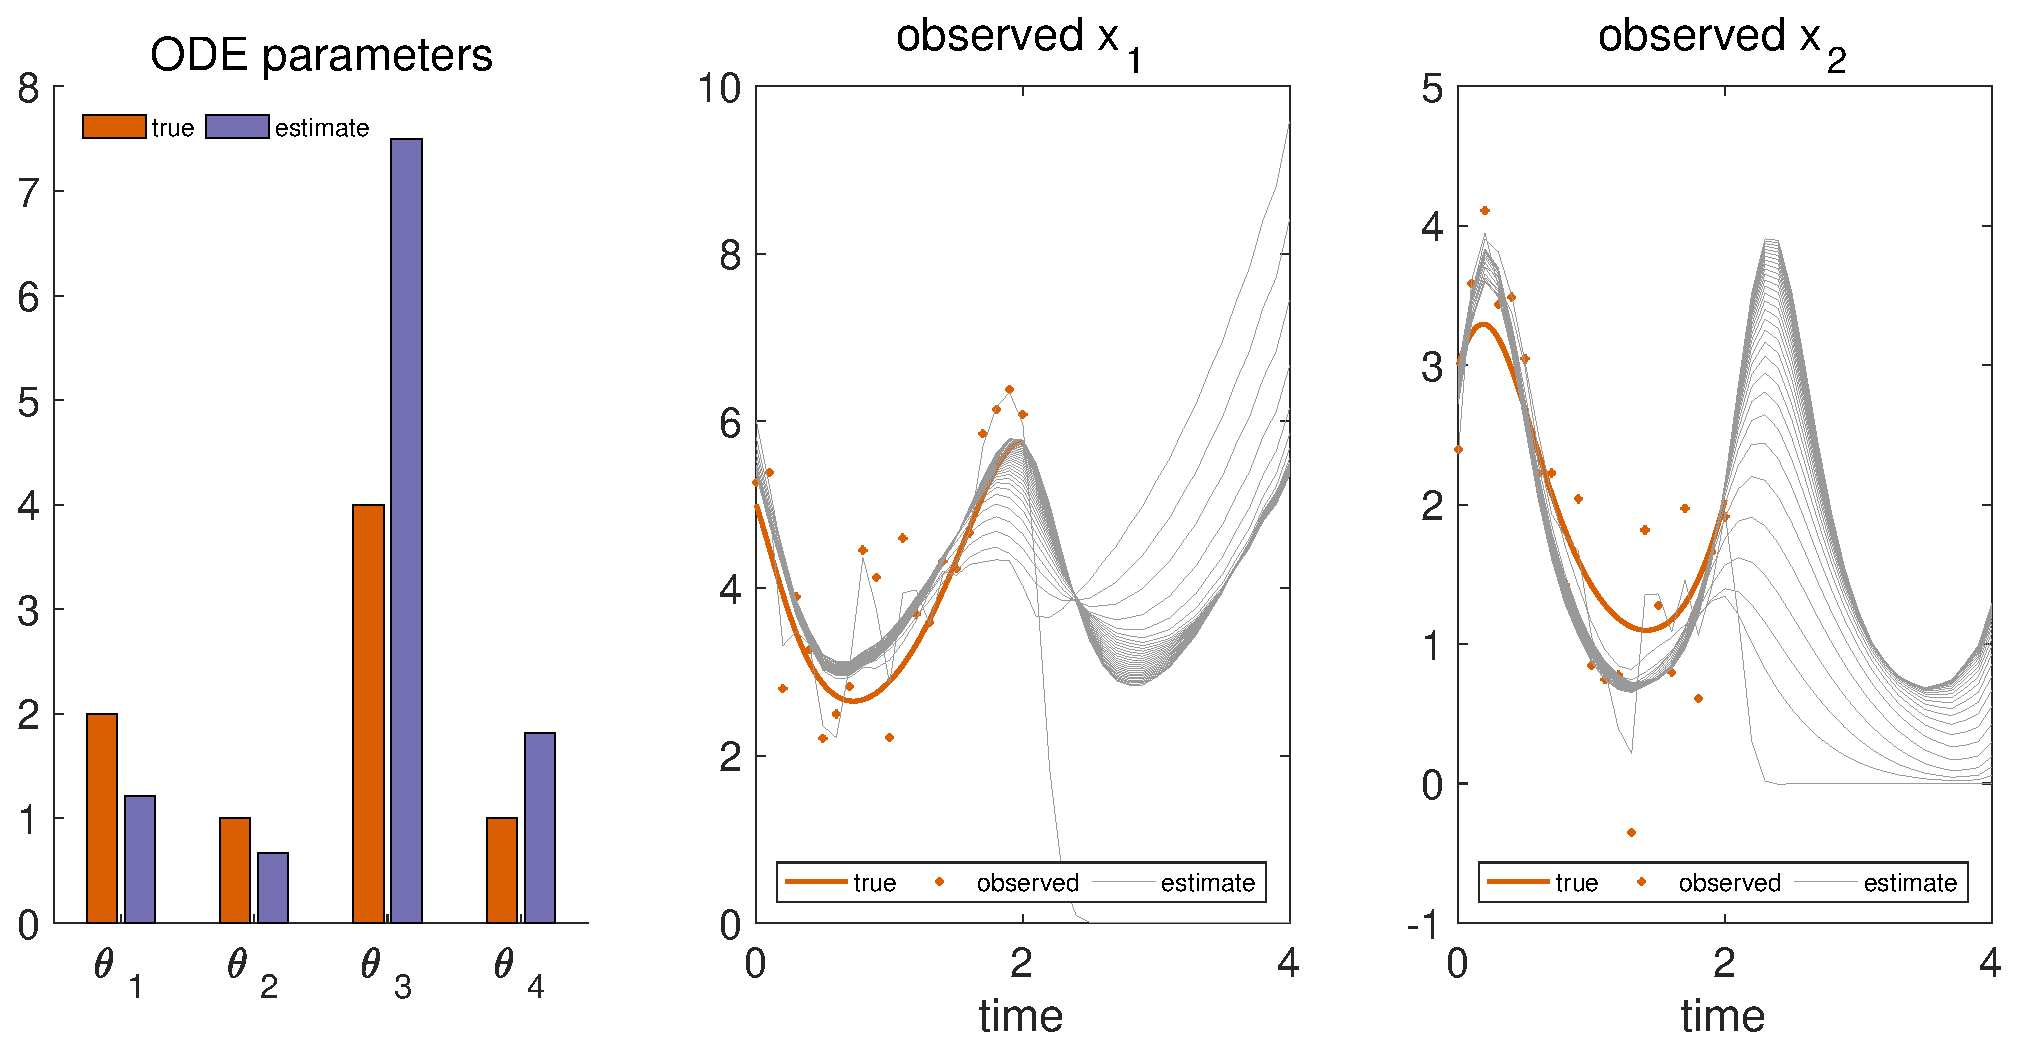
\includegraphics [width=5in]{VGM_for_Lotka_Volterra_31.eps}

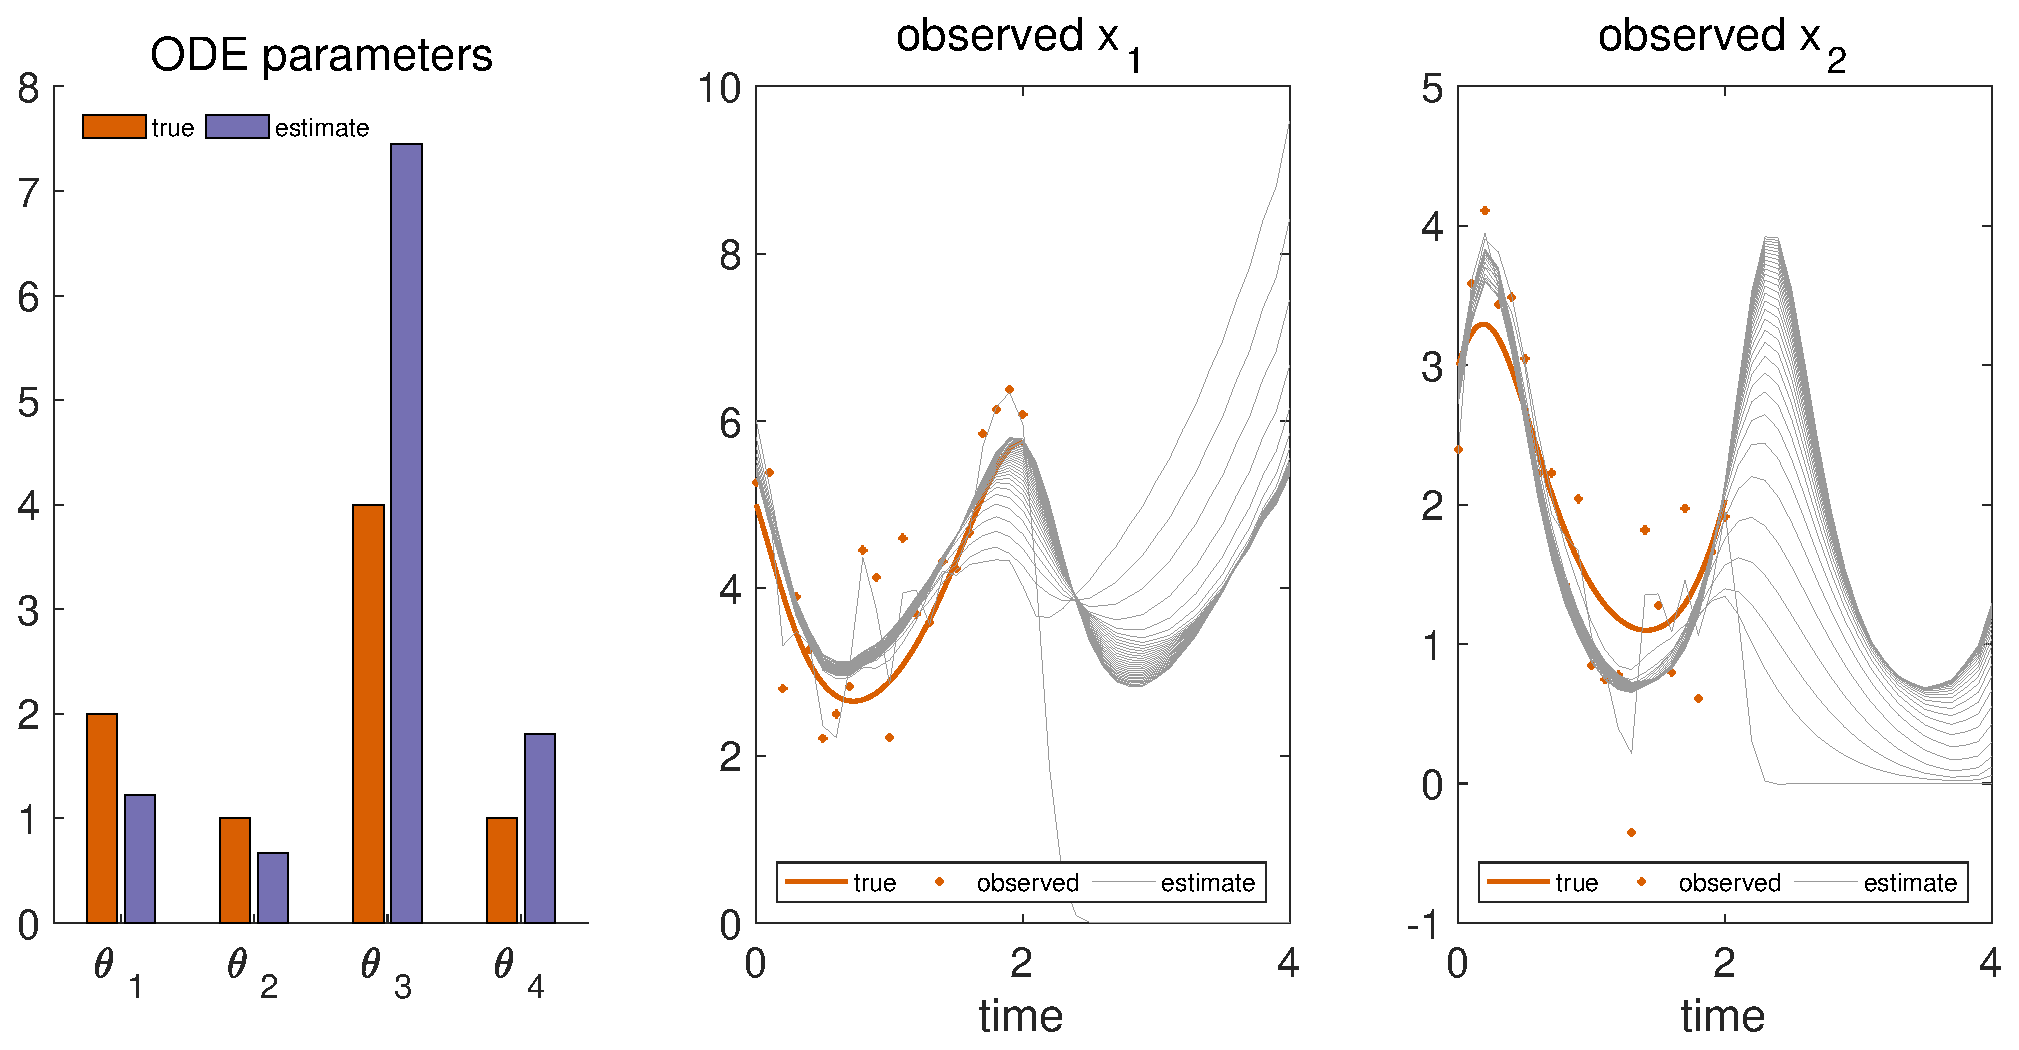
\includegraphics [width=5in]{VGM_for_Lotka_Volterra_32.eps}

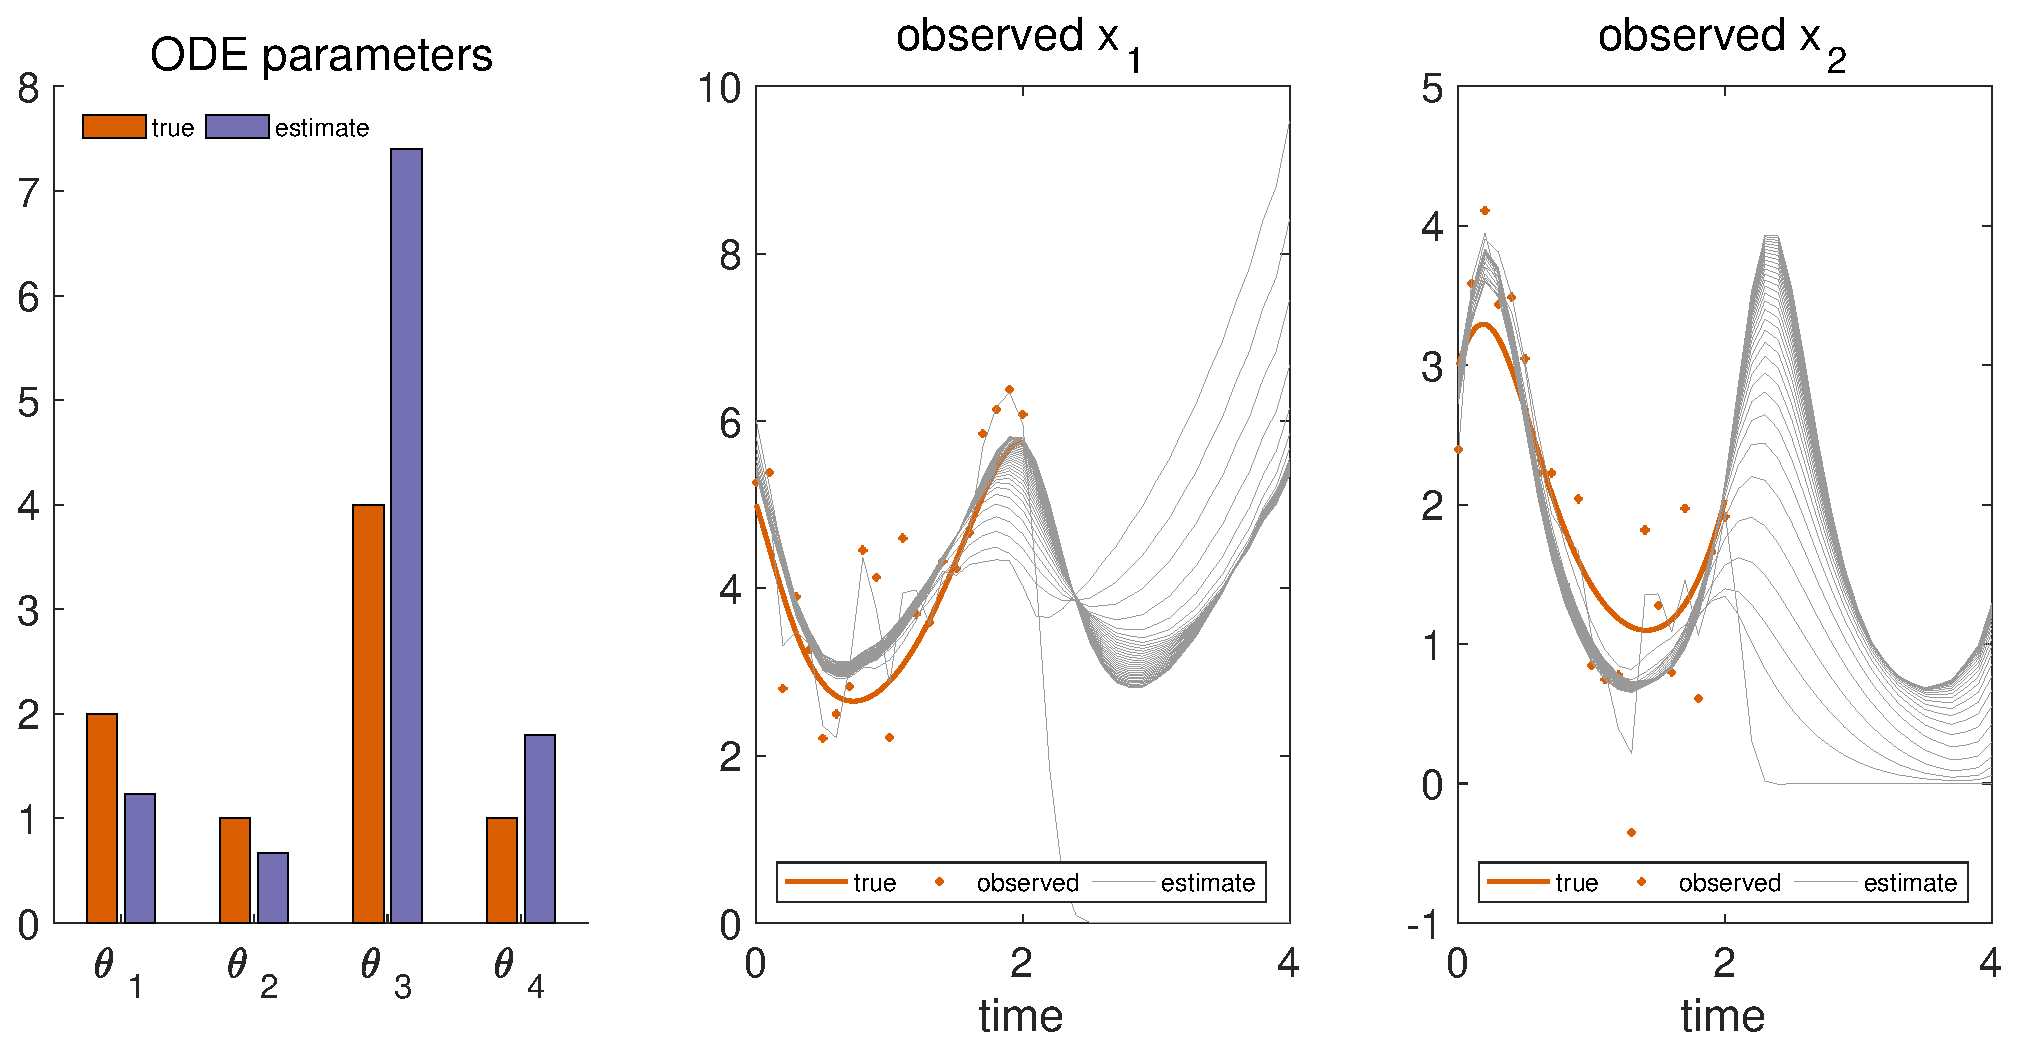
\includegraphics [width=5in]{VGM_for_Lotka_Volterra_33.eps}

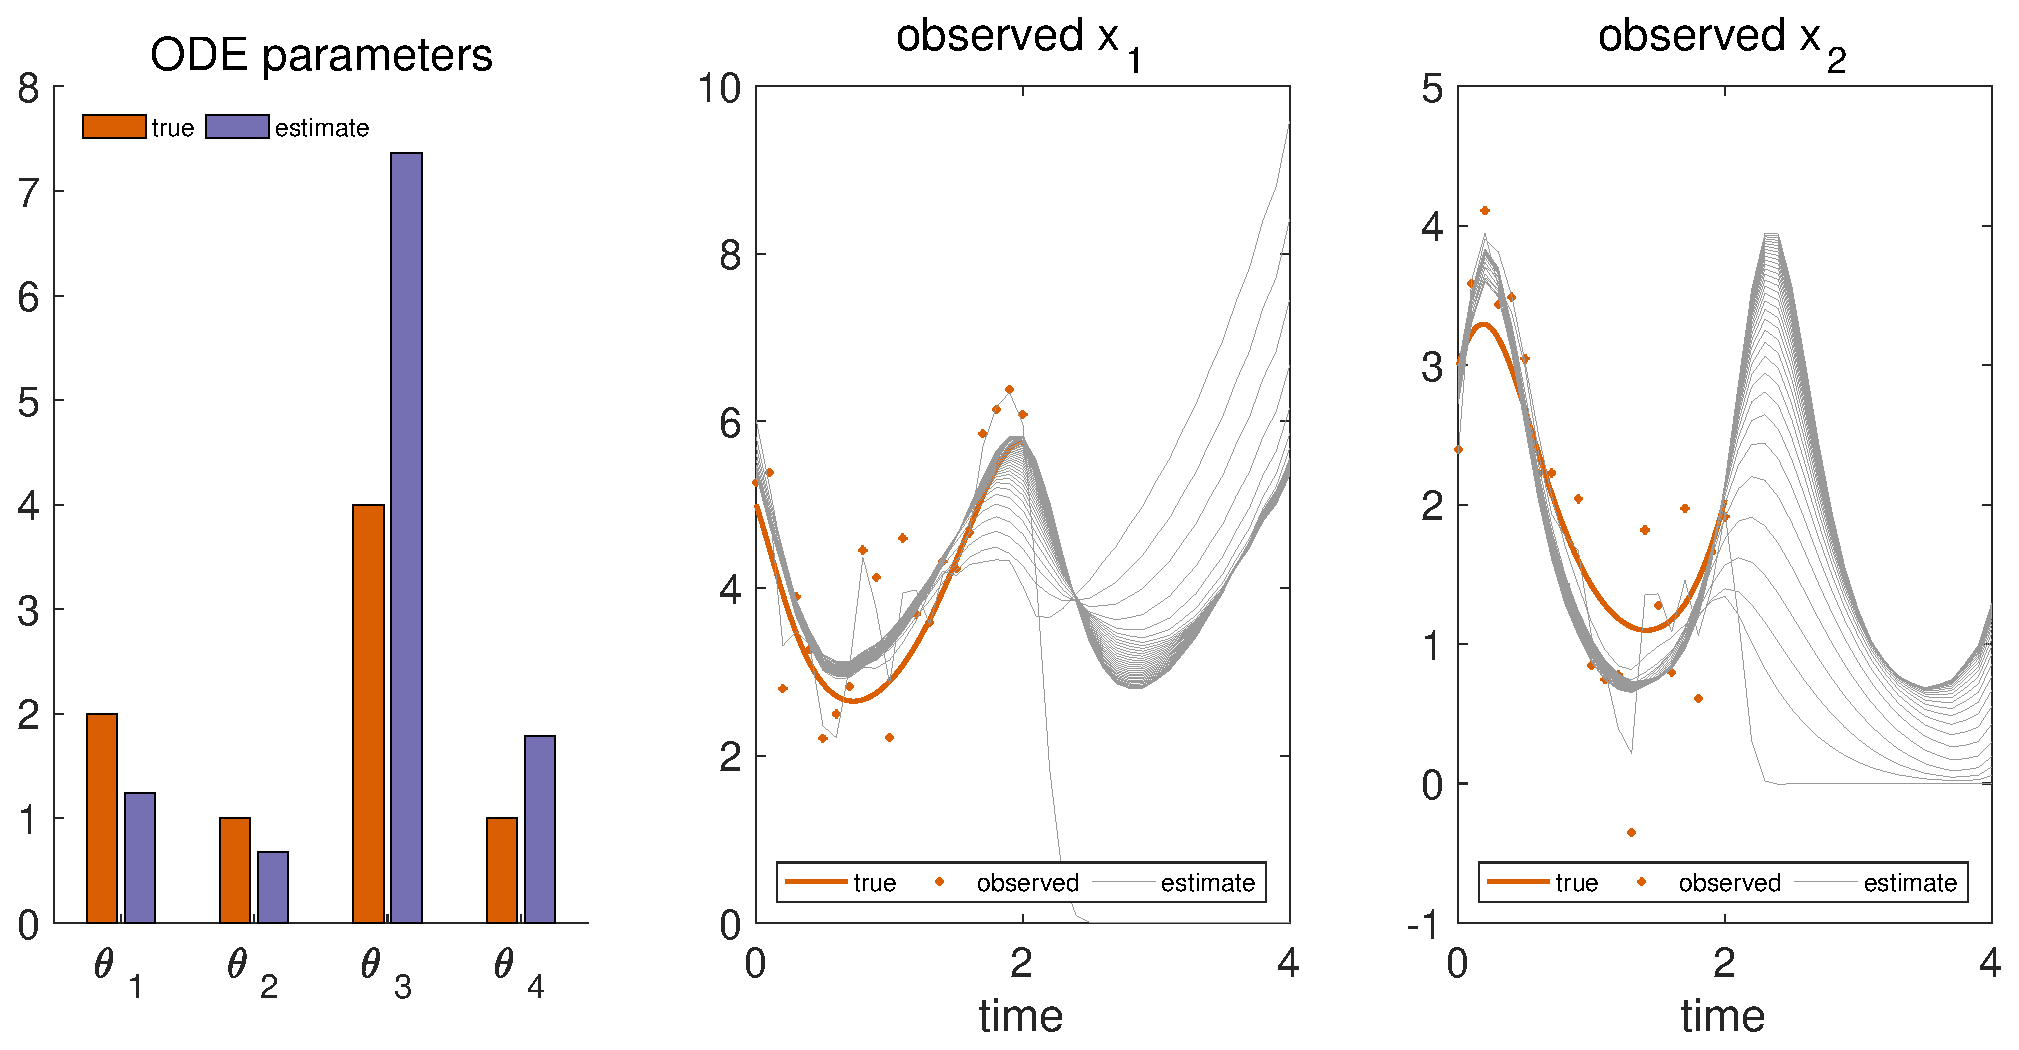
\includegraphics [width=5in]{VGM_for_Lotka_Volterra_34.eps}

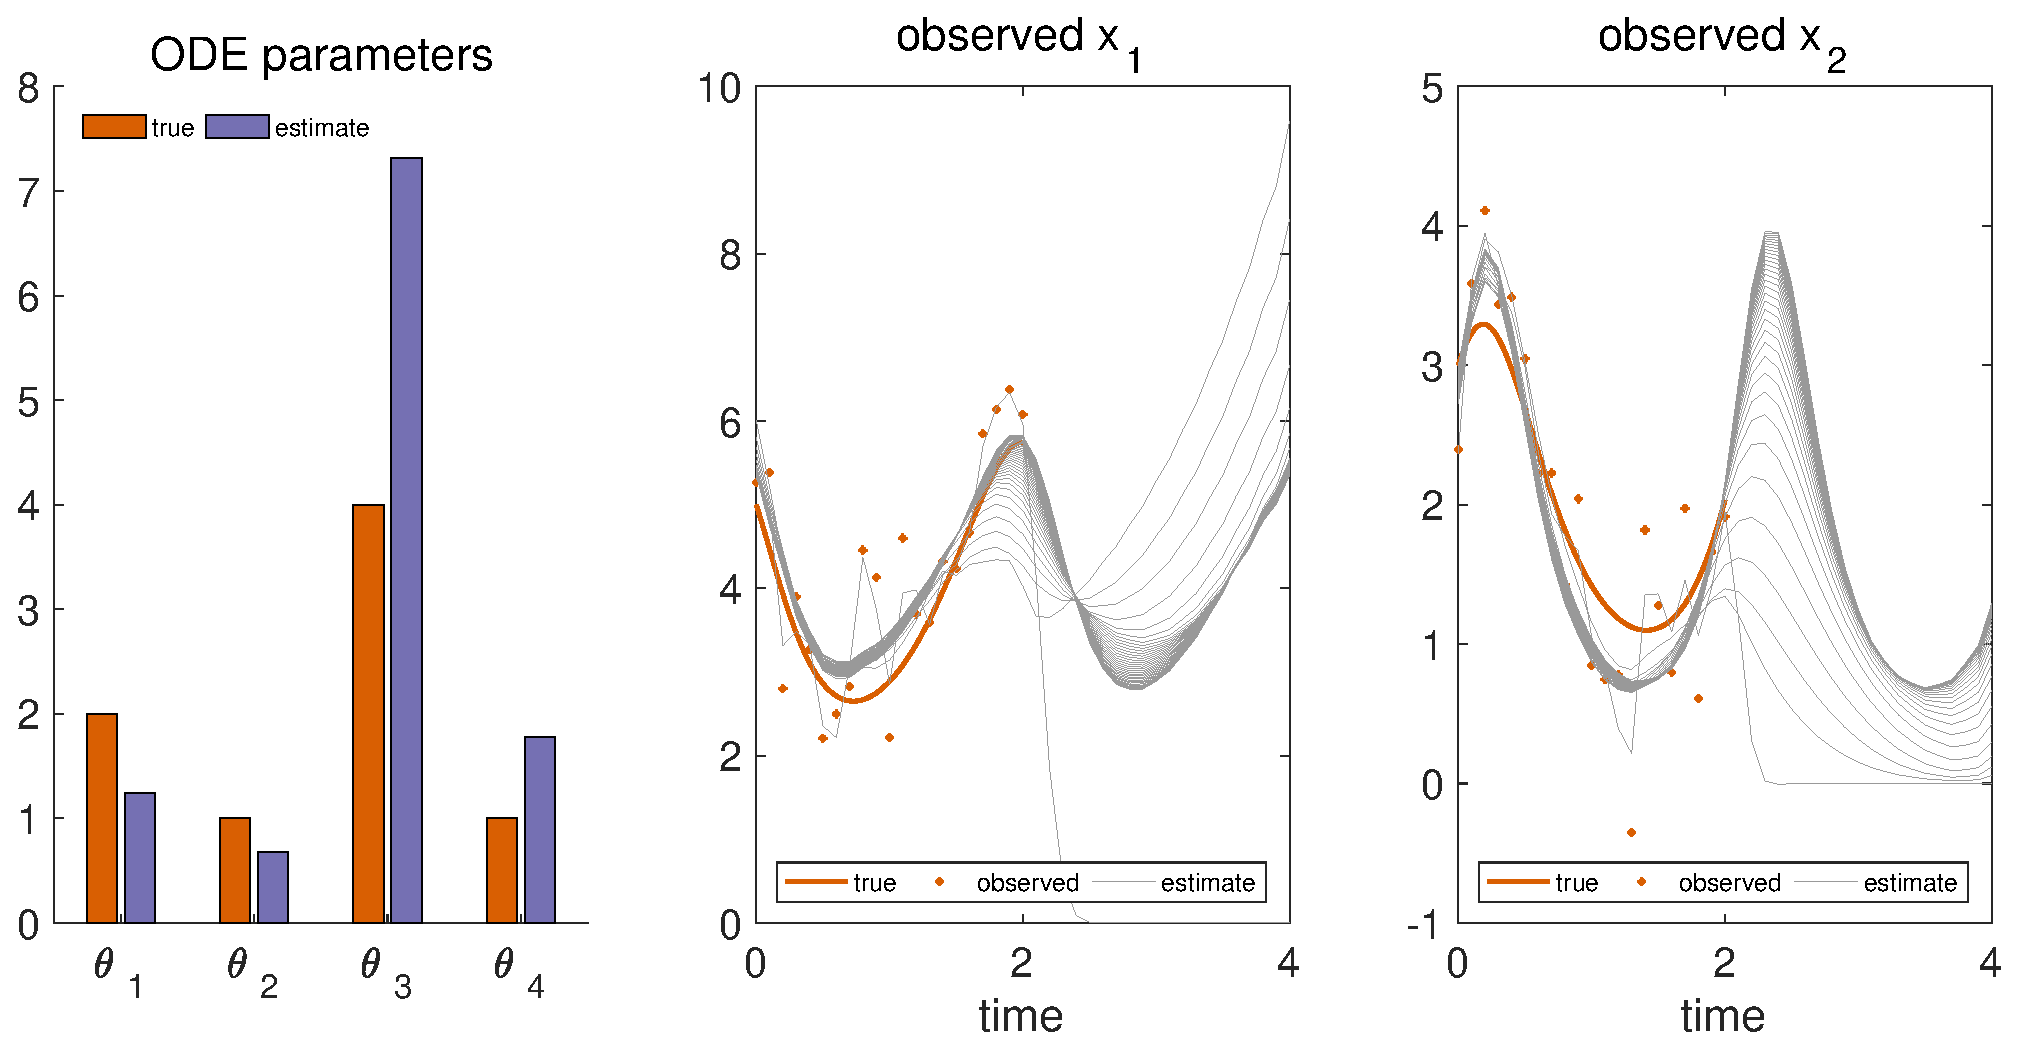
\includegraphics [width=5in]{VGM_for_Lotka_Volterra_35.eps}

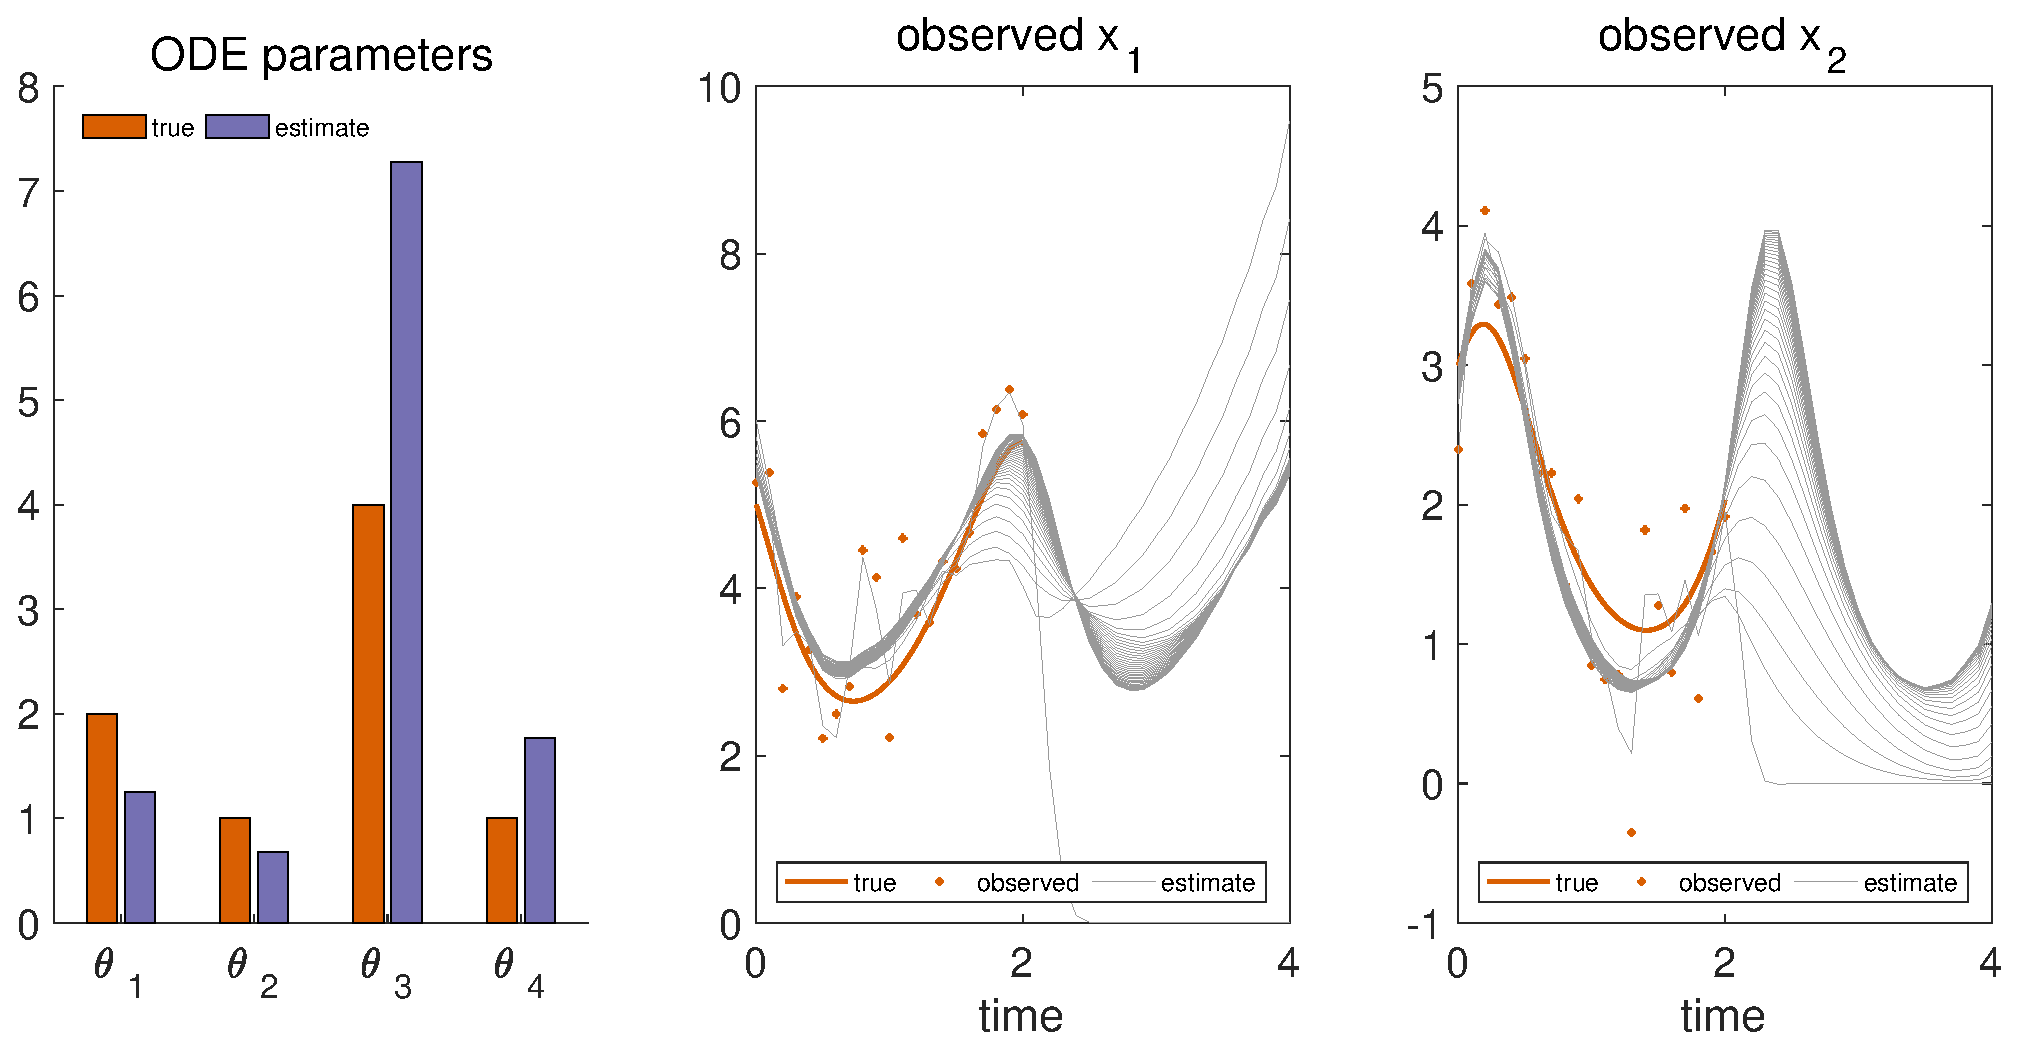
\includegraphics [width=5in]{VGM_for_Lotka_Volterra_36.eps}

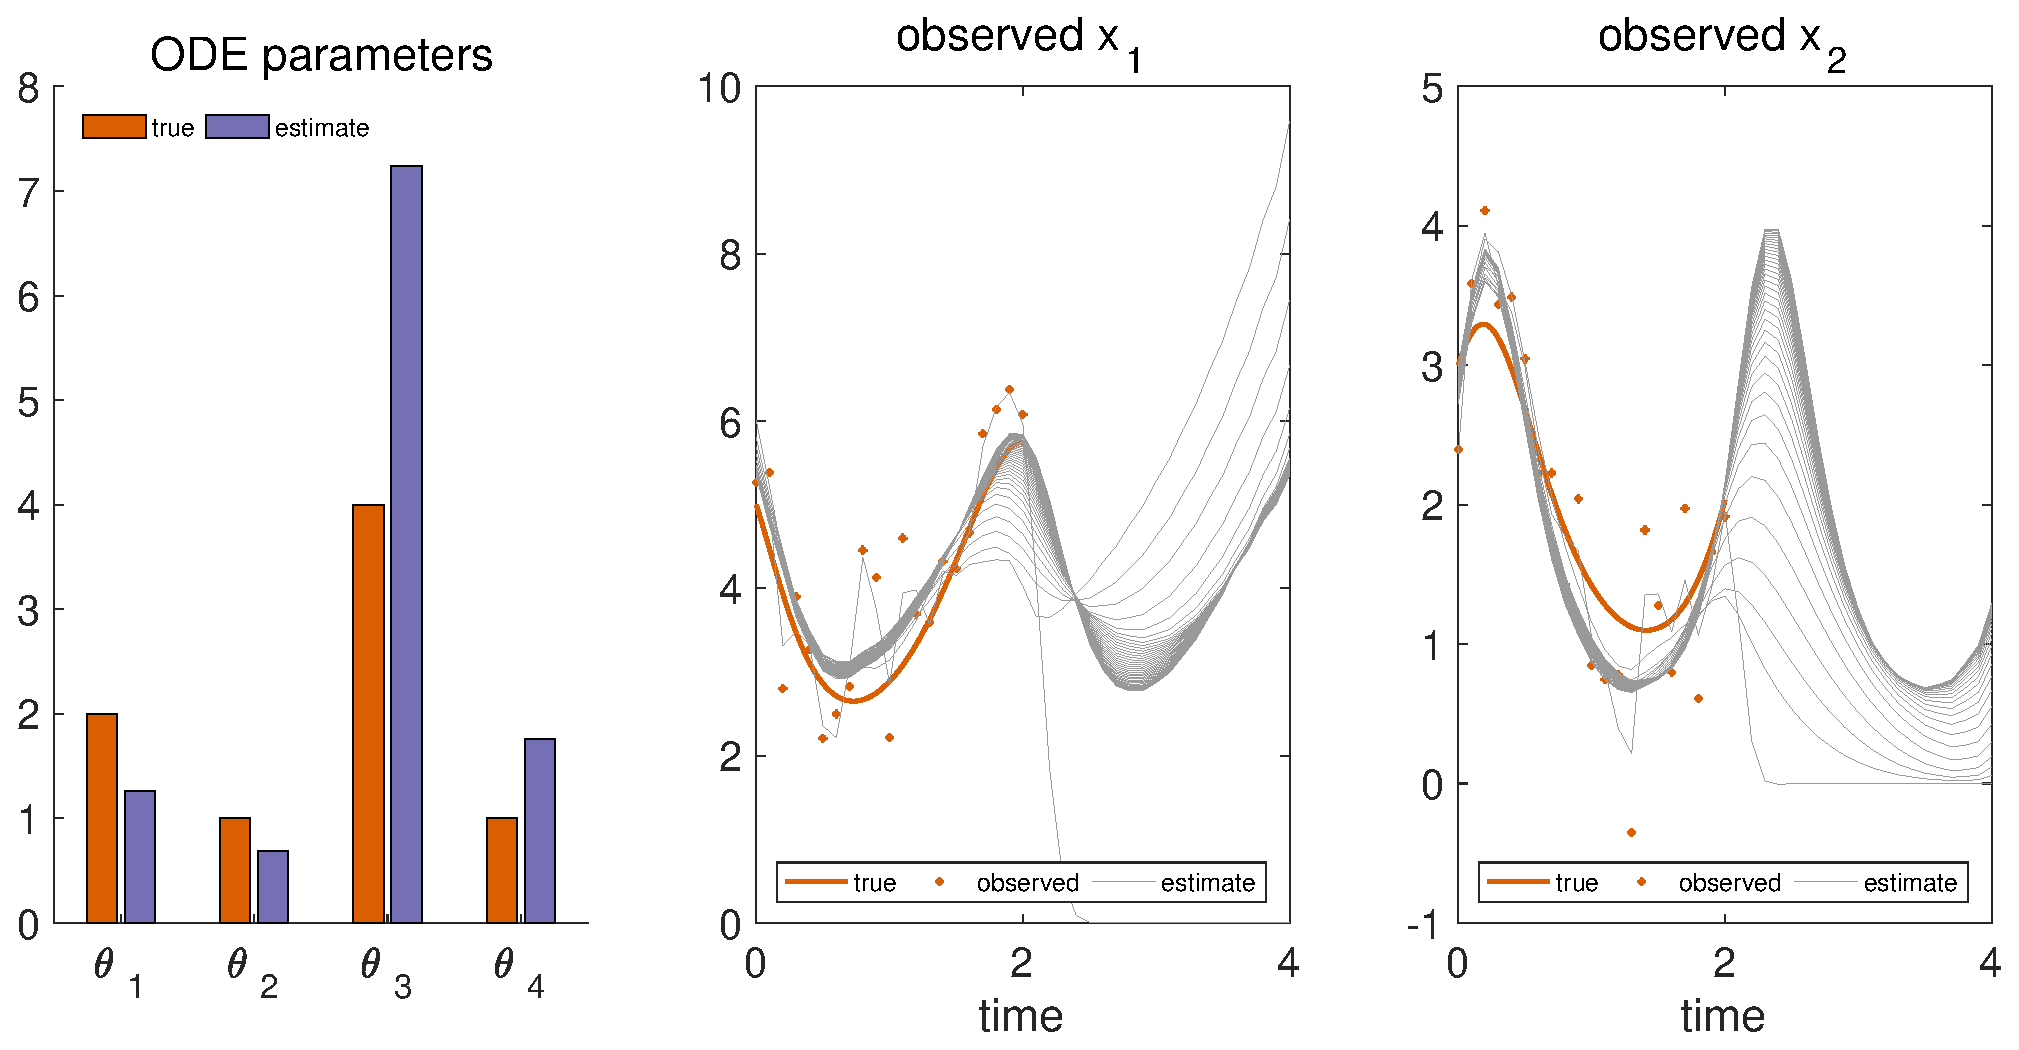
\includegraphics [width=5in]{VGM_for_Lotka_Volterra_37.eps}

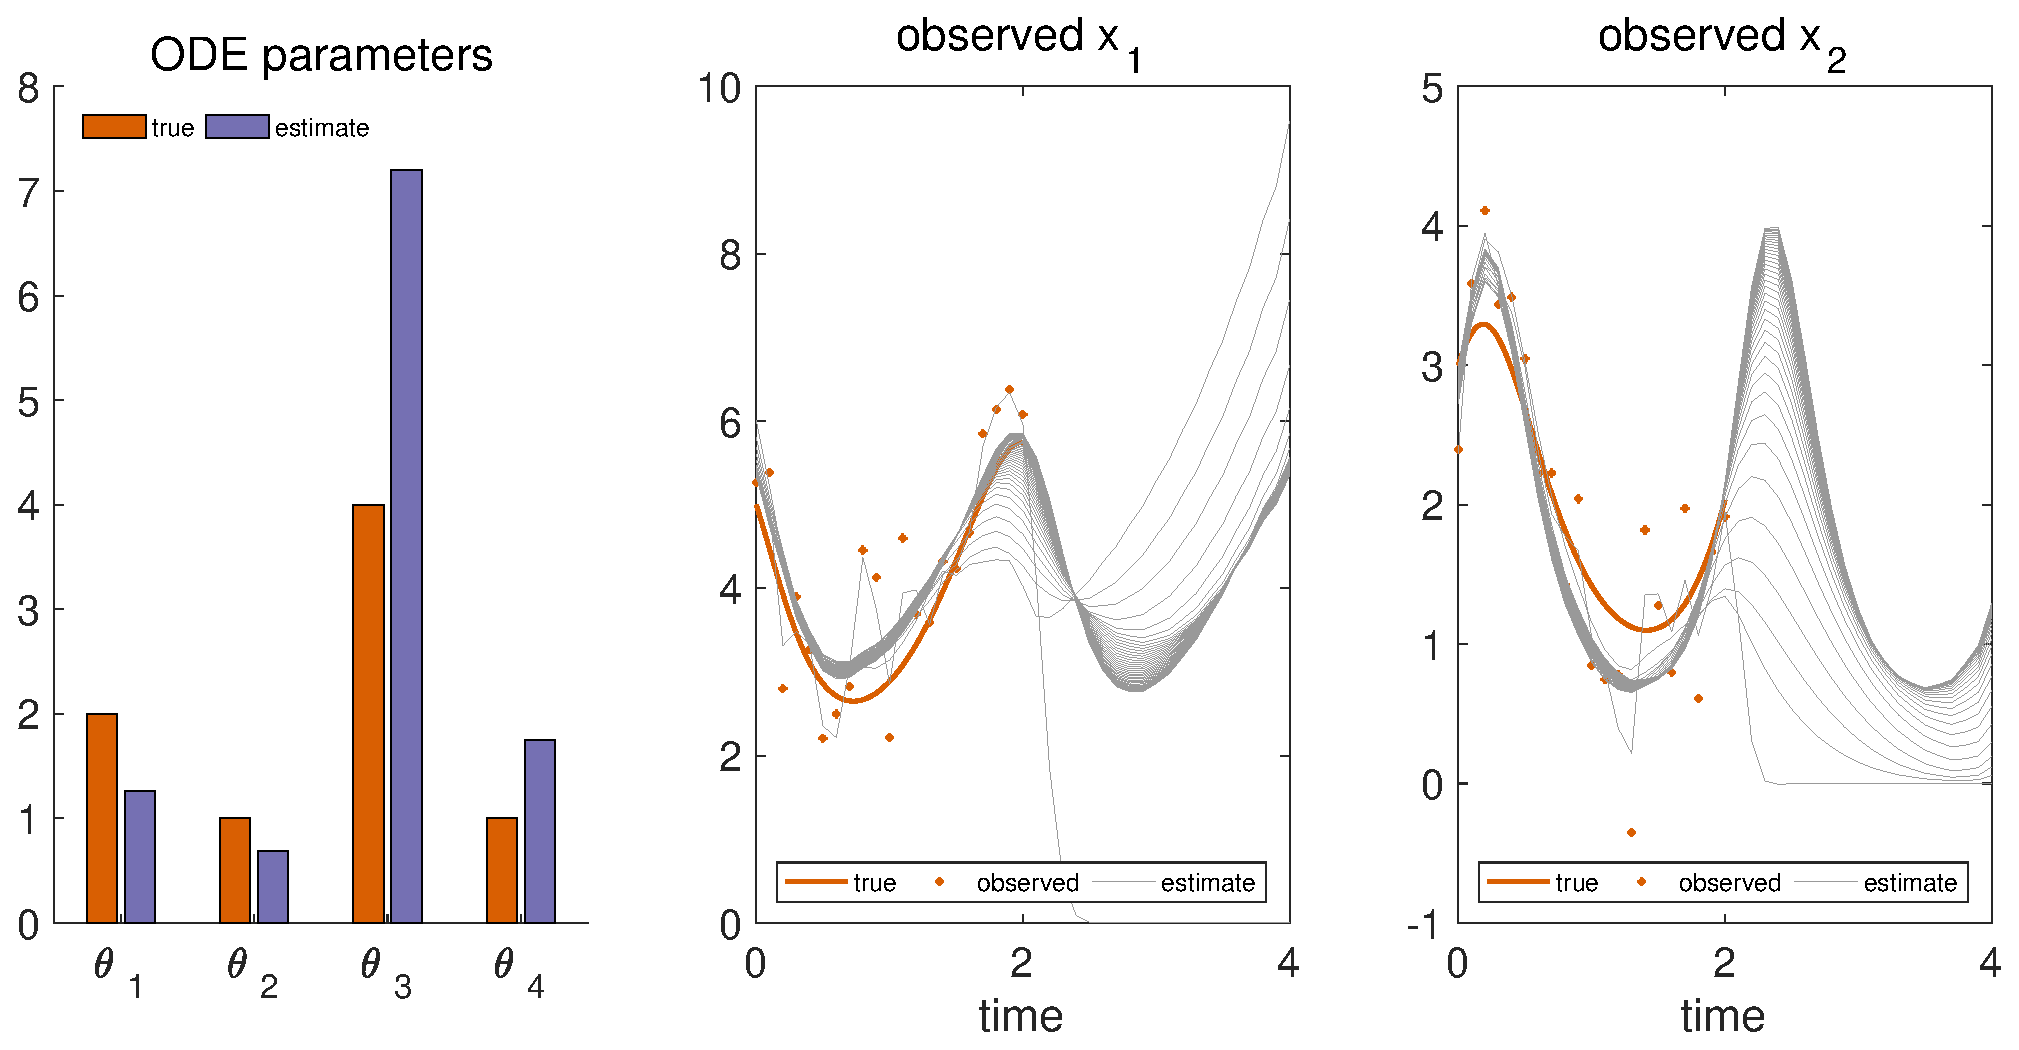
\includegraphics [width=5in]{VGM_for_Lotka_Volterra_38.eps}

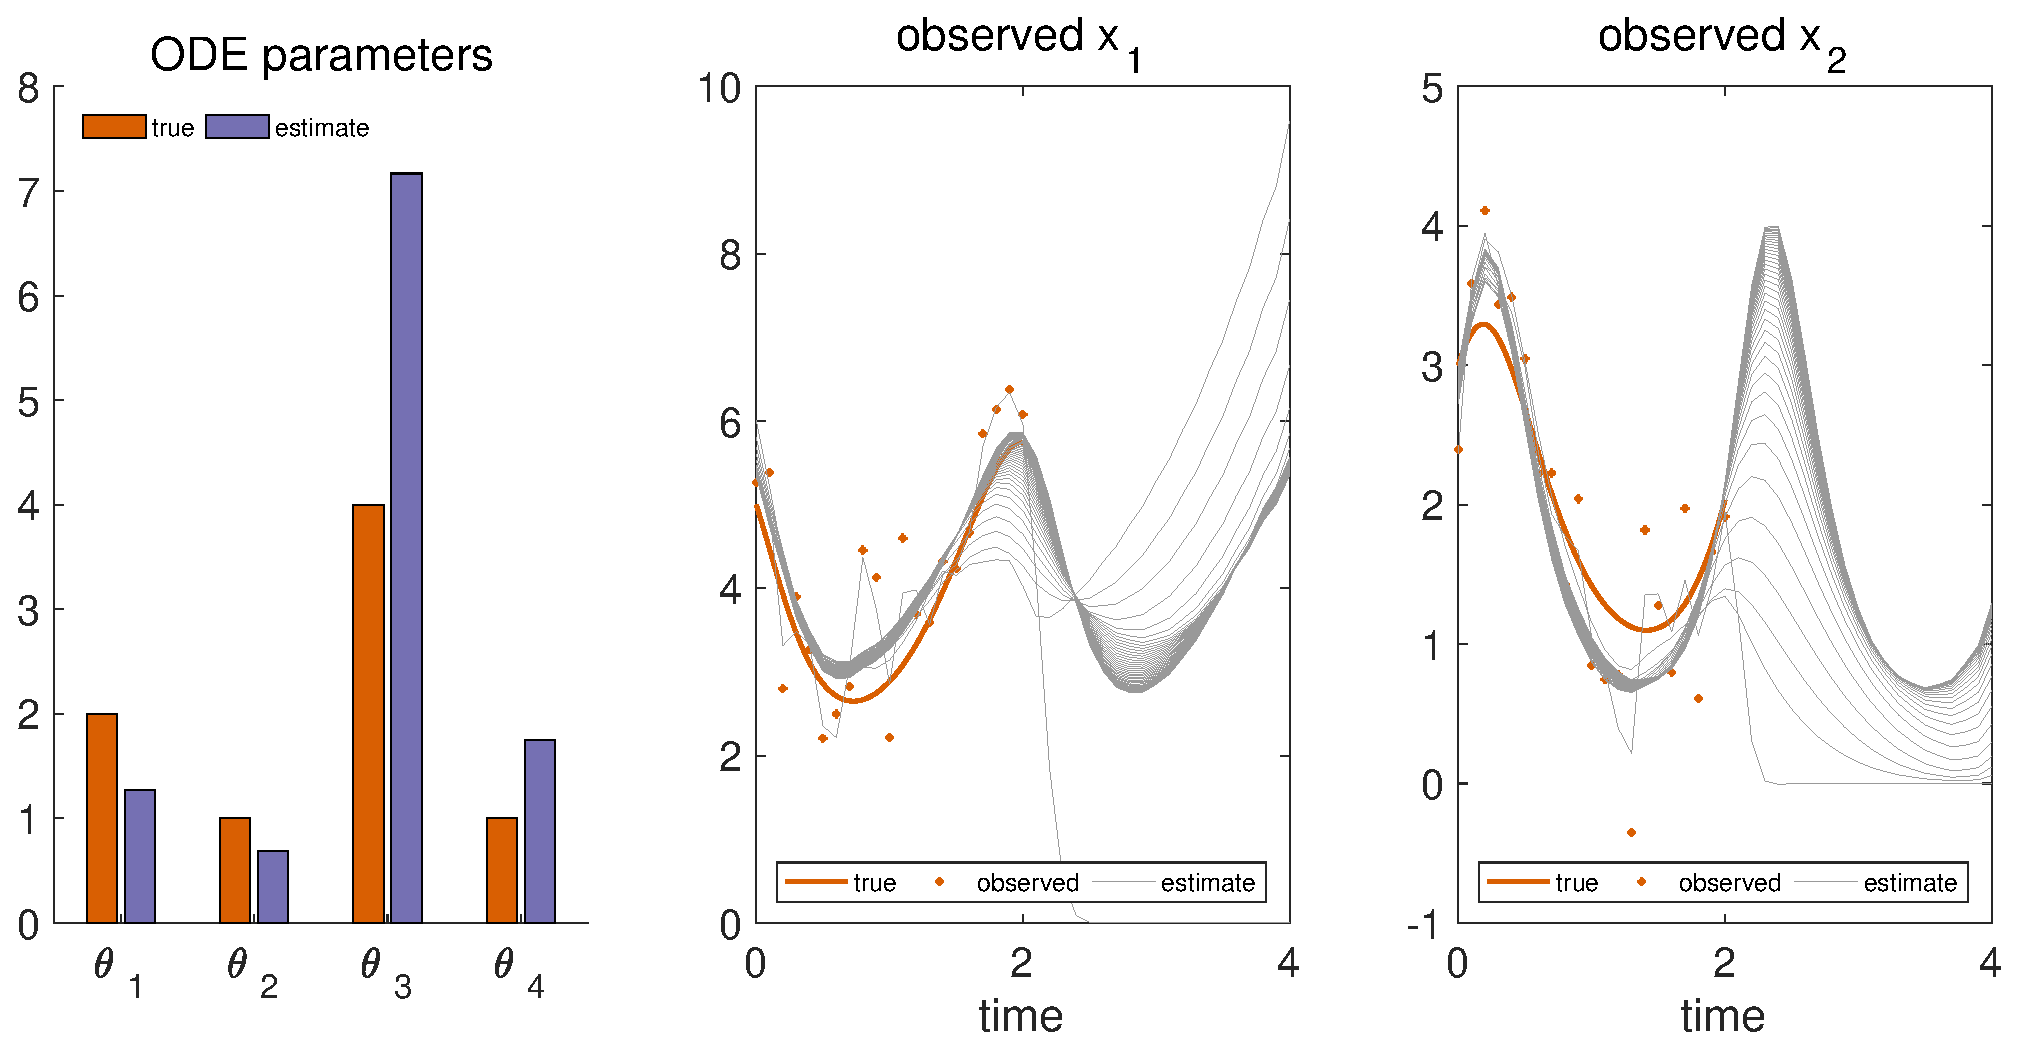
\includegraphics [width=5in]{VGM_for_Lotka_Volterra_39.eps}

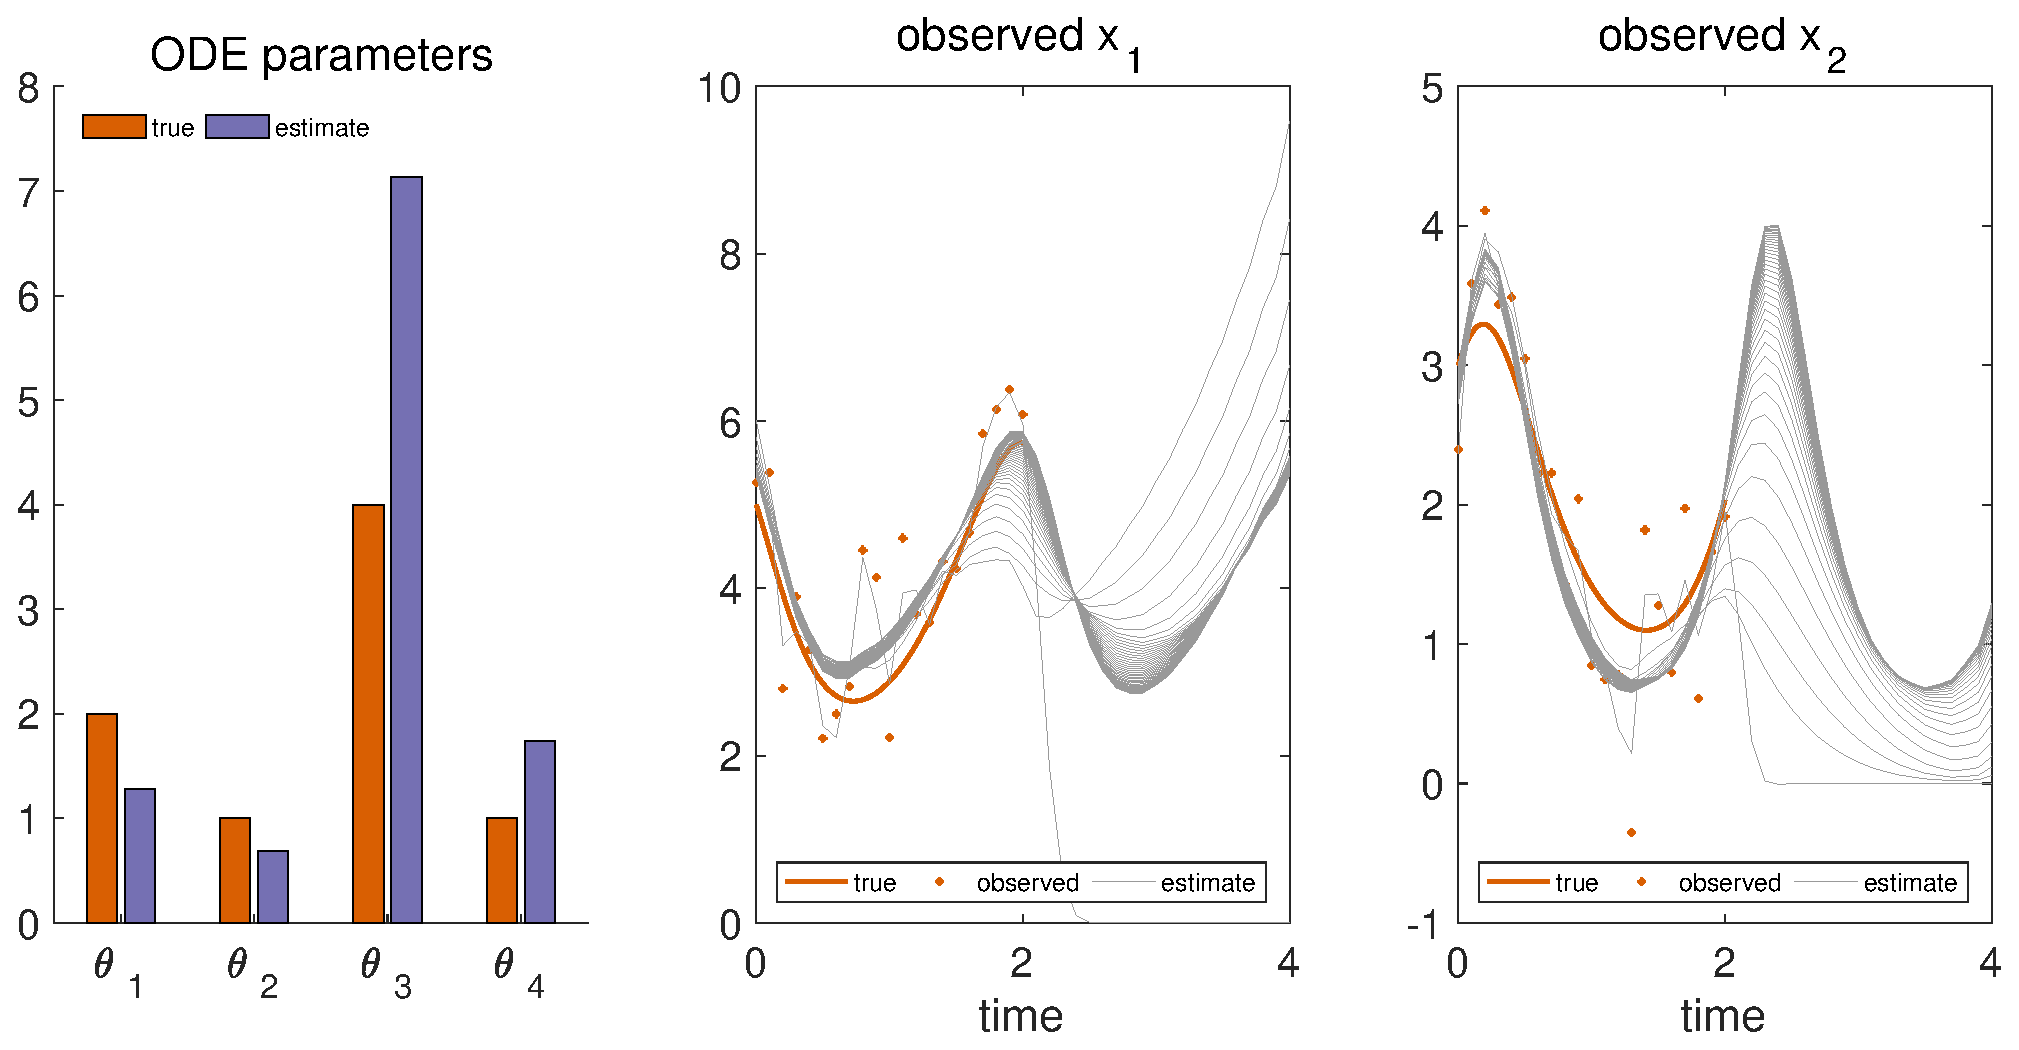
\includegraphics [width=5in]{VGM_for_Lotka_Volterra_40.eps}

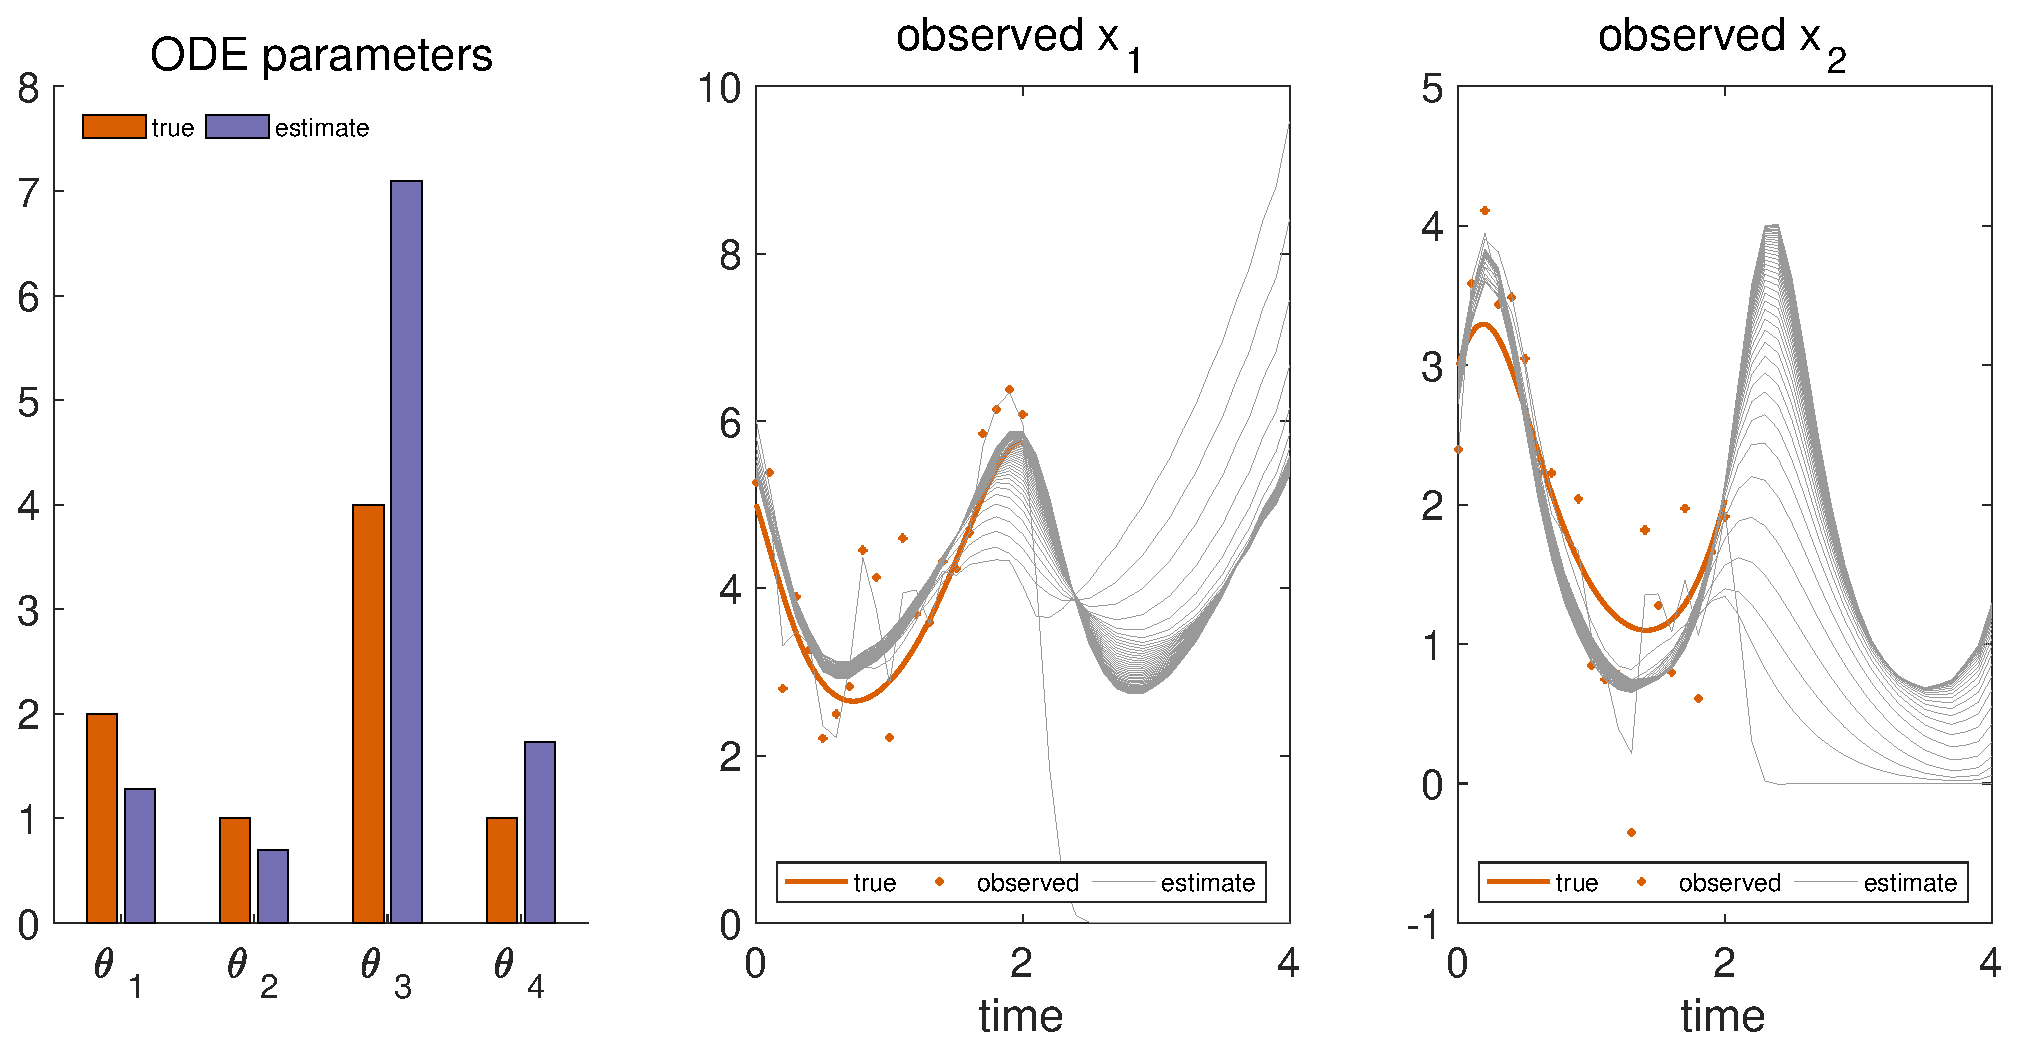
\includegraphics [width=5in]{VGM_for_Lotka_Volterra_41.eps}

}
\begin{par}

\end{par} \vspace{1em}
\subsection{Proxy for individual states}


Expanding the proxy distribution in equation (12) over the individual state $\mathbf{x}_u$:
\vspace{1em}
    
$\hat{q}(\mathbf{x}_u) \stackrel{(a)}{\propto} \exp \left(
~ E_{Q_{-u}}  \ln ( p(\mathbf{x}_u \mid \boldsymbol\theta, \mathbf{X}_{-u},\boldsymbol\phi,\gamma)
p(\mathbf{x}_u  \mid\mathbf{Y},\boldsymbol\phi,\boldsymbol\sigma) ) ~ \right)\\ \qquad
~ \stackrel{(b)}{=} \exp\big( ~ E_{Q_{-u}} \ln     \mathcal{N}\left(\mathbf{x}_u
; -\mathbf{B}_{u}^+ \mathbf{b}_u,     ~\mathbf{B}_u^{+} ~ (\mathbf{A} + \mathbf{I}\gamma)
~     \mathbf{B}_u^{+T} \right) + E_{Q_{-u}} \ln    \mathcal{N}\left(\mathbf{x}_u
; \boldsymbol\mu_u(\mathbf{Y}), \boldsymbol\Sigma_u    \right) \big)\\ \qquad ~= \exp\big(
~ E_{Q_{-u}} \ln                \mathcal{N}\left(\mathbf{x}_u ; -\mathbf{B}_{u}^+
\mathbf{b}_u,                ~\mathbf{B}_u^{+} ~ (\mathbf{A} + \mathbf{I}\gamma)
~                \mathbf{B}_u^{+T} \right) + E_{Q_{-u}} \ln                \mathcal{N}\left(\mathbf{x}_u
; \boldsymbol\mu_u(\mathbf{Y}), \boldsymbol{\sigma}_u                \right) \big)$.
    
In (a) we decompose the full conditional into an ODE-informed
distribution and a data-informed distribution and in (b) we substitute the ODE-informed
distribution $p(\mathbf{x}_u \mid \boldsymbol\theta, \mathbf{X}_{-u},\boldsymbol\phi,\gamma)$
with its density given by equation (8).
    \color{RoyalPurple}\begin{verbatim}
            [state.proxy.mean{:,symbols.state_string},state.proxy.inv_cov] = ...
            proxy_for_ind_states(state.lin_comb,...
            state.proxy.mean{:,symbols.state_string},...
            param_proxy_mean',dC_times_invC,coupling_idx.states,...
            symbols,mu,inv_sigma,simulation.observed_states,...
            A_plus_gamma_inv,opt_settings);
\end{verbatim}
\color{black}
\color{RoyalPurple}\begin{verbatim}
end
\end{verbatim}
\color{black}
\begin{par}

\end{par} \vspace{1em}
\begin{par}
Final results
\end{par} \vspace{1em}
\color{RoyalPurple}\begin{verbatim}
plot_results(fig_handle,state.proxy,simulation,param_proxy_mean,...
   plot_handle,symbols,plot_settings,'final');
\end{verbatim}
\color{black}

{
\centering
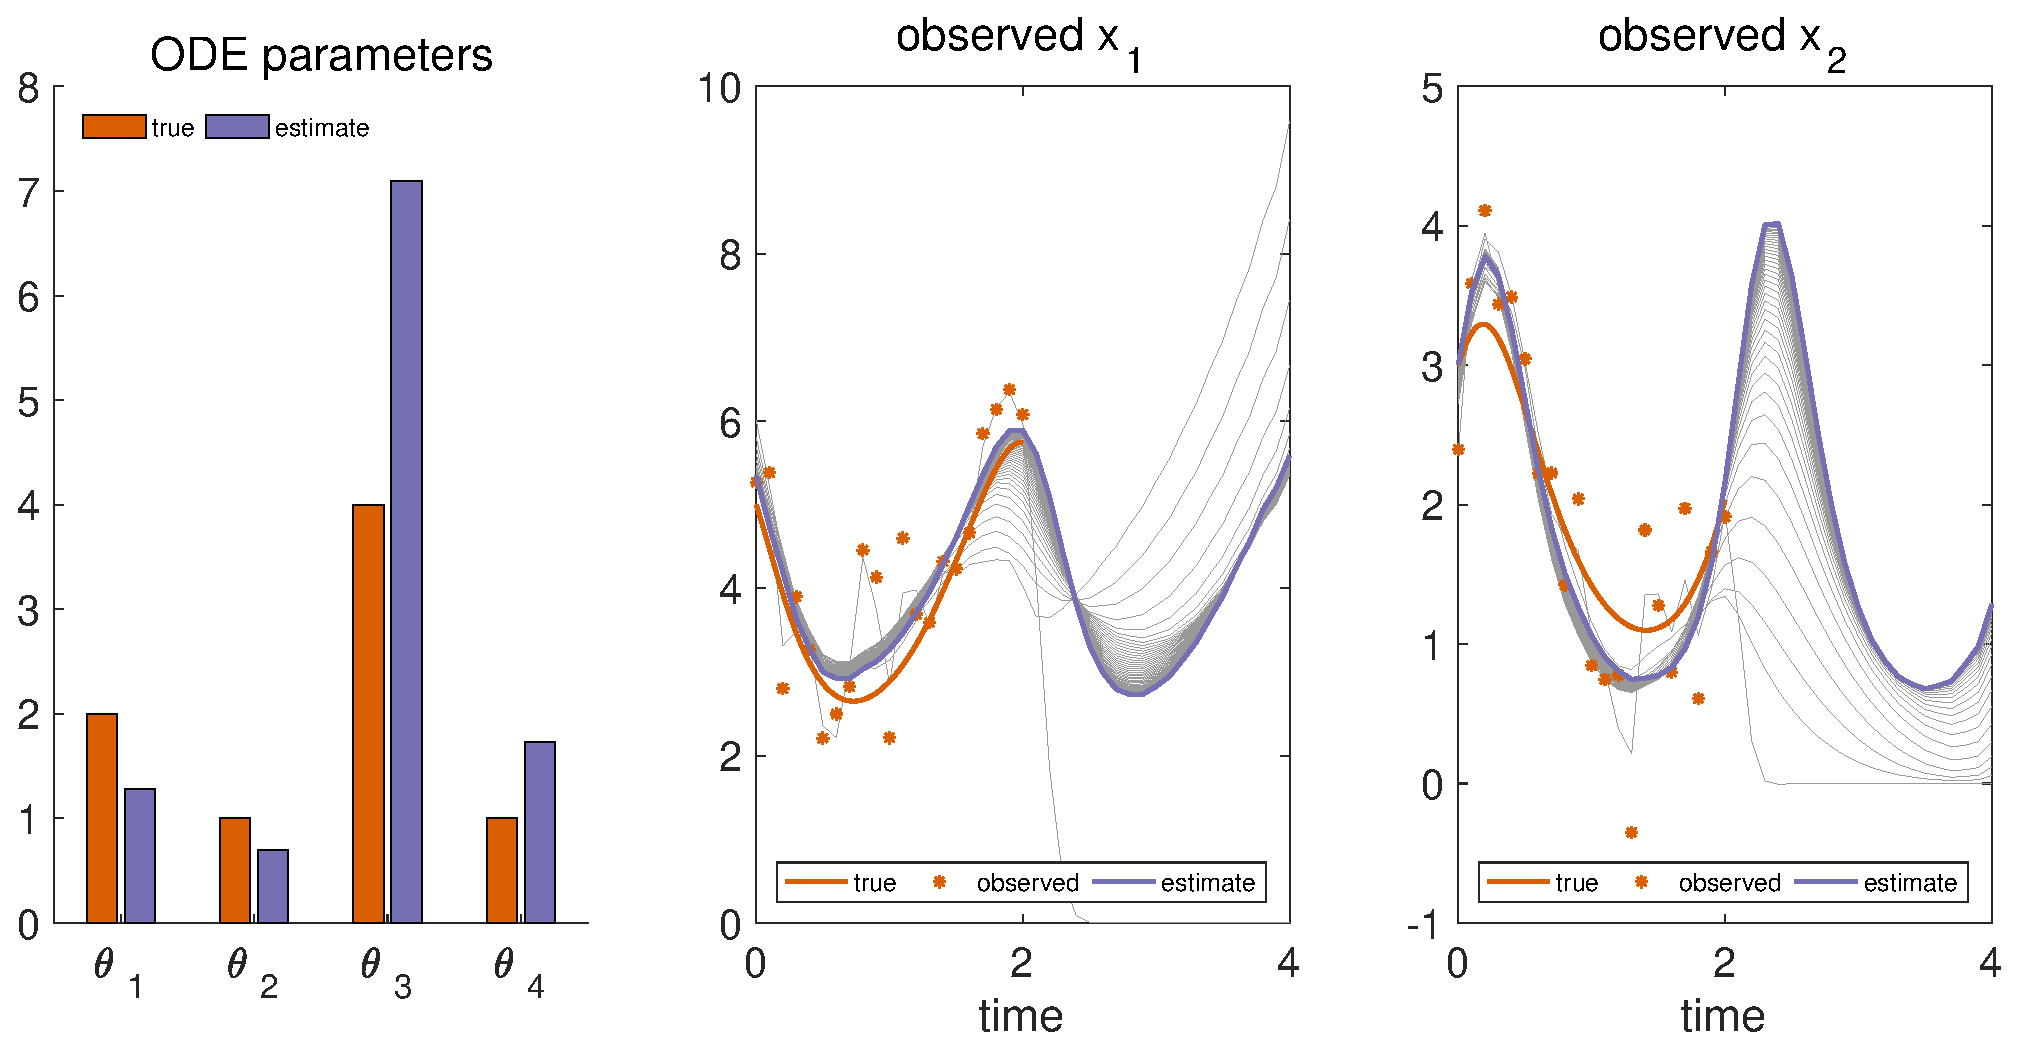
\includegraphics [width=5in]{VGM_for_Lotka_Volterra_42.eps}

}

\section{Time Taken}

\color{RoyalPurple}\begin{verbatim}
disp(['time taken: ' num2str(toc) ' seconds'])
\end{verbatim}
\color{black}
\color{black}

        \color{MidnightBlue}\begin{verbatim}time taken: 44.1589 seconds
\end{verbatim}
\color{black} 